%Template pembuatan naskah skripsi.
\documentclass{jtetiskripsi}

%Untuk prefiks pada daftar gambar dan tabel
\usepackage[titles]{tocloft}
\renewcommand\cftfigpresnum{Gambar\  }
\renewcommand\cfttabpresnum{Tabel\   }
\renewcommand{\arraystretch}{1.25}

%Untuk hyperlink dan table of content
\usepackage{hyperref}
\newlength{\mylenf}
\settowidth{\mylenf}{\cftfigpresnum}
\setlength{\cftfignumwidth}{\dimexpr\mylenf+2em}
\setlength{\cfttabnumwidth}{\dimexpr\mylenf+2em}
\usepackage{hyphenat}
\tolerance=1
\emergencystretch=\maxdimen
\hyphenpenalty=10000
\hbadness=10000

%Untuk Bold Face pada Keterangan Gambar
\usepackage[labelfont=bf]{caption}

%Untuk caption dan subcaption
\usepackage{caption}
\usepackage{subcaption}


%-----------------------------------------------------------------
%Disini awal masukan untuk data proposal skripsi
%-----------------------------------------------------------------
\titleind{Rancang Bangun Sistem Informasi Penggajian Karyawan Berbasis Web Menggunakan Framework Codeigniter
dengan Metode Extreme Programming
(Studi Kasus di Universitas Proklamasi 45 Yogyakarta)}

\fullname{Devara Eko Katon Mahardika}

\idnum{13650044}

\approvaldate{30 Januari 2018}

\degree{Sarjana Komputer}

\yearsubmit{2018}

\program{Teknik Informatika}

\dept{Teknik Informatika}

\firstsupervisor{Maria Ulfa Siregar, S.Kom. MIT.}
\firstnip{19780106 200212 2 001}

\secondsupervisor{Nama Dosen 2}
\secondnip{NIP Dosen 2}

%-----------------------------------------------------------------
%Disini akhir masukan untuk data proposal skripsi
%-----------------------------------------------------------------

\begin{document}

\cover

\clearpage
\phantomsection
\addcontentsline{toc}{chapter}{\approvalname}
\approvalpage

\acc

\authenticity

%-----------------------------------------------------------------
%Disini awal masukan untuk Prakata
%-----------------------------------------------------------------
\preface
Assalamu'alaikum Wr. Wb.

\vspace{0.5cm}

\emph{Alhamdulillahirabil'alamin}, puji syukur atas kehadirat Allah SWT karena hanya dengan rahmat dan hidayah-Nya, penulis dapat menyelesaikan penulisan skripsi ini yang berjudul "Rancang Bangun Sistem Informasi Penggajian Karyawan Berbasis Web Menggunakan \emph{Framework Codeigniter} dengan Metode \emph{Extreme Programming} (Studi Kasus di Universitas Proklamasi 45 Yogyakarta)" dengan lancar dan tanpa suatu halangan apapun. Tak lupa sholawat serta salam senantiasa terucarahkan kepada Baginda Rasul Muhammad SAW, semoga kita mendapatkan syafaatnya di Yaumul Qiyamah kelak.

Keberhasilan dalam penulisan skripsi ini yang mana menjadi salah satu syarat penyelesaian program sarjana Teknik Informatika Fakultas Sains dan Teknologi UIN Sunan Kalijaga, tidak lepas dari bantuan berbagai pihak yang dengan tulus dan ikhlas telah memberikan masukan kepada penulis. Oleh karena itu dalam kesempatan ini penulis mengucapkan terima kasih yang sebesar-besarnya kepada:

\begin{enumerate}
\itemsep0em
\item Bapak Prof. Dr. KH. Yudian Wahyudi, M.A., P.hD., selaku Rektor UIN Sunan Kalijaga Yogyakarta;
\item Bapak Dr. Murtono, M.Si., selaku Dekan Fakultas Sains dan Teknologi UIN Sunan Kalijaga Yogyakarta; 
\item Bapak Dr. Bambang Sugiantoro, M.T, selaku Ketua Program Studi Teknik Informatika Fakultas Sains dan Teknologi UIN Sunan Kalijaga Yogyakarta;
\item Ibu Dr. Shofwatul 'Uyun, S.T., M.Kom., selaku Dosen Pembimbing Akademik yang telah memberikan arahan serta masukan selama masa perkuliahan;
\item Ibu Maria Ulfa Siregar, S.Kom., MIT., selaku Dosen Pembimbing Skripsi yang telah membimbing serta memberikan koreksi selama pengerjaan skripsi ini;
\item Seluruh dosen dan staf Program Studi Teknik Informatika Fakultas Sains dan Teknologi UIN Sunan Kalijaga Yogyakarta;
\item Segenap staf Universitas Proklamasi 45 Yogyakarta yang telah membantu dalam menyelesaikan skripsi ini;
\item Kedua orang tua dan keluarga yang selalu memberikan cinta dan kasih sayang serta doa dan dukungannya;
\item Keluarga besar PMII Rayon Aufklarung, khususnya sahabat Korp Frekuensi yang selalu menemani saat suka maupun duka, serta memberikan semangat selama masa perkuliahan;
\item Teman-teman seperjuangan Program Studi Teknik Informatika Fakultas Sains dan Teknologi UIN Sunan Kalijaga Yogyakarta;
\item Semua pihak yang tidak dapat penulis sebutkan satu persatu yang telah membantu dalam proses penyelesaian skripsi ini.

\end{enumerate}

Penulis menyadari bahwa penulisan skripsi ini jauh dari kata sempurna dan masih banyak kekurangan. Kritik dan saran kepada penulis sangat diharapkan guna menyempurnakannya. Semoga skripsi ini dapat memberikan manfaat bagi pembaca maupun peneliti selanjutnya.

\vspace{0.5cm}

Wassalamu'alaikum Wr. Wb.

\begin{tabular}{p{7.5cm}c}
&Yogyakarta, 31 Agustus 2018\\
& Penulis \\
&\\
& \underline{Devara Eko K M} \\
& 13650044
\end{tabular}

%-----------------------------------------------------------------
%Disini awal masukan Acknowledment
%-----------------------------------------------------------------
\acknowledgment
Halaman ini penulis persembahkan kepada semua pihak yang telah membantu dan memberi dukungan kepada penulis, sebagai berikut:
\begin{enumerate}
    \itemsep0em
    \item Orang tua tercinta, khususnya Ibunda atau Mamak Sumilah yang telah membesarkan anak satu-satunya sehingga menjadi seperti sekarang ini dan tak lupa selalu memberikan doa serta nasehat kepada penulis.
    \item Dosen-dosen TIF, Pak Bambang, Pak Agus, Pak Sumarsono, Pak Aulia, Pak Nur, Pak Rahmat, Pak Didik, Pak Mustakim, Bu Uyun, Bu Ade, dan Bu Maria, terima kasih atas ilmu yang telah diberikan selama di bangku perkuliahan, semoga dapat bermanfaat dikemudian hari.
    \item \textbf{Pergerakan Mahasiswa Islam Indonesia} (PMII), tanpa ber-PMII saya tidak bisa menjadi seperti sekarang ini. Dan di sinilah saya membuktikan bahwa orang PMII juga cinta terhadap teknologi serta membuktikan kualitasnya.
    \item Sahabat/i tercinta, PMII KORP FREKUENSI 2013 yang telah melewati suka duka bersama dalam proses berorganisasi selama ini.
    \item Keluarga besar PMII RAYON AUFKLARUNG yang memberikan banyak pelajaran berharga dalam menapaki hiruk pikuknya perjalanan ini, serta menyadarkan saya bahwa kuliah di informatika tidak hanya sekedar ngoding, tetapi masih banyak hal berguna yang dapat dilakukan.
    \item TRI MURBA, Moh. Fahrizal Yusuf dan Dienda Lora Buana, semoga seluruh pengalaman perjuangan kita dapat terkenang selalu.
    \item Teman-teman TFORGAS satu angkatan, yang tidak dapat penulis sebutkan semuanya.
    \item Teman-teman pengurus HMPS Teknik Informatika periode 2015-2017, Aya, Anisa, Dini, Darma, Agil, dan semua yang tidak dapat disebutkan satu persatu.
    \item Adik-adik angkatanku tercinta, Nafi, Anisa, Ozi, Dani, Riko, Zidni, Irsa, Hasan, Fauzan, dkk, terimakasih telah menjadi tonggak estafet HMPS Teknik Informatika kedepan.
    \item Kepada orang-orang yang selalu memberikan semangat dan motivasi dalam menyelesaikan skripsi ini, Lisda Meilinda, Wayan Syafi'i, Dudi Arya Guntara, Markisinta, Dwi Kumala Mursyid, Mirza Firdaus Avecina, dan semua yang tidak bisa disebutkan satu persatu.
    \item Rekan-rekan kerja di Universitas Proklamasi 45 Yogyakarta yang selalu memberikan dukungan dalam penyelesaian skripsi ini.
    \item Seluruh pecinta teknologi, khususnya bahasa pemrograman, yang telah saling \emph{sharing online} dalam berbagi dan membantu dalam pemecahan suatu masalah.
\end{enumerate}


\motto
Seseorang tidak akan memperjuangkan perubahan dari ketidakbenaran menjadi kebenaran ketika yang harus ia perlihara adalah kemapanannya dalam ketidakbenaran. - Emha Ainun Nadjib

%-----------------------------------------------------------------
%Disini akhir masukan untuk muka skripsi
%-----------------------------------------------------------------
\begin{onehalfspace}
\clearpage
\phantomsection
\addcontentsline{toc}{chapter}{DAFTAR ISI}
\tableofcontents
\clearpage
\phantomsection
\addcontentsline{toc}{chapter}{DAFTAR TABEL}
\listoftables
\clearpage
\phantomsection
\addcontentsline{toc}{chapter}{DAFTAR GAMBAR}
\listoffigures
\end{onehalfspace}

%-----------------------------------------------------------------
%Disini awal masukan Intisari
%-----------------------------------------------------------------
\begin{abstractind}
\begin{center}
    \textbf{RANCANG BANGUN SISTEM INFORMASI PENGGAJIAN KARYAWAN BERBASIS WEB MENGGUNAKAN \emph{FRAMEWORK CODEIGNITER} DENGAN METODE \emph{EXTREME PROGRAMMING}}\\
    \textbf{(STUDI KASUS DI UNIVERSITAS PROKLAMASI 45 YOGYAKARTA)}
\end{center}

\begin{center}
    \textbf{\underline{Devara Eko Katon Mahardika}\\NIM.13650044}
\end{center}

\begin{center}
    \textbf{INTISARI}
\end{center}

Universitas Proklamasi 45 Yogyakarta adalah universitas swasta yang dibawahi oleh suatu Yayasan yang telah menerapkan berbagai sistem informasi di berbagai bidang kerjanya. Akan tetapi dalam proses penggajian karyawannya masih dilakukan secara manual dan belum memanfaatkan sistem yang terkomputerisasi, seperti rekap absensi, rekap upah selain gaji pokok, serta penjumlahan gaji yang diterima oleh karyawan. Hal tersebut membuat proses penggajian menjadi kurang efektif dan efisien. Penelitian ini bertujuan untuk membangun sistem usulan yaitu sistem informasi penggajian karyawan berbasis web pada Universitas Proklamasi 45 Yogyakarta dengan bahasa pemrograman PHP menggunakan Fremework Codeigniter dan MySQL sebagai basis datanya.

Metode pengembangan sistem yang digunakan adalah metode \emph{Extreme Programming}. Metode ini dipilih karena sangat mengedepankan komunikasi yang intens antara klien dengan pengembang sistem sehingga ketika terdapat perubahan ataupun kesalahan dalam sistem, pengembang selalu siap untuk memperbaikinya. \emph{Extreme Programming} juga memiliki tahapan yang sederhana, yaitu \emph{planning}, \emph{design}, \emph{coding}, dan \emph{testing}

Hasil dari penelitian ini adalah dihasilkannya sistem informasi penggajian karyawan berbasis web yang memiliki berbagai aktor yang terlibat dalam pengelolaan dan pengolahan datanya. Dengan adanya sistem informasi ini, proses penggajian karyawan menjadi lebih efektif dan efisien, karena data penggajian diproses dan dihitung oleh sistem sehingga memiliki tingkat akurasi data yang tinggi serta tidak membutuhkan waktu yang lama dalam proses perhitungannya.

\bigskip
\noindent
\textbf{Kata kunci :} Berbasis Web, Sistem Informasi, Sistem Informasi Penggajian, \emph{Codeigniter}, \emph{Extreme Programming}.
\end{abstractind}

\begin{abstracteng}
\begin{center}
    \textbf{DESIGN AND DEVELOPMENT OF WEB BASED EMPLOYEE PAYROLL INFORMATION SYSTEM USING CODEIGNITER FRAMEWORK AND EXTREME PROGRAMMING METHOD}\\
    \textbf{(CASE STUDY AT UNIVERSITY OF PROCLAMATION 45 YOGYAKARTA)}
\end{center}

\begin{center}
    \textbf{\underline{Devara Eko Katon Mahardika}\\NIM.13650044}
\end{center}

\begin{center}
    \textbf{ABSTRACT}
\end{center}

Universitas Proklamasi 45 Yogyakarta is a private university which is supervised by a Foundation that has implemented various information systems in various fields of work. However, in the payroll process the employees are still done manually and have not utilized a computerized system, such as attendance recap, wage recapitulation in addition to basic salary, as well as the sum of salary received by employees. This makes the payroll process less effective and efficient. This study aims to establish a proposed system that is a web-based employee payroll information system at the Universitas Proklamasi 45 Yogyakarta with the PHP programming language using Fremework Codeigniter and MySQL as its database.

The system development method used is the Extreme Programming method. This method was chosen because it promotes intense communication between the client and the system developer so that when there are changes or errors in the system, the developer is always ready to fix it. Extreme Programming also has a simple stage, namely planning, design, coding, and testing.

The results of this study are the result of a web-based employee payroll information system that has various actors involved in the management and processing of its data. With this information system, the employee payroll process becomes more effective and efficient, because payroll data is processed and calculated by the system so that it has a high level of data accuracy and does not require a long time in the calculation process.

\bigskip
\noindent
\textbf{\emph{Keywords :}} \emph{Web Application, Information System, Payroll System, Codeigniter, Extreme Programming}.
\end{abstracteng}
%-----------------------------------------------------------------
%Disini akhir masukan Intisari
%-----------------------------------------------------------------

%-----------------------------------------------------------------
%Disini awal masukan untuk Bab
%-----------------------------------------------------------------
%!TEX root = ./template-skripsi.tex
%-------------------------------------------------------------------------------
% 								BAB I
% 							LATAR BELAKANG
%-------------------------------------------------------------------------------

\chapter{PENDAHULUAN}

\section{Latar Belakang}
Kemajuan teknologi dewasa ini mengalami perkembangan yang sangat pesat dalam berbagai bidang. Hal tersebut ditandai dengan penerapan sistem pelayanan yang sudah terkomputerisasi di berbagai instansi, baik itu perusahaan, rumah sakit, sekolah, maupun universitas. Penerapan sistem yang terkomputerisasi pada berbagai sektor memberikan kemudahan baik bagi perusahaan yang bersangkutan maupun bagi pengguna informasi dalam rangka mencari suatu informasi dengan cepat dan tepat. Banyak perusahaan berlomba-lomba mengimplementasikan sistem yang serba terkomputerisasi yang sesuai dengan kebutuhan perusahaan tersebut dengan tujuan meningkatkan dan mengoptimalkan kualitas layanan mereka. Bahkan tidak sedikit perusahaan yang mencantumkan penerapan suatu sistem yang terkomputerisasi dalam visi misi mereka.

Salah satu sistem yang banyak digunakan di sebuah perusahaan dalam rangka mengoptimalkan kualitas layanan meraka adalah penerapan suatu sistem informasi penggajian, yang diharapkan dapat membantu dan mempermudah dalam melakukan proses penggajian karyawan. Penerapan sistem informasi penggajian tersebut sangat berpengaruh pada perusahaan atau instansi yang memiliki jumlah tenaga kerja yang cukup banyak. Lebih lanjut lagi, komponen upah atau gaji karyawan tidak hanya gaji pokok saja, tetapi juga termasuk berbagai tunjangan, insentif, potongan, lembur dan upah lain di luar gaji pokok. Besaran gaji masing-masing tenaga kerja juga berbeda. Apabila proses perhitungan gaji masih manual, dapat merugikan perusahaan dalam hal efisiensi waktu, yaitu akan memakan waktu yang cukup lama, sehingga dapat mengakibatkan keterlambatan dalam pembayaran atau pemberian gaji kepada karyawan.

Universitas Proklamasi 45 Yogyakarta adalah universitas swasta yang pengelolaannya dibawahi oleh suatu Yayasan. Dalam setiap bidang kerjanya hampir semua telah memanfaatkan sistem informasi guna mempermudah pekerjaan dan tata kelola manajerialnya. Namun dalam proses penggajian karyawan, belum efektif dan efisien karena prosesnya bersifat manual atau tidak memanfaatkan suatu sistem informasi, sehingga masih memiliki beberapa kekurangan. Kekurangan tersebut diantaranya adalah proses penggajian yang memakan waktu cukup lama, akurasi perhitungan data dan dokumentasi data tidak tertata dengan baik. Salah satu yang membuat proses penggajian memakan waktu yang cukup lama adalah kegiatan rekap data yang mempengaruhi besaran nominal gaji dihitung secara manual, seperti rekap absensi karyawan, rekap data lembur, dan rekap upah lain selain gaji pokok.  Oleh karena itu, diperlukan adanya sebuah sistem informasi penggajian karyawan yang tepat guna, efisien dan efektif untuk digunakan dalam proses perhitungan gaji karyawan di Universitas Proklamasi 45 Yogyakarta.

Dalam melakukan perancangan sistem informasi, terdapat permasalahan yang sering terjadi, yaitu permintaan perubahan \emph{requirement} dan penambahan fitur pada sistem yang diinginkan oleh klien ketika proses perancangan sistem dilakukan. Maka dari itu, diperlukan metode pengembangan sistem yang sederhana dan melibatkan klien dalam hal berkomunikasi dengan pengembang sistem. Metode \emph{Extreme Programming} merupakan salah satu metodologi \emph{Agile} yang menekankan komunikasi yang baik dengan klien, cepat dalam proses pengembangan, serta siap dalam menerima perubahan dan perbaikan setiap kali terdapat kesalahan. Oleh karena itu, metode \emph{Extreme Programming} digunakan dalam perancangan sistem informasi penggajian karyawan ini.

\section{Rumusan Masalah}
Berdasarkan latar belakang di atas, dapat dirumuskan suatu masalah sebagai berikut:
\begin{enumerate}
\itemsep0em
\item Bagaimana menganalisis dan merancang sistem informasi penggajian karyawan berbasis web di Universitas Proklamasi 45 Yogyakarta?
\item Bagaimana mengimplementasikan sistem informasi tersebut ke dalam proses penggajian karyawan di Universitas Proklamasi 45 Yogyakarta sehingga nantinya dapat menjadi sistem informasi yang tepat guna?
\item Bagaimana menganalisis efektifitas dan efisiensi dari penggunaan sistem informasi penggajian karyawan di Universitas Proklamasi 45 Yogyakarta dari segi hasil dan waktu?
\end{enumerate}

\section{Batasan Masalah}
Adapun pembatasan masalah dalam suatu penelitian sangat diperlukan agar penelitian lebih terarah dan memudahkan dalam pembahasan, sehingga tujuan penelitian dapat tercapai. Batasan masalah dalam merancang sistem informasi ini adalah sebagai berikut:
\begin{enumerate}
\itemsep0em
\item Proses perhitungan gaji pada Sistem Informasi Penggajian Karyawan ini disesuaikan dengan kebutuhan \emph{project owner};
\item Sistem Informasi Penggajian Karyawan ini memiliki beberapa kategori pengguna sesuai wewenang jabatannya dan disesuaikan dengan kebutuhan \emph{project owner}.
\end{enumerate}

\section{Tujuan Penelitian}
Berdasarkan rumusan masalah di atas, maka tujuan yang ingin diperoleh dari penelitian ini adalah:
\begin{enumerate}
\itemsep0em
\item Menganalisis dan merancang Sistem Informasi Penggajian Karyawan berbasis web di Universitas Proklamasi 45 Yogyakarta;
\item Mengimplementasikan sistem informasi tersebut ke dalam proses penggajian karyawan di Universitas Proklamasi 45 Yogyakarta sehingga menjadi sistem informasi yang tepat guna;
\item Menganalisis efektifitas dan efisiensi dari penggunaan sistem informasi penggajian karyawan di Universitas Proklamasi 45 Yogyakarta dari segi hasil dan waktu.
\end{enumerate}

\section{Manfaat Penelitian}
    Manfaat penelitian yang diharapkan yaitu:
    \begin{enumerate}
        \itemsep0em
        \item Menambah ilmu pengetahuan dan pengalaman penulis dalam mengembangkan suatu sistem informasi dari mulai tahap analisis, perancangan, implementasi dan pengujian sehingga menjadi sistem informasi yang tepat guna.
        \item Membantu dan mempermudah pihak perusahaan dalam melakukan suatu pekerjaan, contohnya proses penggajian. Kedepannya juga memungkinkan adanya pengembangan sistem lebih lanjut apabila diperlukan sesuai dengan kebutuhan.
        \item Dapat dijadikan sebagai referensi penelitian di waktu yang akan datang.
    \end{enumerate}

\section{Sistematika Penulisan}
\begin{enumerate}
    \itemsep0em
    \item \textbf{BAB I : PENDAHULUAN}
    
    Pada bab ini dijelaskan latar belakang, rumusan masalah, batasan, tujuan, manfaat, dan sistematika penulisan.
    \item \textbf{BAB II : TINJAUAN PUSTAKAN DAN LANDASAN TEORI}
    
    Pada bab ini dijelaskan teori-teori dan penelitian-penelitian sejenis sebelumnya yang digunakan sebagai acuan atau referensi dan dasar dalam melakukan penelitian.
    \item \textbf{BAB III : METODE PENGEMBANGAN SISTEM}
    
    Pada bab ini dijelaskan metode pengembangan sistem yang digunakan selama penelitian ini yang meliputi alur atau tahapan dalam melakukan perancangan sistem.
    \item \textbf{BAB IV : ANALISIS DAN PERANCANGAN}
    
    Pada bab ini dijelaskan bagaimana mengalisis objek penelitian dan permasalahan dalam penelitian serta langkah-langkah perancangan dalam menyelesaikan solusi permasalahan.
    \item \textbf{BAB V : IMPLEMENTASI DAN PENGUJIAN}
    
    Pada bab ini dijelaskan bagaimana mengimplementasikan hasil perancangan solusi permasalahan ke dalam suatu wadah yang dapat digunakan, serta menjelaskan tahapan-tahapan pengujian.
    \item \textbf{BAB VI : HASIL DAN PEMBAHASAN}
    
    Pada bab ini dijelaskan hasil dan pembahasan dari pengimplementasian penelitian dan juga hasil pengujian sistem.
    \item \textbf{BAB VII : PENUTUP}
    
    Pada bab ini dijelaskan kesimpulan dari hasil penelitian serta saran-saran yang dapat digunakan di masa yang akan mendatang ketika akan melakukan penelitian sejenis.
\end{enumerate}

% Baris ini digunakan untuk membantu dalam melakukan sitasi
% Karena diapit dengan comment, maka baris ini akan diabaikan
% oleh compiler LaTeX.
\begin{comment}
\bibliography{daftar-pustaka}
\end{comment}


%!TEX root = ./template-skripsi.tex
%-------------------------------------------------------------------------------
%                            BAB II
%               TINJAUAN PUSTAKA DAN DASAR TEORI
%-------------------------------------------------------------------------------

\chapter{TINJAUAN PUSTAKA DAN LANDASAN TEORI}                

\section{Tinjauan Pustaka}
  Penelitian yang dilakukan oleh Alhadi (2013) yang bertujuan merancang sistem informasi penggajian dan pengupahan dengan analisis data dan proses bisnis yang ada pada Bagian Sumber Daya dan Umum PT. Krakatau Wajatama Cilegon, Banten. Hasil yang diperoleh adalah sistem menjadi mudah untuk dipelihara dan dikembangkan, dan mampu mengurangi resiko terjadinya masalah dalam hal pengembangan dan perbaikan sistem yang disebabkan oleh pergantian pengembang sistem.

  Penelitian yang dilakukan oleh Dewanto (2013) yang dilakukan di penerbit buku pendidikan Deepublish Yogyakarta. Penelitian tersebut menghasilkan paket sistem informasi untuk menghitung \emph{cost of production} (biaya produksi) dan penggajian karyawan serta memudahkan dalam perhitungannya serta evaluasi keungan secara berkala.

  Penelitian yang dilakukan oleh Firdaus (2017) yang bertujuan merancang aplikasi sistem informasi penggajian di CV. Sogan Jaya Abadi. \emph{Output} yang dihasilkan adalah proses penggajian karyawan lebih cepat dan akurat serta pengaksesan informasi bisa dilakukan dimanapun dan kapanpun.
  
  Penelitian yang dilakukan oleh Hutama (2016) yang bertujuan untuk merancang perangkat lunak berbasis Android untuk digitalisasi presensi karyawan di PT. Geschool Cerdas Mandiri. Hasil dari penelitian ini adalah perangkat lunak yang dirancang dapat digunakan untuk melakukan manajemen data jam kerja karyawan.
  
  Berdasarkan hasil dari penelitian yang telah disebutkan diatas, \emph{output} yang dihasilkan dan metode yang digunakan dalam pengembangan berbeda-beda. Perbedaan penelitian ini dengan penelitian sebelumnya adalah sistem yang dikembangkan ini memiliki fungsionalitas yang cukup lengkap dengan berbagai aktor yang terlibat dalam pengolahan datanya sesuai dengan hak akses atau wewenang masing-masing aktor. Detail perbandingan penelitian terdahulu yang dijadikan sebagai tinjauan pustaka dapat dilihat pada Tabel.
  \begin{spacing}{1.25}
  \begin{longtable}{|>{\centering}p{1.5em}|p{2cm}|>{\raggedright}p{3cm}|p{3cm}|>{\raggedright}p{4cm}|}
  \caption{Perbedaan Penelitian.}
  \label{perbandingan} \\
  \hline \textbf{No.} & \textbf{Peneliti} & \textbf{Domain} & \textbf{Metode Pengembangan} & \textbf{Hasil}  \\ \hline
  \endfirsthead
  \multicolumn{5}{c}%
  {{\bfseries \tablename\ \thetable{}:} Perbandingan Penelitian (lanjutan)} \\
  \hline \textbf{No.} & \textbf{Peneliti} & \textbf{Domain} & \textbf{Metode Pengembangan} & \textbf{Hasil}  \\ \hline
  \endhead
  \hline
  \endfoot
  \hline \hline
  \endlastfoot
  1. & Alhadi (2013) & Penggajian dan pengupahan karyawan & SDLC & Sistem penggajian dan pengupahan yang termodulisasi, memiliki standar aturan dalam proses pengembangan program \\ \hline
  2. & Dewanto (2013) & \emph{Cost of Production} (COP) dan penggajian karyawan & \emph{Prototyping} & Sistem informasi yang dapat membantu dalam menghitung total gaji berdasar kriteria yang terkait dan perhitungan biaya produksi yang mencakup pengolahan waktu produksi, biaya proses produksi \\ \hline
  3. & Firdaus (2017) & Penggajian karyawan & \emph{Prototyping} & Hak akses pengguna sistem ada empat, yaitu \emph{superadmin}, \emph{hrd}, \emph{finance}, dan direktur perusahaan dengan tujuan utama untuk memaksimalkan proses manajemen karyawan dan penggajian karyawan \\ \hline
  4. & Hutama (2016) & Presensi karyawan & \emph{Extreme Programming} & Aplikasi presensi berbasis android yang memiliki fitur sebagai alat presensi, mengirim permintaan izin, dan melihat laporan presensi \\ \hline
  5. & Usulan (2018) & Penggajian Karyawan & \emph{Extreme Programming} & Sistem informasi penggajian karyawan berbasis web yang dalam pengembangannya melalui beberapa siklus dan dapat menyesuaikan kebutuhan \emph{project owner} agar dihasilkan sistem yang tepat guna dan dapat mambantu dan memudahkan proses penggajian karyawan  \\ \hline
  \end{longtable}
  \end{spacing}
  \vspace{4mm}
  
\section{Landasan Teori}

\subsection{Sistem Informasi}

    \subsubsection{Pengertian Sistem}
    Sistem didefinisikan ke dalam dua kelompok pendekatan, yaitu pendekatan yang menekankan pada prosedurnya dan pendekatan yang menekankan pada komponen dan elemennya. Menurut Jerry FitzGeral dalam bukunya yang berjudul \emph{Fundamentals of Systems Analysis} (1981) mendefinisikan pendekatan sistem yang lebih menekankan pada prosedurnya adalah suatu jaringan kerja dari prosedur-prosedur yang saling berhubungan, berkumpul bersama-sama untuk melakukan suatu kegiatan atau untuk menyelesaikan suatu sasaran yang tertentu. Sedangkan pendekatan yang menekankan pada komponen atau elemennya menyebutkan bahwa sistem adalah kumpulan komponen yang saling berkaitan dan bekerjasama untuk mencapai suatu tujuan tertentu (Ladjamudin, 2005).
    
    \subsubsection{Karakteristik Sistem}
    Untuk membedakan suatu sistem dengan sistem yang lainnya, maka diperlukan sekumpulan karakteristik pada sistem tersebut (Ladjamudin, 2005). Berikut merupakan beberapa karakteristik sistem:
    \begin{enumerate}
        \itemsep0em
        \item Batasan Sistem (\emph{Boundary})
        
        Daerah yang membataskan satu sistem dengan sistem yang lain maupun dengan lingkungan luar dan menunjukan ruang lingkup dari sistem tersebut.
        \item Lingkungan Luar Sistem (\emph{Environment})
        
        Segala sesuatu yang berada di luar sistem yang mempengaruhi operasi sistem. Lingkungan luar sistem dapat bersifat positif (menguntungkan) maupun negatif (merugikan).
        \item Masukan Sistem (\emph{Input})
        
        Energi yang dimasukan ke dalam sistem, dapat berupa perawatan (\emph{maintenance input}) dan masukan sinyal (\emph{signal input}). \emph{Maintenance input} adalah energi yang dimasukan agar sistem tersebut dapat berjalan. \emph{Signal input} adalah enegi yang diproses untuk menghasilkan keluaran (\emph{output}).
        \item Keluaran Sistem (\emph{Output})
        
        Keluaran adalah hasil dari energi yang telah diolah, dapat diklasifikasikan menjadi keluaran yang berguna dan sisa pembuangan. Keluaran dapat merupakan masukan untuk subsistem lain.
        \item Komponen Sistem (\emph{Component})
        
        Suatu sistem terdiri dari beberapa komponen yang saling berinteraksi, saling kerjasama membentuk suatu kesatuan. Komponen atau elemen-elemen dalam sistem ini dapat berupa subsistem ataupun bagian-bagian dari sistem.
        \item Penghubung Sistem (\emph{Interface})
        
        Penghubung merupakan media yang menghubungkan antara satu subsistem dengan subsitem lainnya, melalui penghubung ini memungkinkan sumber-sumber daya mengalir dari satu subsistem ke subsistem lainnya.
        \item Proses Sistem (\emph{Process})
        
        Proses sistem merupakan tempat pengolahan masukan (\emph{Input}) menjadi keluaran (\emph{Output}).
        \item Sasaran dan Tujuan Sistem
        
        Suatu sistem memiliki suatu tujuan atau sasaran. Tanpa adanya tujuan atau sasaran maka operasi sistem tidak akan berarti.
    \end{enumerate}
    
    \subsubsection{Pengertian Data dan Informasi}
    Dalam Ladjamudin (2005), data merupakan kenyataan yang menggambarkan suatu kejadian-kejadian dan kesatuan nyata. Sedangkan menurut Haryanto (2004), data adalah rekaman mengenai fenomena / fakta yang ada atau sedang terjadi. Dari dua definisi tersebut penulis dapat menyimpulkan bahwa data merupakan fakta dari sesuatu atau kejadian yang kita hadapi.

    Menurut Jogiyanto (2005) informasi adalah data yang diolah menjadi bentuk yang lebih berguna dan lebih berarti bagi yang menerimanya. Adapun Davis dalam (Ladjamudin, 2005) mendefinisikan informasi sebagai data yang telah diolah menjadi bentuk yang lebih berarti dan berguna bagi penerimanya untuk mengambil keputusan masa kini maupun yang akan datang. Dari dua definisi di atas penulis dapat menyimpulkan bahwa pengertian informasi adalah data yang telah diolah menjadi bentuk yang lebih berguna dan dapat memberikan nilai bagi penerimanya.

    \subsubsection{Pengertian Sistem Informasi}
    Menurut Leitch dan Davis, sistem informasi adalah suatu sistem di dalam suatu orgasisasi yang mempertemukan kebutuhan pengolahan transaksi, mendukung operasi, bersifat \emph{managerial} dan kegiatan strategi dari suatu organisasi dan menyediakan pihak luar tertentu dengan laporan-laporan yang diperlukan (Jogiyanto, 2005). Sedangkan dalam Whitten (2006), sistem Informasi adalah sekelompok elemen-elemen dalam suatu organisasi yang saling berintegrasi dengan menggunakan masukkan, proses dan keluaran dengan maksud yang sama untuk mencapai suatu tujuan dan dapat digunakan untuk membantu pengambilan keputusan yang tepat.
    
    Dari dua definisi di atas, penulis menyimpulkan bahwa sistem informasi adalah suatu sistem yang menyediakan informasi untuk manajemen dalam mengambil keputusan dan juga untuk menjalankan operasional perusahaan, di mana sistem tersebut merupakan kombinasi dari orang-orang, teknologi informasi dan prosedur-prosedur yang tergorganisasi.
    
    \subsubsection{Komponen Sistem Informasi}
    Sistem informasi memiliki beberapa komponen tertentu (Ladjamudin, 2005), yang diklasifikasikan sebagai berikut:
        \begin{enumerate}
            \itemsep0em
            \item \emph{Hardware} dan \emph{software} berperan sebagai mesin;
            \item \emph{People} (manusia) merupakan pengguna mesin;
            \item \emph{Procedures} yaitu tatacara penggunaan mesin;
            \item Data yang merupakan penghubung antara manusia dan mesin agar terjadi proses pengolahan data.
        \end{enumerate}

\subsection{Konsep Basis Data}

    \subsubsection{Basis Data (\emph{Database})}
    Basis data adalah suatu pengorganisasian sekumpulan data yang saling terkait sehingga memudahkan aktivitas untuk memperoleh informasi. Basis data dimaksudkan untuk mengatasi masalah pada sistem yang memakai pendekatan berbasis berkas (Kadir, 2003).

    Tujuan awal dan utama dalam pengolahan data pada sebuah basis data adalah agar dapat mencari data dengan mudah dan cepat. Di samping itu, pemanfaatan data untuk pengolahan data juga memiliki tujuan-tujuan tertentu. Pemanfaatan basis data dilakukan untuk memenuhi sejumlah tujuan sebagai berikut (Kadir, 2003):
    \begin{enumerate}
      \itemsep0em
      \item Kecepatan dan kemudahan (\emph{Speed})

      Pemanfaatan basis data memungkinkan untuk dapat menyimpan data atau melakukan perubahan/ manipulasi terhadap data atau menampilkan kembali data tersebut dengan cepat dan mudah.
      \item Efisiensi ruang penyimpanan (\emph{Space})

      Penggunaan ruang penyimpanan di dalam basis data dilakukan untuk mengurangi jumlah \emph{redudansi} (pengulangan) data, baik dengan melakukan penerapan sejumlah pengkodean atau dengan membuat relasi-relasi (dalam bentuk \emph{file}) antar kelompok data yang saling berhubungan.
      \item Keakuratan (\emph{Accuracy})

      Pemanfaatan pengkodean atau pembentukan relasi antar data bersama dengan penerapan aturan/ batasan tipe data, domain data, keunikan data dan sebagainya dan diterapkan dalam basis data, sangat berguna untuk menentukan keakuratan pemasukan atau penyimpanan data.
      \item Ketersediaan (\emph{Availability})

      Pertumbuhan data (baik dari jumlah maupun jenisnya) sejalan dengan waktu akan semakin membutuhkan ruang penyimpanan yang besar. Data yang sudah jarang atau bahkan tidak pernah lagi digunakan dapat diatur untuk dilepaskan dari sistem basis data dengan cara penghapusan atau dengan memindahkannya ke media penyimpanan.
      \item Kelengkapan (\emph{Completeness})

      Lengkap atau tidaknya data yang dikelola bersifat relatif baik terhadap kebutuhan pemakai maupun terhadap waktu. Dalam sebuah basis data, struktur dari basis data tersebut juga harus disimpan. Untuk mengakomodasi kebutuhan kelengkapan data yang semakin berkembang, maka tidak hanya menambah \emph{record-record} data, tetapi juga melakukan penambahan struktur dalam basis data.
      \item Keamanan (\emph{Security})

      Sistem keamanan digunakan untuk dapat menentukan siapa saja yang boleh menggunakan basis data dan menentukan jenis operasi apa saja yang boleh dilakukan.
      \item Kebersamaan pemakai

      Pemakai basis data sering kali tidak terbatas hanya pada satu pemakaian saja atau oleh satu sistem aplikasi saja. Basis data yang dikelola oleh sistem (aplikasi) yang mendukung lingkungan \emph{multiuser}, akan dapat memenuhi kebutuhan ini, tetapi dengan menjaga/menghindari terhadap munculnya persoalan baru seperti inkonsistensi data (karena data yang sama diubah oleh banyak pemakai pada saat bersamaan).
    \end{enumerate}

    \subsubsection{DBMS (\emph{Database Management System})}
    DBMS (\emph{Database Management System}) merupakan koleksi terpadu dari \emph{database} dan program-program komputer yang digunakan untuk mengakses dan memelihara \emph{database}. Program-program tersebut menyediakan berbagai fasilitas operasi untuk memasukkan, melacak, dan memodifikasi data kedalam \emph{database}, mendefinisikan data baru, serta mengolah data menjadi informasi yang dibutuhkan (Ladjamudin, 2005).

    Tujuan utama DBMS adalah menyediakan lingkungan yang nyaman dan efisien untuk penyimpanan dan pengambilan data dari basis data. DBMS berperan memberi abstraksi data tingkat tinggi ke pemakai. Sedangkan tujuan lain dari DBMS antara lain (Hariyanto, 2004):
    \begin{enumerate}
      \itemsep0em
      \item Menghindari redudansi dan inkonsistensi data;
      \item Menghindari kesulitan pengaksesan data;
      \item Menghindari isolasi data;
      \item Menghindari terjadinya anomali pengaksesan konkuren;
      \item Menghindari masalah-masalah keamanan;
      \item Menghindari masalah-masalah integritas.
    \end{enumerate}
    
\subsection{Analisa dan Perancangan Sistem}
    Menurut Whitten (2004), analisa sistem adalah teknik pemecahan masalah dengan cara memecahkan sistem ke dalam komponen-komponen dengan tujuan mempelajari komponen tersebut bekerja dan berinteraksi untuk menyelesaikan tujuan mereka. Perancangan sistem merupakan pelengkap dari analisa sistem ke dalam suatu sistem yang utuh dengan tujuan mendapatkan sistem yang lebih baik.

    Ada enam tahap analisis sistem menurut Whitten (2004), yaitu:
    \begin{enumerate}
      \itemsep0em
      \item Menggunakan penelitian sistem;
      \item Mengorganisasikan tim proyek;
      \item Mendefinisikan kebutuhan informasi;
      \item Mendefinisikan kriteria kinerja sistem;
      \item Menyiapkan usulan rancangan;
      \item Menyetujui atau menolak rancangan proyek.
    \end{enumerate}

    Perancangan sistem adalah penentuan proses dan data yang diperlukan oleh sistem baru, jika sistem itu berbasis komputer, perancangan dapat menyertakan spesifikasi peralatan yang akan digunakan (McLeod, 2001).

    Adapun tahapan perancangan sistem sebagai berikut:
    \begin{enumerate}
      \itemsep0em
      \item Menyiapkan rancangan sistem yang terperinci;
      \item Mengidentifikasi berbagai alternatif sistem;
      \item Mengevaluasi berbagai alternatif konfigurasi sistem;
      \item Memilih konfigurasi terbaik;
      \item Menyiapkan usulan penerapan;
      \item Menyetujui atau menolak penerapan sistem.
    \end{enumerate}

    Dari berbagai penjelasan di atas, penulis dapat menyimpulkan bahwa analisa dan perancangan sistem adalah proses dimana menerjemahkan kebutuhan pemakai informasi ke dalam sebuah rancangan guna memenuhi kebutuhan dari pemakai informasi dan memberikan gambaran yang lebih jelas untuk dijadikan pertimbangan.
    
  \subsection{Gaji}
    \subsubsection{Pengertian Gaji}
    Gaji adalah balas jasa dalam bentuk uang yang diterima karyawan sebagai konsekuensi dan statusnya sebagai seorang karyawan yang memberikan kontribusi dalam mencapai tujuan perusahaan. Sedangkan menurut Rivai dan Sagala (2009), gaji dapat juga diartikan sebagai bayaran tetap yang diterima seseorang karena kedudukannya dalam perusahaan.
    
    \subsubsection{Tujuan Pemberian Upah dan Gaji}
    Berikut adalah tujuan dalam pemberian upah dan gaji (Rivai dan Sagala, 2009):
    \begin{enumerate}
        \itemsep0em
        \item Ikatan Kerja Sama
        
        Dengan pemberian upah dan gaji terjalinlah ikatan kerja sama formal antara pemilik/ pengusaha dengan karyawan. Karyawan harus mengerjakan tugas-tugasnya dengan baik, sedangkan pemilik wajib membayar upah dan gaji sesuai dengan perjanjian yang disepakati.
        \item Kepuasan Kerja
        
        Dengan upah dan gaji, karyawan akan dapat memenuhi kebutuhan fisik, status sosial, dan egoistiknya sehingga memperoleh kepuasan kerja dari jabatannya.
        \item Pengadaan Efektif
        
        Jika program upah dan gaji ditetapkan cukup besar, pengadaan karyawan yang \emph{qualified} untuk perusahaan akan lebih mudah.
        \item Motivasi
        
        Jika upah dan gaji yang diberikan cukup besar, manajer akan mudah memotivasi karyawannya.
        \item Stabilitas Karyawan
        
        Dengan program upah dan gaji atas prinsip adil dan layak serta eksternal konsistensi yang kompetitif maka karyawan lebih terjamin \emph{turnover} relatif kecil.
        \item Disiplin
        
        Dengan pemberian upah dan gaji yang cukup besar maka disiplin karyawan semakin baik. Mereka akan menyadari serta mentaati peraturan-peraturan yang berlaku.
        \item Pengaruh Serikat Buruh
        
        Dengan program upah dan gaji yang baik, pengaruh serikat buruh dapat dihindarkan dan karyawan akan berkonsentrasi pada pekerjaannya.
        \item Pengaruh Pemerintah
        
        Jika program upah dan gaji sesuai dengan undang-undang perburuhan yang berlaku, maka intervensi pemerintah dapat dihindarkan.
    \end{enumerate}

  \subsection{Insentif}
    \subsubsection{Pengertian Insentif}
    Insentif diartikan sebagai bentuk pembayaran yang dikaitkan dengan kinerja dan \emph{gainsharing}, sebagai pembagian keuntungan bagi karyawan akibat peningkatan produktivitas atau penghemat biaya. Sistem ini merupakan bentuk lain dari kompensasi langsung di luar gaji dan upah yang merupakan kompensasi tetap, yang disebut sistem kompensasi berdasarkan kinerja (Rivai dan Sagala, 2009).
    
    Berdasarkan pengertian di atas, peneliti menyimpulkan bahwa insentif digunakan oleh perusahaan sebagai alat untuk memotivasi karyawan guna mencapai tujuan organisasi. Selain hal itu, pemberian insentif juga merupakan strategi efektif dalam kesuksesan suatu perusahaan.
    
    \subsubsection{Tujuan Insentif}
    Tujuan utama dari insentif adalah untuk memberikan tanggung jawab dan dorongan kepada karyawan dalam rangka meningkatkan kualitas dan kuantitas hasil kerjanya. Sedangkan bagi perusahaan, insentif merupakan strategi untuk meningkatkan produktivitas dan efisiensi perusahaan dalam menghadapi persaiangan yang semakin ketat, dimana produktivitas menjadi satu hal yang sangat penting (Rivai dan Sagala, 2009).
    
\subsection{Kinerja dan Penilaian Prestasi}
Kinerja merupakan suatu fungsi dari motivasi dan kemampuan. Untuk menyelesaikan tugas atau pekerjaan seseorang sepatutnya memiliki derajat kesediaan dan tingkat kemampuan tertentu. Kesediaan dan ketrampilan seseorang tidaklah cukup efektif untuk mengerjakan sesuatu tanpa pemahaman yang jelas tentang apa yang akan dikerjakan dan begaimana mengerjakannya. Kinerja merupakan perilaku nyata yang ditampilkan setiap orang sebagai prestasi kerja yang dihasilkan oleh karyawan sesuai dengan perannya dalam perusahaan. Kinerja karyawan merupakan suatu hal yang sangat penting dalam upaya perusahaan untuk mencapai tujuannya (Rivai dan Sagala, 2009).
    
Instrumen penilaian kinerja dapat digunakan untuk \emph{review} kinerja, peringkat kinerja, penilaian karyawan dan sekaligus evaluasi karyawan sehingga dapat diketahui mana karyawan yang mampu melaksanakan pekerjaan secara baik, efisien, efektif, dan produktif sesuai dengan tujuan perusahaan (Rivai dan Sagala, 2009).

    \subsubsection{Tujuan Penilaian Kinerja}
    Suatu perusahaan melakukan penilaian kinerja didasarkan pada dua alasan pokok, yaitu: (1) manajer memerlukan evaluasi yang objektif terhadap kinerja karyawan pada masa lalu yang akan digunakan untuk membuat keputusan di bidang SDM di masa yang akan datang; dan (2) manajer memerlukan alat yang memungkinkan untuk membantu karyawannya memperbaiki kinerja, merencanakan pekerjaan, mengembangkan kemampuan dan ketrampilan untuk perkembangan karier dan memperkuat kualitas hubungan antarmanajer yang bersangkutan dengan karyawannya (Rivai dan Sagala, 2009).
    
    Selain itu penilaian kinerja dapat digunakan untuk (Rivai dan Sagala, 2009):
    \begin{enumerate}
        \itemsep0em
        \item Mengetahui perkembangan, yaitu meliputi: (a) identifikasi kebutuhan pelatihan, (b) umpan balik kerja, (c) menentukan transfer dan penugasan, dan (d) identifikasi kekuatan dan kelemahan karyawan.
        \item Pengambilan keputusan administratif, yang meliputi: (a) keputusan untuk menentukan gaji, promosi, mempertahankan atau memberhentikan karyawan, (b) pengakuan kinerja karyawan, (c) pemutusan hubungan kerja, dan (d) mengidentifikasi yang buruk.
        \item Keperluan perusahaan, yang meliputi: (a) perencanaan SDM, (b) menentukan kebutuhan pelatihan, (c) evaluasi pencapaian tujuan perusahaan, (d) informasi untuk identifikasi tujuan, (e) evaluasi terhadap sistem SDM, dan (f) penguatan terhadap kebutuhan pengembangan perusahaan.
        \item Dokumentasi, yang meliputi: (a) kriteria untuk validasi penelitian, (b) dokumentasi keputusan-keputusan tentang SDM, dan (c) membantu untuk memenuhi persyaratan hukum.
    \end{enumerate}
    
    \subsubsection{Jenis-jenis Penilaian Kinerja}
    Jenis-jenis penilaian kinerja (Rivai dan Sagala, 2009):
    \begin{enumerate}
        \itemsep0em
        \item Penilaian hanya oleh atasan.
        
        Penilaian ini cepat dan langsung. Dapat mengarah ke distorsi karena pertimbangan pribadi.
        \item Penilaian oleh kelompok lini.
        
        Atasan dan atasannya lagi bersama-sama membahas kinerja dari bawahannya yang dinilai. Objektivitasnya lebih akurat dibandingkan hanya oleh atasan sendiri. Individu yang dinilai tinggi dapat mendominasi penilaian.
        \item Penilaian oleh kelompok staf.
        
        Atasan meminta satu atau lebih individu untuk bermusyawarah dengannya, tetapi atasan langsung yang membuat keputusan akhir. Penilaian ini merupakan penilaian gabungan yang masuk akal dan wajar.
        \item Penilaian melalui keputusan komite.
        
        Sama seperti pada pola sebelumnya kecuali bahwa manajer yang bertanggung jawab tidak lagi mengambil keputusan akhir, tetapi hasilnya didasarkan pada pilihan mayoritas. Penilaian ini memperluas pertimbangan yang ekstrim tetapi memperlemah integritas manajer yang bertanggung jawab.
        \item Penilaian berdasarkan peninjauan lapangan.
        
        Sama seperti pada kelompok staf, namun melibatkan wakil dari pimpinan pengambangan atau departemen SDM yang bertindak sebagai peninjau yang independen. Membawa satu pikiran yang tetap ke dalam suatu penilaian lintas sektor yang besar.
        \item Penilaian oleh bawahan dan sejawat.
        
        Mungkin terlalu subjektif dan digunakan sebagai tambahan pada jenis-jenis penilaian yang lain.
    \end{enumerate}

  \subsection{Pemrograman Web}

    \subsubsection{PHP: Hypertext Preprocessor}
    PHP merupakan bahasa berbentuk skrip yang ditempatkan dalam server dan diproses di server. Secara khusus, PHP dirancang untuk membentuk aplikasi web dinamis, artinya ia dapat membentuk suatu tampilan berdasarkan permintaan terkini. Skrip PHP berkedudukan sebagai \emph{tag} dalam bahasa HTML yang merupakan bahasa standar untuk membuat halaman \emph{web} (Kadir, 2008).

    Salah satu kelebihan dari PHP adalah mampu berkomunikasi dengan berbagai \emph{database} yang dikenal. Dengan demikian, menampilkan data yang bersifat dinamis yang diambil dari \emph{database} merupakan hal yang mudah untuk diimplementasikan. Itulah sebabnya sering dikatakan bahwa PHP sangat cocok untuk membangun halaman-halaman web dinamis (Kadir, 2008).

    \subsubsection{MySQL}
    MySQL dikembangkan oleh sebuah perusahaan Swedia bernama MySQLAB yang pada saat itu bersama TeX Data Consult AB sekitar tahun 1994-1995, namun cikal bakal kodenya sudah ada sejak 1979. Awalnya TeX membuat MySQL dengan tujuan mengembangkan aplikasi web untuk klien. TeX merupakan perusahaan pengembang \emph{software} dan konsultan \emph{database}. Saat ini MySQL sudah diakuisisi oleh Oracle Corp (Arief, 2011).
    
    MySQL adalah salah satu jenis \emph{database} server yang sangat terkenal banyak digunakan untuk membangun aplikasi web yang menggunakan \emph{database} sebagai sumber dan pengolahan datanya. Kepopuleran MySQL antara lain karena MySQL menggunakan SQL sebagai bahasa dasar untuk mengakses \emph{database} sehingga mudah untuk digunakan, kinerja \emph{query} cepat, dan mencukupi untuk kebutuhan \emph{database} perusahaan skala menengah-kecil. MySQL juga bersifat \emph{open source} dan \emph{free} (tidak perlu membayar untuk menggunakannya) pada berbagai \emph{platform} (kecuali pada \emph{Windows} yang bersifat \emph{shareware}). MySQL didistribusikan dengan lisensi \emph{open source} GPL (\emph{General Public License}) mulai versi 3.23, pada bulan Juni 2000 (Arief, 2011).
    
    MySQL termasuk RDBMS (\emph{Relational Database Management System}). Itulah sebabnya istilah tabel, baris, dan kolom digunakan pada MySQL. Pada MySQL, sebuah \emph{database} mengandung satu atau sejumlah tabel. Tabel terdiri atas sejumlah kolom dan baris, di mana setiap kolom berisi sekumpulan data yang memiliki tipe yang sejenis, dan baris merupakan sekumpulan data yang saling berkaitan dan membentuk informasi. Kolom biasanya juga disebut sebagai \emph{field} dan informasi yang tersimpan dalam baris disebut \emph{record} (Arief, 2011).

  \subsection{Framework PHP}

    \subsubsection{Pengertian \emph{Framework}}
    Menurut Hakim (2010), \emph{framework} diartikan sebagai koleksi atau kumpulan potongan-potongan program yang disusun atau diorganisasikan sedemikian rupa, sehingga dapat digunakan untuk membantu membuat aplikasi utuh tanpa harus membuat semua kode programnya dari awal.
    
    \subsubsection{Alasan Menggunakan \emph{Framework}}
    Salah satu alasan mengapa orang menggunakan \emph{framework} terutama dalam membangun sebuah aplikasi adalah kemudahan yang ditawarkan. Di dalam sebuah  \emph{framework} biasanya sudah tersedia struktur aplikasi yang baik, \textbf{\emph{standard coding}} (1), \textbf{\emph{best practice}} (2), \textbf{\emph{design pattern}} (3), dan \textbf{\emph{common function}} (4). Dengan menggunakan \emph{framework} kita dapat langsung fokus kepada \emph{business process} yang dihadapi tanpa harus berfikir banyak masalah struktur aplikasi, standar \emph{coding} dan lain-lain (Daqiqil, 2011).
    
    Dengan memanfaatkan \emph{design pattern} dan \emph{common function} yang telah ada, maka hal tersebut dapat mempercepat proses pengembangan aplikasi. Kita tidak perlu membuat suatu fungsionalitas yang bersifat umum. Tanpa disadari ketika kita membangun sebuah aplikasi yang banyak melibatkan banyak fungsionalitas yang telah dibangun itu ternyata sama atau berulang-ulang. Dengan pengelompokan itulah kita dapat mempercepat pengembangan aplikasi (Daqiqil, 2011).
    
    Selain kemudahan dan kecepatan dalam membangun sistem, dengan mengunakan \emph{framework} tertentu kita juga dapat menyeragamkan cara kita mengimplementasikan kode program. Dengan \emph{framework} kita dipaksa untuk patuh kepada sebuah kesepakatan. Selain itu juga akan memudahkan pengembang lain untuk mempelajari dan mengubah aplikasi yang telah dibuat apabila kode yang dihasilkan konsisten dan patuh pada sebuah aturan tertentu (Daqiqil, 2011).

    \subsubsection{Codeigniter}
    Salah satu \emph{framework} PHP yang tangguh dan populer adalah \emph{Codeigniter}. \emph{Codeigniter} awalnya ditulis oleh Rick Ellis, pendiri dan CEO Ellislab, perusahaan yang mengembangkan \emph{Codeigniter}. Di dalam websitenya, \emph{www.codeigniter.com}, \emph{Codeigniter} merupakan sebuah \emph{framework} untuk web yang dibuat dalam format PHP. Format yang dibuat ini selanjutnya dapat digunakan untuk membuat sistem aplikasi \emph{web} yang sangat kompleks. \emph{Codeigniter} mempercepat proses pembuatan \emph{web}, karena menyediakan berbagai macam \emph{class}, \emph{helper}, dan \emph{library} yang dapat kita gunakan selama pengembangan. Selain itu \emph{codeigniter} juga merupakan \emph{framework} yang bersifat \emph{open source}.
    
    Menurut Daqiqil (2011), \emph{codeigniter} sendiri dibangun menggunakan konsep Model-View-Controller \emph{development pattern}. \emph{Codeigniter} sendiri merupakan salah satu \emph{framework} tercepat dibandingkan dengan \emph{framework} lainnya. Pada acara frOSCon (Agustus 2008), pembuat PHP Rasmus Lerdorf mengatakan menyukai \emph{codeigniter} karena dia lebih ringan dan cepat dibandingkan \emph{framework} lainnya ("\emph{because it is faster, lighter and the least like a framework}").
    
    \emph{Codeigniter} memiliki kelebihan-kelebihan yang bermanfaat, yaitu (Daqiqil, 2011):
    \begin{enumerate}
        \itemsep0em
        \item Menggunakan Pattern MVC. Dengan menggunakan pattern MVC ini, struktur kode yang dihasilkan menjadi lebih terstruktur dan memiliki standar yang jelas
        \item URL Friendly. URL yang dihasilkan sangat \emph{user friendly}
        \item Kemudahan. Kemudahan dalam mempelajari, membuat \emph{library} dan \emph{helper}, memodifikasi serta mengintegrasikan keduanya.
        \item Kecepatan. Berdasarkan hasil \emph{benchmark Codeigniter} merupakan salah satu \emph{framework} PHP tercepat yang ada saat ini.
        \item Mudah dimodifikasi dan beradaptasi. Sangat mudah dimodifikasi \emph{behavior framework} ini. Tidak membutuhkan \emph{server requirement} yang macam-macam serta mudah mengadopsi \emph{library} lainnya.
        \item Dokumentasi lengkap dan jelas. Bahkan tanpa buku, \emph{Codeigniter} sebenarnya telah menyediakan sebuah panduan yang lengkap mengenai \emph{Codeigniter}. Semua informasi yang dibutuhkan ada disana.
        \item Learning Curve rendah. \emph{Codeigniter} sangat mudah dipelajari. Dalam memilih \emph{framework} hal ini sangat penting diperhatikan karena kita juga harus memperhatikan skil dari seluruh anggota tim. Jika sebuah \emph{framework} sangat sulit dipelajari maka akan beresiko memperlambat \emph{team development}.
    \end{enumerate}
    \begin{figure}[H]
        \centering
          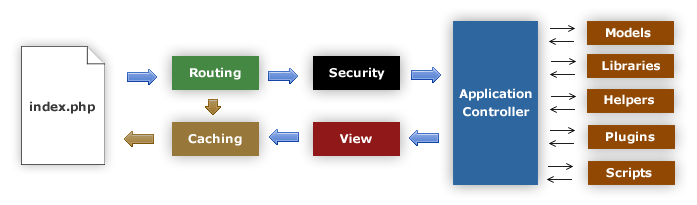
\includegraphics[width=14cm]{gambar/codeigniter}
          \caption{Alur Framework Codeigniter}
          \label{codeigniter}
      \end{figure}
    
    Gambar \ref{codeigniter} menggambarkan bagaimana data mengalir di seluruh sistem \emph{framework Codeigniter}. Kemudian deskripsi alur \emph{framework Codeigniter} dari Gambar \ref{codeigniter} adalah sebagai berikut (Hakim, 2010):
    \begin{enumerate}
      \itemsep0em
      \item Index.php yang berfungsi sebagai kontrol depan, melalui \emph{base} yang dibutuhkan untuk menjalankan \emph{Codeigniter}.
      \item \emph{Router} yang meneliti permintaan HTTP untuk menentukan apa yang harus dilakukan dengannya.
      \item Jika \emph{file cache} ada, maka langsung dikirim ke \emph{browser}.
      \item Sebelum aplikasi kontrol di ambil, maka permintaan HTTP dan pengguna mengirimkan data untuk disaring keamanannya.
      \item \emph{Controller} memanggil \emph{model, core library, plugin, helper} dan \emph{resource} lainnya yang diperlukan untuk memproses permintaan khusus.
      \item \emph{View} yang selesai kemudian dikirim ke \emph{web browser} untuk dilihat.
    \end{enumerate}

  \subsection{\emph{Unified Modeling Language} (UML)}
    \subsubsection{Definisi UML}
    UML merupakan satu kumpulan konvensi pemodelan yang digunakan untuk menentukan atau menggambarkan sebuah sistem \emph{software} yang terkait dengan obyek (Whitten, 2004). UML menawarkan diagram yang dikelompokkan menjadi beberapa perspektif berbeda untuk memodelkan suatu sistem, seperti satu set cetak biru (\emph{blueprint}) yang digunakan untuk membangun sebuah rumah (Whitten, 2004).

    \subsubsection{\emph{Use Case Diagram}}
    \emph{Use Case Diagram} merupakan diagram yang menggambarkan interaksi antara sistem dengan eksternal sistem dan pengguna. Dengan kata lain, secara grafis menggambarkan siapa yang akan menggunakan sistem dan dengan cara apa pengguna mengharapkan untuk berinteraksi dengan sistem (Whitten, 2004).

    Berikut ini merupakan pemodelan yang dimiliki oleh \emph{Use case diagram} (Whitten, 2004): \newline
    \begin{enumerate}
      \itemsep0em
      \item \emph{Use case}
      
      \emph{Use case} merupakan urutan langkah-langkah yang secara tindakan saling terkait (\emph{scenario}), baik otomatis maupun secara manual.
      \item \emph{Actor} (Pelaku)
      
      \emph{Actor} merupakan segala sesuatu yang perlu berinteraksi dengan sistem untuk pertukaran informasi.
      \item \emph{Relationship} (Hubungan)
      
      \emph{Relationship} digambarkan sebagai sebuah garis antara dua simbol. Pemaknaan \emph{relationship} berbeda-beda tergantung bagaimana garis tersebut digambar dan tipe simbol apa yang digunakan untuk menghubungkan garis tersebut. Berikut ini adalah perbedaan di antara \emph{relationship} yang ada pada sebuah diagram \emph{use case}:
        \begin{enumerate}[label=\alph*.]
          \itemsep0em
          \item \emph{Association}
          
          \emph{Association} merupakan \emph{relationship} antara \emph{actor} dengan \emph{use case} dimana terjadi interaksi di antara merekan.
          \item \emph{Extends}
          
          \emph{Extends use case} merupakan \emph{use case} yang terdiri dari langkah yang terekstrasi dari \emph{use case} yang lebih kompleks untuk menyederhanakan masalah dan karena itu memperluas fungsinya.
          \item \emph{Uses} (\emph{includes})
          
          Hubungan \emph{uses} menggambarkan bahwa satu \emph{use case} seluruhnya meliputi fungsionalitas dari \emph{use case} lainnya.
          \item \emph{Depends on}
          
          Terkadang \emph{use case} memiliki ketergantungan pada \emph{use case} lainnya yang bertujuan menentukan urutan dalam pengembangan \emph{use case}. Ketergantungan ini dimodelkan menggunakan \emph{depends on relationship}.
          \item \emph{Inheritance}
          
          Hubungan \emph{inheritance} terjadi ketika dua atau lebih \emph{actor} menggunakan \emph{use case} yang sama.
        \end{enumerate}
    \end{enumerate}

    \subsubsection{\emph{Activity Diagram}}
    \emph{Activity diagram} secara grafis digunakan untuk menggambarkan rangkaian aliran aktifitas baik proses bisnis atau \emph{use case} (Whitten, 2004).

    \subsubsection{\emph{Sequence Diagram}}
    \emph{Sequence diagram} secara grafis menggambarkan bagaimana obyek berinteraksi dengan satu sama lain melalui pesan pada eksekusi sebuah \emph{use case} atau operasi. Diagram ini mengilustrasikan bagaimana pesan terkirim dan diterima di antara obyek dan \emph{sequence} (ruang waktu) (Whitten, 2004).

    \subsubsection{\emph{Class Diagram}}
    \emph{Class Diagram} adalah gambar grafis mengenai struktur obyek statis dari suatu sistem, menunjukan kelas-kelas obyek yang menyusun sebuah sistem dan juga hubungan antara kelas obyek tersebut (Whitten, 2004).

    \subsubsection{Keunggulan UML}
    Adi Nugroho mengemukakan bahwa secara umum UML diterapkan dalam pengembangan sistem atau perangkat lunak beriontasi obyek sebab metodologi UML ini umumnya memiliki keunggulan-keunggulan sebagai berikut (Nugroho, 2005):
    \newline
    \begin{enumerate}
      \itemsep0em
      \item \emph{Uniformity}
      
      Dengan metodologi UML, para pengembang cukup menggunakan satu metodologi dari tahap analisis hingga perancangan. Hal ini tidak bisa dilakukan dalam pengembangan terstruktur. Dengan perkembangan masa kini ke arah aplikasi GUI (\emph{Graphical User Interface}), UML juga memungkinkan kita merancang komponen antar muka pengguna secara integrasi bersama dengan perancangan perangkat lunak sekaligus dengan perancangan basis data.
      \item \emph{Understandability}
      
      Dengan metodologi ini kode yang dihasilkan dapat diorganisasi ke dalam kelas-kelas yang berhubungan dengan masalah sesungguhnya sehingga lebih mudah dipahami oleh siapapun.
      \item \emph{Stability}
      
      Kode program yang dihasilkan relatif stabil sepanjang waktu sebab sangat mendekati permasalahan sesungguhnya di lapangan.
      \item \emph{Reuseability}
      
      Dengan metodologi berorientasi obyek, dimungkinkan penggunaan ulang kode, sehingga pada gilirannya akan sangat mempercepat pengembangan perangkat lunak.
    \end{enumerate}

  \subsection{\emph{Extreme Programming}}
  Permasalahan utama yang sering muncul dalam sebuah proyek pengembangan perangkat lunak adalah perubahan \emph{requirement} yang begitu cepat. Hal ini terjadi sebagai akibat perubahan-perubahan yang muncul baik pada aspek bisnis maupun teknologi yang berlangsung lebih cepat daripada proses pengembangan perangkat lunak itu sendiri. \emph{Extreme Programming} (XP) adalah sebuah pendekatan pengembangan perangkat lunak yang mencoba meningkatkan efisiensi dan fleksibilitas dari sebuah proyek pengembangan perangkat lunak dengan mengkombinasikan berbagai ide sederhana (Widhiartha, 2008).
  
    \begin{figure}[H]
        \centering
        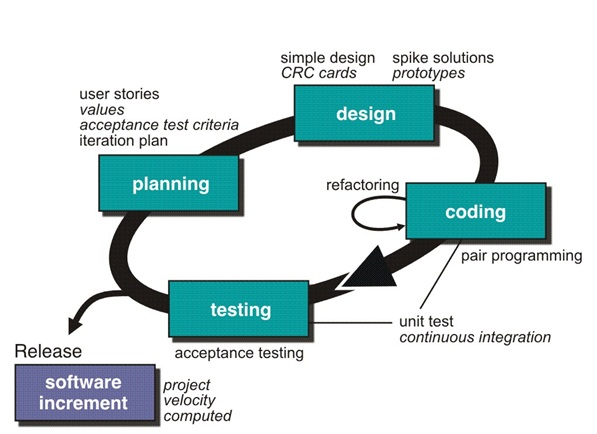
\includegraphics[width=10cm]{gambar/siklus-xp}
        \caption{Siklus \emph{Extreme Programming}}
        \label{siklus_xp}
    \end{figure}
  Menurut Sutabri (2004), \emph{Extreme Programming} terdiri dari aktifitas perencanaan (\emph{planning}), desain (\emph{design}), pengkodean (\emph{coding}), dan pengujian (\emph{testing}). Gambar \ref{siklus_xp} merupakan gambaran dari aktifitas yang ada pada \emph{Extreme Programming}, dan keterangan dari setiap tahapannya adalah sebagai berikut:
  \begin{enumerate}
      \itemsep0em
      \item \emph{Planning}
      
      Tahapan ini dimulai dengan membuat \emph{user story} (cerita) atau gambaran fitur serta fungsi dari sistem yang akan dibangun.
      \item \emph{Design}
      
      Aktifitas desain dalam pengambangan sistem bertujuan untuk merancang pola logika dalam sistem. Desain dibuat berdasarkan \emph{user story} sebelumnya.
      \item \emph{Coding}
      
      Tahap pembuatan sistem berdasarkan \emph{design} yang telah dibuat. Tahap ini dapat dilakukan secara berulang-ulang (\emph{refactoring}) apabila terdapat koreksi dari tahap berikutnya.
      \item \emph{Testing}
      
      Tahap pengujian sistem, setiap modul yang sedang dikembangkan akan terlebih dahulu mengalami pengujian. Apabila masih belum sesuai dengan permintaan maka akan dilakukan perbaikan pada bagian yang dikoreksi. Jika sudah sesuai dengan permintaan maka sistem sudah dapat diimplementasikan.
  \end{enumerate}
  \subsubsection{Nilai-nilai Dasar \emph{Extreme Programming}}
  Berikut adalah nilai-nilai mendasar yang menjadi roh dari XP pada setiap tahapan proses pengembangan perangkat lunak (Widhiartha, 2008):
  \begin{enumerate}
      \itemsep0em
      \item \emph{Communication}
      
      XP mengfokuskan pada hubungan komunikasi yang baik antar anggota tim. Para anggota tim harus membangun saling pengertian, mereka juga wajib saling berbagi pengetahuan dan keterampilan dalam mengembangkan perangkat lunak. Ego dari para programer yang biasaanya cukup tinggi harus ditekan dan mereka harus membuka diri untuk bekerjasama dengan programer lain dalam menuliskan kode program. \newline
      \item \emph{Courage}
      
      Para anggota tim dan penanggungjawab pengembangan perangkat lunak harus selalu memiliki keyakinan dan integritas dalam melakukan tugasnya. Integritas ini harus selalu dijaga bahkan dalam kondisi adanya tekanan dari situasi sekitar.
      \item \emph{Simplicity}
      
      Lakukan semua dengan sederhana. Gunakan \emph{method} yang pendek dan simpel, jangan terlalu rumit dalam membuat desain, hilangkan fitur yang tidak ada gunanya, dan berbagai proses penyederhanaan lain akan selalu menjadi nilai utama dari setiap aspek XP.
      \item \emph{Feedback}
      
      Berikan selalu \emph{feedback} kepada sesama anggota tim maupun pihak lain yang terlibat dalam pengembangan. Utarakan selalu pikiran dan diskusikan kesalahan-kesalahan yang muncul selama proses pengembangan. \emph{Feedback} inilah yang membuat kita menyadari bagian mana yang salah atau bisa ditingkatkan lagi.
      \item \emph{Quality Work}
      
      Dari ke empat nilai yang telah dijelaskan, maka akan berujung pada sebuah kondisi dimana kita melakukan pekerjaan dengan berkualitas. Dengan proses yang berkualitas maka implikasinya akan muncul pula perangkat lunak yang berkualitas sebagai hasil akhirnya.
  \end{enumerate}
  
  \subsubsection{Aspek Dasar \emph{Extreme Programming}}
  Berikut aspek dasar XP yang diterapkan (Widhiartha, 2008):
  \begin{enumerate}
      \itemsep0em
      \item \emph{Planning Game}
      
      Pendekatan XP dalam perencanaan sangat mirip dengan metode yang diterapkan pada RAD (\emph{Rapid Application Development}). Proses pendek dan cepat, mengutamakan aspek teknik, memisahkan unsur bisnis dengan unsur teknis dan pertemuan intensif antara klien dengan developer.
      \item \emph{Small Release}
      
      \emph{Release} dilakukan dalam lingkup sekecil mungkin pada XP. Setiap developer menyelesaikan sebuah unit atau bagian dari perangkat lunak maka hasil tersebut harus segera dipresentasikan dan didiskusikan dengan klien. Jika memungkinkan untuk menerapkan unit tersebut pada perusahaan, hal itu juga dapat dilakukan sekaligus sebagai tes awal dari penerapan keseluruhan sistem.
      \item \emph{Metaphor}
      
      \emph{Methapor} pada dasarnya sama dengan arsitektur perangkat lunak. Keduanya menggambarkan visi yang luas terhadap tujuan dari pengembangan perangkat lunak. Beck sendiri seperti para penandatangan Agile Manifesto lainnya bercita-cita menyederhanakan proses pengembangan perangkat lunak yang saat ini sudah dianggap terlalu rumit. \emph{Metaphor}, walaupun mirip dengan arsitektur lebih bersifat naratif dan deskriptif. Dengan demikian diharapkan komunikasi antara klien dengan developer akan berlangsung lebih baik dan lancar dengan penggunaan \emph{metaphor}.
      \item \emph{Simple Design}
      
      Sebagai salah seorang penandatangan Agile Manifesto, Beck adalah seorang yang tidak menyukai desain yang rumit dalam sebuah pengembangan perangkat lunak. Tidak heran jika dia memasukkan \emph{Simple Design} sebagai salah satu unsur XP. Pada XP desain dibuat dalam lingkup kecil dan sederhana. Tidak perlu melakukan antisipasi terhadap berbagai perubahan di kemudian hari. Dengan desain yang simpel apabila terjadi perubahan maka membuat desain baru untuk mengatasi perubahan tersebut dapat dengan mudah dilakukan dan resiko kegagalan desain dapat diperkecil.
      \item \emph{Refactoring}
      
      \emph{Refactoring} adalah salah satu aspek paling khas dari XP. \emph{Refactoring} seperti didefinisikan oleh Martin Fowler adalah "Melakukan perubahan pada kode program dari perangkat lunak dengan tujuan meningkatkan kualitas dari struktur program tersebut tanpa mengubah cara program tersebut bekerja". \emph{Refactoring} sendiri sangat sesuai untuk menjadi bagian XP karena \emph{Refactoring} mengusung konsep penyederhanaan dari proses desain maupun struktur baris kode program. Dengan \emph{Refactoring} tim pengembang dapat melakukan berbagai usaha untuk meningkatkan kualitas program tanpa kembali mengulang-ulang proses desain. Fowler adalah salah satu kolega dekat dari Kent Beck karena itu tidak mengherankan bahwa cara berpikir mereka terhadap proses pengembangan perangkat lunak sangat mirip satu dengan lainnya.
      \item \emph{Testing}
      
      XP menganut paradigma berbeda dalam hal tes dengan model pengembangan perangkat lunak lainnya. Jika pada pengembangan perangkat lunak lainnya tes baru dikembangkan setelah perangkat lunak selesai menjalani proses \emph{coding} maka pada XP tim pengembang harus membuat terlebih dahulu tes yang hendak dijalani oleh perangkat lunak. Berbagai model tes yang mengantisipasi penerapan perangkat lunak pada sistem dikembangkan terlebih dahulu. Saat proses \emph{coding} selesai dilakukan maka perangkat lunak diuji dengan model tes yang telah dibuat tersebut. Pengetesan akan jauh lebih baik apabila dilakukan pada setiap unit perangkat lunak dalam lingkup sekecil mungkin daripada menunggu sampai seluruh perangkat lunak selesai dibuat. Dengan memahami tahap ini kita dapat melihat bahwa siklus pada XP adalah \emph{requirement analysis}, \emph{test}, \emph{code}, \emph{design}. Sekilas terlihat hal ini tidak mungkin dilakukan tetapi pada kenyataannya memang gambaran inilah yang paling dapat menjelaskan tentang XP.
      \item \emph{Pair Programming}
      
      \emph{Pair programming} adalah melakukan proses menulis program dengan berpasangan. Dua orang programer saling bekerjasama di komputer yang sama untuk menyelesaikan sebuah unit. Dengan melakukan ini maka keduanya selalu dapat berdiskusi dan saling melakukan koreksi apabila ada kesalahan dalam penulisan program. Aspek ini mungkin akan sulit dijalankan oleh para programer yang memiliki ego tinggi dan sering tidak nyaman untuk berbagi komputer bersama rekannnya.
      \item \emph{Collective Ownership}
      
      Tidak ada satupun baris kode program yang hanya dipahami oleh satu orang programer. XP menuntut para programer untuk berbagi pengetahuan untuk tiap baris program bahkan beserta hak untuk mengubahnya. Dengan pemahaman yang sama terhadap keseluruhan program, ketergantungan pada programer tertentu ataupun berbagai hambatan akibat perbedaan gaya menulis program dapat diperkecil. Pada level yang lebih tinggi bahkan dimungkinkan para programer dapat bertukar unit yang dibangunnya.
      \item \emph{Coding Standards}
      
      \emph{Pair programming} dan \emph{collective ownership} hanya akan dapat berjalan dengan baik apabila para programer memiliki pemahaman yang sama terhadap penulisan kode program. Dengan adanya \emph{coding standards} yang telah disepakati terlebih dahulu maka pemahaman terhadap program akan menjadi mudah untuk semua programer dalam tim. Hal ini dapat diterapkan sebagai contoh pada penamaan variabel dan penggunaan tipe data yang sama untuk tiap elemen semua \emph{record} atau \emph{array} pada program.
      \item \emph{Continous Integrations}
      
      Melakukan build setiap hari kerja menjadi sebuah model yang disukai oleh berbagai tim pengembang perangkat lunak. Hal ini terutama didorong oleh keberhasilan penerapan sistem ini oleh \emph{Microsoft} dan telah sering dipublikasikan. Dengan melakukan \emph{build} sesering mungkin berbagai kesalahan pada program dapat dideteksi dan diperbaiki secepat mungkin. Apabila banyak tim pengembang perangkat lunak meyakini bahwa \emph{build} sekali sehari adalah maksimum maka pada XP hal tersebut adalah minimum. Pada XP tim disarankan untuk melakukan \emph{build} sesering mungkin misalnya setiap 4 jam atau bahkan lebih cepat lagi.
      \item \emph{40-hours Week}
      
      Beck berpendapat bekerja 8 jam sehari dan 5 hari seminggu adalah maksimal untuk tiap programer. Lebih dari itu programer akan cenderung membuat berbagai \emph{error} pada baris-baris kode programnya karena kelelahan.
      \item \emph{On-site Customer}
      
      Sebuah pendekatan klasik, di mana XP menganjurkan bahwa ada anggota dari klien yang terlibat pada proses pengembangan perangkat lunak. Yang lebih penting lagi ia harus ada di tempat pemrogaman dan turut serta dalam proses \emph{build} dan \emph{test} yang dilakukan. Apabila ada kesalahan dalam pengembangan diharapkan klien dapat segera memberikan masukan untuk koreksinya.
  \end{enumerate}

% Baris ini digunakan untuk membantu dalam melakukan sitasi
% Karena diapit dengan comment, maka baris ini akan diabaikan
% oleh compiler LaTeX.
\begin{comment}
\bibliography{daftar-pustaka}
\end{comment}


%!TEX root = ./template-skripsi.tex
%-------------------------------------------------------------------------------
%                            BAB III
%               		METODOLOGI PENELITIAN
%-------------------------------------------------------------------------------

\chapter{METODE PENGEMBANGAN SISTEM}
\section{Metode Pengumpulan Data}
Dalam menyelesaikan tugas akhir ini diperlukan data dan informasi sebagai bahan yang mendukung kebenaran materi dan pembahasan. Sebelum penulisan tugas akhir ini, peneliti melakukan observasi dan wawancara terlebih dahulu untuk memperoleh data serta informasi yang dibutuhkan.
    
Penulis melakukan observasi di Universitas Proklamasi 45 Yogyakarta pada bulan Maret 2018 dengan cara meninjau dan mengamati secara langsung proses penggajian yang dilakukan disana, meliputi proses pengelolaan data pegawai, rekap absensi, rekap laporan kerja pegawai, perhitungan gaji, pembuatan slip gaji dan pembayaran gaji.
    
Wawancara dilakukan dengan cara berdiskusi serta tanya jawab dengan pihak yang dapat memberikan informasi mengenai sistem penggajian yang berjalan saat ini. Beberapa pihak yang menjadi sasaran wawancara di antaranya Ibu Hartanti Widayani selaku Kepala Bagian SDM, Mbak Shofia Kurnia Putri selaku staff bagian SDM, dan Ibu Emi Eko Sulistyowati selaku Kepala Bagian Keuangan. Wawancara tersebut dilakukan pada tanggal 2 Februari 2018 dan 3 Februari 2018 bertempat di Gedung Biro Administrasi dan Umum Universitas Proklamasi 45 Yogyakarta.
    
\section{Kebutuhan Pengembangan Sistem}
    Dalam pengembangan sistem dibutuhkan perangkat keras dan perangkat lunak. Dalam penelitian ini, perangkat keras dan perangkat lunak yang digunakan adalah sebagai berikut:
	    \begin{enumerate}
	        \itemsep0em
	        \item Perangkat Keras berupa sebuah laptop dengan spesifikasi sebeagai berikut:
	            \begin{enumerate}[label=\alph*.]
	                \itemsep0em
	                \item CPU AMD A9-9420, 3.00 GHz
	                \item RAM 4 GB
	                \item VGA Radeon R5 Integrated
	            \end{enumerate}
	        \item Perangkat Lunak diantaranya sebagai berikut:
	            \begin{enumerate}[label=\alph*.]
	                \itemsep0em
	                \item Sistem Operasi Linux distro Ubuntu 18.04
	                \item XAMPP for Linux 7.25
	                \item Sublime Text Editor 3.1.1
	                \item Visual Paradigm Community Edition 15.0
	                \item Pencil Project 3.0.4
	                \item Google Chrome 67.0.3
	                \item Codeigniter 3.1.8
	            \end{enumerate}
	    \end{enumerate}

\section{Metode Pengembangan Sistem}
\subsection{\emph{Planning} (Perencanaan)}
Pada tahapan ini peneliti mendefinisikan ruang lingkup selama penelitian, menganalisis sistem yang berjalan saat ini dan permasalahan yang terjadi. Kemudian berlanjut menganalisis kebutuhan dari sistem yang akan dibangun.

\subsection{\emph{Design} (Perancangan Desain)}
Pada tahapan ini peneliti melakukan perancangan proses kerja sistem dan perancangan basis data sesuai dengan hasil pengumpulan data dan hasil analisis yang telah dilakukan. Dalam melakukan perancangan proses kerja sistem ini, peneliti menggunakan UML karena lebih menekankan pada pengembangan sistem yang berorientasi objek.
	
\subsection{\emph{Coding} (Implementasi Kode Program)}
Pada tahapan ini merupakan tahap dimana peneliti membuat sistem berdasarkan hasil desain rancangan yang telah dibuat sebelumnya. Desain rancangan diimplementasikan ke dalam bentuk kode yang dapat dipahami oleh komputer dengan bahasa pemrograman. Seperti yang telah dijelaskan sebelumnya mengenai \emph{Extreme Programming} bahwasannya metode ini melibatkan pengguna sistem dalam proses pengembangan sistem, maka proses \emph{Coding} ini dilakukan secara berulang-ulang apabila terdapat koreksi dari pengguna sistem.
	
\subsection{\emph{Testing} (Pengujian Sistem)}
Pada tahapan ini dilakukan pengujian sistem oleh pengguna sistem untuk mengatahui apakah sistem yang dikembangkan sudah sesuai dengan fungsionalitas yang diharapkan. Pada setiap proses kerja sistem dilakukan pengujian untuk mencapai hasil akhir dari tujuan sistem diperlukan terlebih dahulu proses-proses manajemen atau input data.

\chapter{ANALISIS DAN PERANCANGAN}
	
\section{\emph{Planning} (Perencanaan)}
Pada tahap \emph{planning} (perencanaan) ini yang pertama peneliti lakukan adalah mendefinisikan ruang lingkup dari penelitian ini. Kemudian melakukan analisis permasalahan terhadap sistem yang sedang berjalan dan juga menganalisis kebutuhan dari sistem yang akan dibangun.

	\subsection{Mendefinisikan Ruang Lingkup (\emph{Scope Definition})}
	Untuk lebih memfokuskan penelitian ini penulis membatasi permasalahan dan lingkup penelitian di Universitas Proklamasi 45 pada pengembangan sistem informasi penggajian karena untuk memperoleh data-data yang akurat dalam proses penggajian diperlukan pengolahan data yang optimal dan terstruktur. Perancangan sistem ini nantinya akan membantu proses pengolahan dan penyimpanan data mulai dari proses penginputan data master (data karyawan, data jabatan, data unit kerja, dan lainnya), penginputan komponen penggajian serta mempercepat perhitungan absensi agar dapat mendokumentasikan data dengan rapi dan terstruktur guna memudahkan dalam mendapatkan laporan penggajian.
		
	\subsection{Analisis Permasalahan}
	Dalam menganalisis permasalahan peneliti melakukan beberapa tahapan. Yang pertama adalah menganalisis sistem penggajian yang saat ini berjalan di Universitas Proklamasi guna mendapatkan data atau informasi mengenai bagaimana alur atau proses dalam penggajian tersebut. Yang kedua adalah mengidentifikasi permasalahan dari sistem yang saat ini berjalan. Setelah itu peneliti akan memberikan sistem usulan guna mengatasi permasalahan pada sistem yang saat ini sedang berjalan.
			
			\subsubsection{Analisis Sistem Berjalan}
				Berdasarkan hasil wawancara dan observasi yang penulis lakukan, sistem penggajian yang berjalan di Universitas Proklamasi 45 adalah sebagai berikut:
				\begin{enumerate}
					\itemsep0em
					\item Jam Kerja Karyawan
					
					Hari kerja yang diterapkan di Universitas Proklamasi 45 adalah Senin sampai dengan Sabtu, dengan total jam yaitu 40 jam per minggu. Jam kerja yang diterapkan disini tidak semua karyawan sama, tetapi terdapat beberapa tipe jam kerja, yaitu:
					\begin{enumerate}[label=\alph*.]
					    \itemsep0em
					    \item Tipe Pertama
					    
					    Hari Senin sampai Jumat, jam masuk pukul 08.00 WIB dan jam pulang pukul 16.00 WIB dengan jam istirahat selama satu jam. Untuk hari Sabtu, jam masuk pukul 08.00 WIB dan jam pulang pukul 13.00 WIB tanpa ada jam istirahat.
					    \item Tipe Kedua
					    
					    Hari Senin sampai Jumat, jam masuk pukul 10.00 WIB dan jam pulang pukul 18.00 WIB dengan jam istirahat selama satu jam. Untuk hari Sabtu, jam masuk pukul 08.00 WIB dan jam pulang pukul 13.00 WIB tanpa ada jam istirahat.
					    \item Tipe Ketiga
					    
					    Hari Senin sampai Jumat, jam masuk pukul 14.00 WIB dan jam pulang pukul 21.00 WIB dengan jam istirahat selama satu jam. Untuk hari Sabtu, jam masuk pukul 13.00 WIB dan jam pulang pukul 18.00 WIB tanpa ada jam istirahat.
					\end{enumerate}
					
					Setiap hari karyawan diwajibkan melakukan absensi fingerprint sebanyak dua kali pada waktu masuk kerja dan pulang kerja. Toleransi keterlambatan pada jam masuk kerja adalah 15 menit. Kedisiplinan karyawan dalam masuk kerja nantinya juga akan mempengaruhi besaran gaji yang akan diterima oleh setiap karyawan. Data absensi fingerprint tersimpan dalam database mesin fingerprint tersebut, akan tetapi fitur laporan absensi yang disediakan oleh mesin fingerprint tersebut belum sepenuhnya sesuai dengan kebutuhan data yang diperlukan untuk proses penggajian. Oleh karena itu staf bagian SDM perlu melakukan rekap data absensi secara manual kembali. Kegiatan rekap absensi ini dimulai setiap tanggal 21.
					\item Gaji Pokok
					
					Karyawan akan mendapatkan gaji pokok sesuai dengan perhitungan upah minimum dengan memperhatikan Undang-Undang maupun Peraturan Pemerintah. Karyawan baru yang sedang dalam masa \emph{training}, hanya akan mendapatkan 80 persen dari gaji pokok yang telah ditetapkan oleh instansi.
					\item Tunjangan dan Insentif
						\begin{enumerate}[label=\alph*.]
							\itemsep0em
							\item Tunjangan Gaji Pokok Purna Waktu
							
							Pemberian tunjangan gaji pokok purna waktu ini besaran nominalnya ditentukan oleh pihak instansi.
							\item Tunjangan Pendapatan Dini
							
							Tunjangan pendapatan dini yang dimaksud adalah pemberian tunjangan kepada karyawan dengan ketentuan yang telah ditetapkan, yaitu rata-rata absensi karyawan selama satu periode kerja minimal 35 jam. Nominal tunjangan ini sebesar Rp200.000,00.\newline
							\item Tunjangan Jabatan
							
							Karyawan yang mendapatkan tunjangan jabatan hanyalah karyawan yang memiliki jabatan tertentu, misalnya kepala unit dan kepala bidang.
							\item Insentif Operasional
							
							Insentif operasional ini besaran nominalnya masing-masing karyawan berbeda. Komponen yang mempengaruhi diantaranya adalah prestasi karyawan, kelengkapan laporan karyawan dan kedisiplinan jam datang karyawan. 
						\end{enumerate}

					\item Pendapatan Lain
						\begin{enumerate}[label=\alph*.]
							\itemsep0em
							\item Lembur
							
							Untuk mendapatkan uang dari hasil lemburnya, karyawan diharuskan untuk melakukan pengajuan lembur terlebih dahulu. Pengajuan lembur tersebut nantinya akan di review terlebih dahulu oleh Kepala Unit dari karyawan tersebut dan staf SDM sebelum disetujui.
							\item Rapat
							
							Karyawan yang menghadiri rapat akan mendapatkan upah sebesar Rp10.000,00 untuk satu kali rapat. Upah tersebut akan dibayarkan bersama dengan gaji.
							\item Pengawas Ujian
							
							Karyawan yang mendapatkan tugas atau jadwal menjadi pengawas ujian akan mendapatkan upah sebesar Rp12.500,00 untuk jam reguler dan Rp15.000,00 untuk jam malam. Upah sebagai pengawas ujian ini akan dibayarkan bersama dengan gaji. 
							\item Koreksi Ujian
							
							Karyawan yang mendapatkan tugas untuk melakukan pengoreksian hasil ujian akan mendapatkan upah sebesar Rp1.000,00 per mahasiswa. Sebagai contoh apabila mengoreksi hasil ujian 20 mahasiswa maka akan mendapatkan upah sebesar Rp.20.000,00 dan dibayarkan bersama dengan gaji.
						\end{enumerate}
				\end{enumerate}

				Staf bagian SDM mulai melakukan rekap absensi pada tanggal 21. Langkah pertama staf SDM mengambil data absensi pada mesin fingerprint, kemudian proses perekapan dilakukan menggunakan \emph{Microsoft Excel} untuk mendapatkan data akhir atau laporan absensi. Selain membuat rekap absensi, staf SDM juga membuat rekap data rapat dan data lembur karyawan. Rekap data pengawas dan korektor ujian dilakukan oleh staf bagian Akademik selaku yang bertanggung jawab masalah keakademikan, kemudian laporan rekap data tersebut akan diberikan kepada staf SDM. Setiap tanggal 21 staf SDM juga mengirimkan \emph{form} penilaian kinerja karyawan dan \emph{form} insentif operasional kepada masing-masing Kepala Unit melalui email. Selanjutnya Kepala Unit mengisi semua \emph{form} tersebut dan mengirimkannya kembali kepada staf SDM melalui email.

				Perhitungan gaji baru akan dimulai setelah pembuatan rekap seluruh data komponen gaji telah selesai dibuat, dan masih perlu dihitung secara manual. Staf Keuangan kemudian akan membuat laporan penggajian menggunakan \emph{Microsoft Excel} dan dilakukan pembuatan slip gaji masing-masing karyawan menggunakan \emph{Microsoft Excel}. Tidak ada tanggal pasti kapan proses perhitungan dan pembuatan slip gaji tersebut selesai. Dengan sistem yang berjalan saat ini, rentang waktu karyawan menerima slip gaji adalah antara tanggal 1 (satu) sampai tanggal 5 (lima). Slip gaji tersebut nantinya akan dikirimkan ke masing-masing email karyawan apabila seluruh slip gaji selesai dibuat dan disusul dengan pembayaran gaji baik melalui transfer bank ataupun melalui amplop yang dapat karyawan ambil di kantor keuangan. 

			\subsubsection{Identifikasi Masalah}
			    Dalam melakukan identifikasi masalah, peneliti perlu menganalisis sistem yang berjalan. Masalah utama yang terjadi dalam pengolahan penggajian adalah seperti kegiatan perhitungan rekap absensi, rekap data komponen penggajian, pembuatan laporan serta slip gaji yang masih bersifat manual dan menggunakan \emph{Microsoft Excel}. Hal tersebut membutuhkan tingkat ketelitian yang tinggi mengingat gaji merupakan sesuatu yang harus diterima oleh karyawan atas kerjanya untuk perusahaan dan merupakan hak masing-masing karyawan untuk menerima besaran gaji yang valid, sehingga diperlukan waktu yang cukup lama dalam proses perhitungan dan pengolahan data yang berhubungan dengan penggajian.
			    
			    Dengan tujuan membantu dan memudahkan Universitas Proklamasi 45 dalam menyelesaikan permasalahan tersebut, peneliti membangun sistem informasi penggajian yang terkomputerisasi dan terotomasi sehingga proses pengolahan data dan perhitungan gaji lebih efisien dan efektif.

			\subsubsection{Sistem Usulan}
			    Masalah utama yang dihadapi oleh Universitas Proklamasi 45 adalah masih manualnya proses rekap absensi serta perhitungan gaji karyawan yang akurat berdasar komponen-komponen gaji yang ada, sehingga sistem ini menyediakan \emph{database} yang telah dirancang untuk membantu mengatasi masalah tersebut. Data atau komponen yang menjadi syarat dan mempengaruhi perhitungan gaji terdokumentasi dengan baik dan terstruktur di dalam \emph{database} sistem. Unit atau bidang selaku pengguna sistem (\emph{users}) nantinya akan memiliki tanggung jawab masing-masing dalam mengelola dan mengolah data pada sistem ini.

		\subsection{Analisis Kebutuhan (\emph{Requirement Analysis})}
			Tahap ini mendefinisikan dan menganalisis persyaratan-persyaratan sistem yang bertujuan untuk menentukan apa saja yang dapat dilakukan oleh sistem dalam membantu dan mempercepat proses perhitungan gaji karyawan menjadi lebih efisien dan efektif.
			
			\emph{Requirements} dibagi menjadi dua bagian. Yang pertama adalah \emph{Functional Requirement} yaitu aktivitas apa yang harus disediakan oleh sistem. Kedua adalah \emph{Nonfunctional Requirement} yaitu fitur-fitur lain yang dibutuhkan oleh sistem agar lebih memuaskan pengguna dalam menggunakannya. Berikut adalah \emph{Requirement} dari sistem yang dikembangkan.

			\subsubsection{\emph{Functional Requirement}}
				\emph{Functional Requirement} yang harus dimiliki oleh sistem yang dikembangkan adalah sebagai berikut:
				\begin{enumerate}
					\itemsep0em
					\item Unit SDM (Sumber Daya Manusia)
					
						SDM menggunakan sistem ini untuk melakukan berbagai proses dan mengelola data sebagai berikut:
						\begin{enumerate}[label=\alph*.]
							\itemsep0em
							\item Data master yang meliputi data karyawan, data jabatan, data unit kerja, data periode kerja, dan data nominal komponen-komponen penggajian.
							\item Data pendapatan selain gaji pokok meliputi data rapat karyawan dan data lembur karyawan.
							\item Data absensi meliputi proses upload absensi dan mengelola permintaan absensi susulan karyawan.
							\item Data laporan kerja karyawan meliputi Rencana Kerja Harian, Laporan Harian, Checklist Bulanan dan Laporan Bulanan.
						\end{enumerate}
					\item Bidang Akademik
					
						Bidang Akademik menggunakan sistem ini untuk mengelola data sebagai berikut:
						\begin{enumerate}[label=\alph*.]
							\itemsep0em
							\item Data keakademikan meliputi data fakultas, data program studi dan data mata kuliah.
							\item Data ujian meliputi input data UTS dan data UAS.
							\item Data pendapatan selain gaji pokok meliputi data pengawas ujian dan data korektor ujian.
							\item Data pendapatan dosen selain gaji pokok meliputi tunjangan SKS dan transport mengajar.
						\end{enumerate}
					\item Bidang Keuangan
					
						Keuangan menggunakan sistem ini untuk melakukan proses \emph{generate} gaji karyawan setelah data komponen penggajian terselesaikan oleh unit SDM dan bidang Akademik. Keuangan juga dapat melihat laporan penggajian karyawan guna keperluan pendokumentasian data.
					\item Pimpinan
					
						Pimpinan menggunakan sistem ini untuk melakukan beberapa tindakan diantaranya melihat laporan penggajian karyawan, melihat penilaian kinerja karyawan guna menjadi bahan evaluasi karyawan.
					\item Karyawan
					
						Karyawan menggunakan sistem ini untuk melakukan beberapa proses sebagai berikut:
						\begin{enumerate}[label=\alph*.]
							\itemsep0em
							\item Melihat data komponen penggajian meliputi data, absensi, data lembur, data rapat, data pengawas dan koreksi ujian, serta data penilaian kinerja.
							\item Melakukan pengajuan yang meliputi pengajuan lembur dan pengajuan absensi susulan.
							\item Mengisi data laporan kerja meliputi Rencana Kerja Harian, Laporan Kerja Harian, Checklist Bulanan dan Laporan Kerja Bulanan.
						\end{enumerate}
					\item Kepala Unit
					
					    Kepala Unit menggunakan sistem ini untuk melakukan beberapa proses sebagai berikut:
					    \begin{enumerate}[label=\alph*.]
					        \itemsep0em
					        \item Melakukan \emph{input} penilaian kinerja karyawan yang dibawahinya.
					        \item Memberikan insentif operasional kepada karyawan yang dibawahinya.
					        \item Melihat data laporan kerja karyawan.
					    \end{enumerate}
				\end{enumerate}

			\subsubsection{\emph{Nonfunctional Requirement}}
				\emph{Nonfunctional Requirement} yang harus dimiliki oleh sistem dapat dilihat pada tabel \ref{nonfunctional_requirement}.
				\begin{spacing}{1.25}
                \begin{longtable}{|p{3cm}|p{10cm}|}
                \caption{\emph{Nonfunctional Requirement}}
                \label{nonfunctional_requirement} \\
                
                \hline \multicolumn{1}{|c|}{\textbf{Kebutuhan}} & \multicolumn{1}{c|}{\textbf{Penjelasan}}  \\ \hline 
                \endfirsthead
                
                \multicolumn{2}{c}%
                {{\bfseries \tablename\ \thetable{}: }\emph{Nonfunctional Requirement} (lanjutan)} \\
                \hline \multicolumn{1}{|c|}{\textbf{Kebutuhan}} &
                \multicolumn{1}{c|}{\textbf{Penjelasan}} \\ \hline 
                \endhead
                \hline
                \endfoot
                
                \hline \hline
                \endlastfoot
                {\emph{Service}} & Kemudahan dalam menggunakan sistem dan manajemen data dalam sistem  \\ \hline
                \emph{Performance} & \emph{Interface} yang \emph{user friendly}  \\ \hline
                \multirow{4}{*}{\emph{Information}} & Mencegah hilangnya data-data penggajian  \\ 
                & Mencegah \emph{redundancy} data ketika proses pengolahan data \\
                & Format laporan mudah dipahami \\
                & Data terdokumentasi dan terstruktur dengan baik \\ \hline
                \emph{Control} & Dalam melakukan tindakan dalam sistem, Actor memiliki wewenang masing-masing sesuai levelnya  \\ \hline
                \emph{Accuracy} & Proses pengolahan dan perhitungan gaji dilakukan oleh sistem sehingga hasil lebih akurat  \\ \hline
                \emph{Efficiency} & Efisiensi waktu rekap absensi dan perhitungan gaji serta efisiensi waktu dalam penyediaan laporan ketika dibutuhkan dengan cepat \\ \hline
                \emph{Effectiveness} & Proses penggajian langsung pada sistem yang terkomputerisasi dan menghasilkan \emph{output} sesuai yang diharapkan \\ \hline
                \end{longtable}
                \end{spacing}
			    \vspace{2mm}
	\section{\emph{Design} (Perancangan)}
	Pada tahap ini peneliti melakukan perancangan proses atau pola logika dalam sistem yang akan dibangun. Kemudian berlanjut melakukan perancangan basis data dan juga \emph{user interface}.

		\subsection{Perancangan Proses}
			Peneliti menggunakan UML (\emph{Unified Modeling Language}) dalam melakukan perancangan proses Sistem Informasi Penggajian. Alasan memilih menggunakan UML adalah karena UML berfokus pada pendekatan sistem berorientasi objek yang terdiri dari \emph{use case diagram}, \emph{activity diagram}, \emph{sequence diagram} dan \emph{class diagram} dengan menggunakan \emph{tool} \emph{Visual Paradigm Community Edition}.
			
			\subsubsection{\emph{Use Case Diagram}}
			    Pembuatan \emph{Use Case Diagram} bertujuan untuk menggambarkan interaksi antara sistem dan pengguna. Pertama peneliti mengidentifikasi aktor, kemudian mengidentifikasi \emph{use case}.\newline
			    \begin{enumerate}
			        \itemsep0em
			        \item Identifikasi Aktor
			        
			        Pada pembuatan \emph{Use Case}, sebelumnya peneliti melakukan identifikasi aktor yang akan menggunakan sistem yang dikembangkan. Detail mengenai identifikasi aktor dapat dilihat pada Tabel \ref{actor}.
			        \begin{spacing}{1.25}
			        \begin{longtable}{|p{1cm}|p{3cm}|p{8cm}|}
			            \caption[Identifikasi Aktor.]{Identifikasi Aktor.} \label{actor} \\
                        \hline \textbf{No.} & \textbf{Aktor} & \textbf{Hak Akses}  \\ \hline 
                        \endfirsthead
                        
                        \multicolumn{3}{c}%
                        {{\bfseries \tablename\ \thetable{}:} Identifikasi Aktor (lanjutan)} \\
                        \hline \textbf{No.} & \textbf{Aktor} & \textbf{Hak Akses}  \\ \hline
                        \endhead
                        \hline
                        \endfoot
                        \hline \hline
                        \endlastfoot
                        
                        1. & SDM & Aktor yang mempunyai wewenang dalam manajemen data karyawan, unit kerja dan jabatan, status kepegawaian karyawan, lembur, rapat, periode kerja serta absensi \\ \hline
                        2. & Akademik & Aktor yang mempunyai wewenang dalam manajemen data ujian, pengawas dan korektor dari masing-masing ujian \\ \hline
                        3. & Keuangan & Aktor yang bertugas melakukan \emph{generate} slip gaji dan mencetak laporan penggajian \\ \hline
                        4. & Pimpinan & Aktor yang mempunyai wewenang dalam melihat laporan penggajian karyawan \\ \hline
                        5. & Kepala Unit & Aktor yang mempunyai wewenang dalam memberikan penilaian kinerja kepada karyawan \\ \hline
                        6. & Karyawan & Aktor yang memiliki akses untuk melihat data absensi, rapat, lembur, pengawas ujian, penilaian kerja dan membuat laporan kerja, serta mencetak slip gaji \\ \hline
			        \end{longtable}
			        \end{spacing}
			        \vspace{4mm}
			        \item Identifikasi \emph{Use Case}
			        
			        Setelah melakukan indentifikasi aktor, selanjutnya peneliti melakukan identifikasi \emph{Use Case} dari masing-masing aktor. Detail dari identifikasi \emph{Use Case} dapat dilihat pada Tabel \ref{indentifikasi_usecase}.
			        \begin{spacing}{1.25}			        \begin{longtable}{|>{\centering}p{1.5em}|>{\raggedright}p{3.5cm}|>{\raggedright}p{5.5cm}|p{2cm}|}
			            \caption{Identifikasi \emph{Use Case}} 
			            \label{indentifikasi_usecase} \\
                        \hline \textbf{No.} & \textbf{Nama \emph{Use Case}} & \textbf{Deskripsi} & \textbf{Aktor}  \\ \hline 
                        \endfirsthead
                        
                        \multicolumn{4}{c}%
                        {{\bfseries \tablename\ \thetable{}: }Identifikasi \emph{Use Case} (lanjutan)} \\
                        \hline \textbf{No.} & \textbf{Nama \emph{Use Case}} & \textbf{Deskripsi} & \textbf{Aktor}  \\ \hline
                        \endhead
                        \hline
                        \endfoot
                        \hline \hline
                        \endlastfoot
                        
                        1. & \emph{Login} & Menjelaskan bagaimana proses \emph{users} masuk ke dalam sistem & Semua aktor \\ \hline
                        2. & Manajemen data karyawan & Menjelaskan bagaimana proses tambah, edit dan hapus data karyawan & SDM \\ \hline
                        3. & Manajemen data unit kerja & Menjelaskan bagaimana proses tambah, edit dan hapus data unit kerja & SDM \\ \hline
                        4. & Manajemen data jabatan & Menjelaskan bagaimana proses tambah, edit dan hapus data jabatan & SDM \\ \hline
                        5. & Manajemen posisi dan jabatan kerja karyawan & Menjelaskan bagaimana proses mutasi karyawan dari unit yang satu ke unit yang lainnya & SDM \\ \hline
                        6. & Manajemen status kepegawaian karyawan & Menjelaskan bagaimana proses pengubahan status kepegawaian karyawan & SDM \\ \hline
                        7. & Manajemen nominal komponen penggajian & Menjelaskan bagaimana proses input data periode kerja karyawan & SDM \\ \hline
                        8. & Input data periode kerja & Menjelaskan bagaimana proses input data periode kerja karyawan & SDM \\ \hline
                        9. & Input data rapat & Menjelaskan bagaimana proses input data rapat & SDM \\ \hline
                        10. & Input data lembur & Menjelaskan bagaimana proses input data lembur karyawan & SDM \\ \hline
                        11. & \emph{Upload} absensi & Menjelaskan bagaimana proses \emph{upload} data absensi ke dalam sistem & SDM \\ \hline
                        12. & Input data ujian & Menjelaskan bagaimana proses input data ujian baik UTS maupun UAS & Akademik \\ \hline
                        13. & Input data pengawas ujian & Menjelaskan bagaimana proses input data pengawas ujian & Akademik \\ \hline
                        14. & Input data korektor ujian & Menjelaskan bagaimana proses input data korektor ujian & Akademik \\ \hline
                        15. & Lihat absensi & Menampilkan data absensi karyawan & SDM, karyawan \\ \hline
                        16. & Lihat data rapat & Menampilkan data kehadiran rapat karyawan & SDM, karyawan \\ \hline
                        17. & Lihat data lembur & Menampilkan data lembur karyawan & SDM, karyawan \\ \hline
                        18. & Lihat data pengawas ujian & Menampilkan data karyawan pengawas ujian & Akademik, karyawan \\ \hline
                        19. & Lihat data korektor ujian & Menampilkan data karyawan yang menjadi korektor ujian & Akademik, karyawan \\ \hline
                        20. & Input laporan kerja & Menjelaskan proses input laporan kerja karyawan baik harian maupun bulanan & Karyawan \\ \hline
                        21. & Lihat laporan kerja & Menampilkan laporan kerja dari karyawan & SDM, Kepala unit \\ \hline
                        22. & Input penilaian kinerja karyawan & Menjelaskan proses pemberian nilai kinerja karyawan & Kepala Unit \\ \hline
                        23. & Input insentif operasional karyawan & Menjelaskan proses penginputan jumlah insentif operasional karyawan untuk setiap periode & Kepala unit \\ \hline
                        24. & Lihat data penilaian kinerja & Menampilkan data penilaian kinerja karyawan & Karyawan \\ \hline
                        25. & \emph{Generate} slip gaji & Menjelaskan proses pembuatan slip gaji karyawan & Keuangan \\ \hline
                        26. & Cetak slip gaji & Mencetak slip gaji sesuai dengan periode kerja & Keuangan, karyawan \\ \hline
                        27. & Lihat laporan penggajian & Menampilkan laporan penggajian karyawan & Pimpinan \\ \hline
			        \end{longtable}
			        \end{spacing}
			        \vspace{4mm}
			        \newpage
			        \item Penggambaran \emph{Use Case Diagram}
			        
			        Setelah melakukan identifikasi aktor dan identifikasi \emph{use case}, peneliti merancang \emph{use case diagram} sebagaimana dapat dilihat pada Gambar \ref{usecase}.
			        \begin{figure}[H]
    		            \centering    		            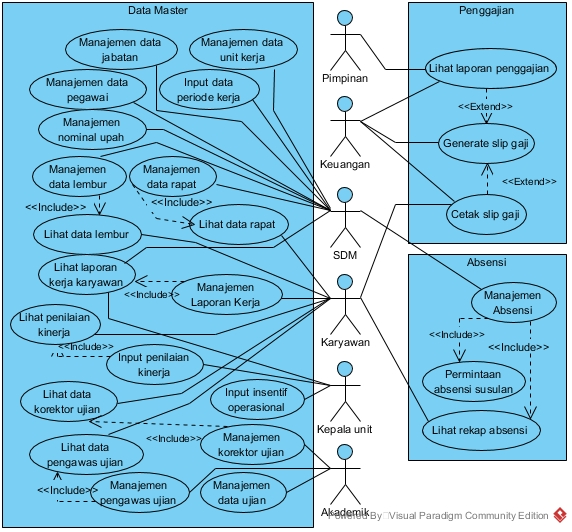
\includegraphics[width=15cm]{gambar/use-case-diagram}
    		            \caption{\emph{Use Case Diagram}}
    		            \label{usecase}
    		            \end{figure}
    			    \end{enumerate}
			        
			
			\subsubsection{\emph{Activity Diagram}}
			Berikut adalah perancangan \emph{activity diagram} yang peneliti lakukan dalam menggambarkan aktivitas masing-masing aktor dalam Sistem Informasi Penggajian Universitas Proklamasi 45:
			\begin{enumerate}
			    \itemsep0em
			    \item \emph{Activity Diagram Login}
			        \begin{figure}[H]
            		    \centering            		    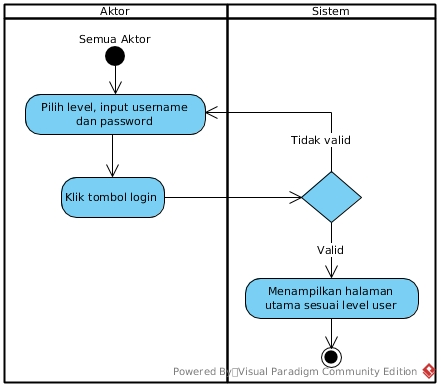
\includegraphics[width=13cm]{gambar/activity/login-activity}
            		    \caption{\emph{Activity Diagram Login}}
            		    \label{activity_login}
            		\end{figure}
            		\emph{Activity Diagram} pada Gambar \ref{activity_login} menjelaskan bagaimana aktor masuk ke dalam sistem. Pada halaman \emph{Login}, aktor akan memilih level \emph{user}, memasukan \emph{Username} dan \emph{Password}. Kemudian sistem akan melakukan validasi data. Apabila data valid, sistem akan menampilkan halaman Dashboard. Sedangkan apabila data yang dimasukan tidak valid, sistem akan kembali ke halaman \emph{Login} dan menampilkan pesan kesalahan.\newpage
			    \item \emph{Activity Diagram} Manajemen Data Karyawan
			        \begin{figure}[H]
            		    \centering            		    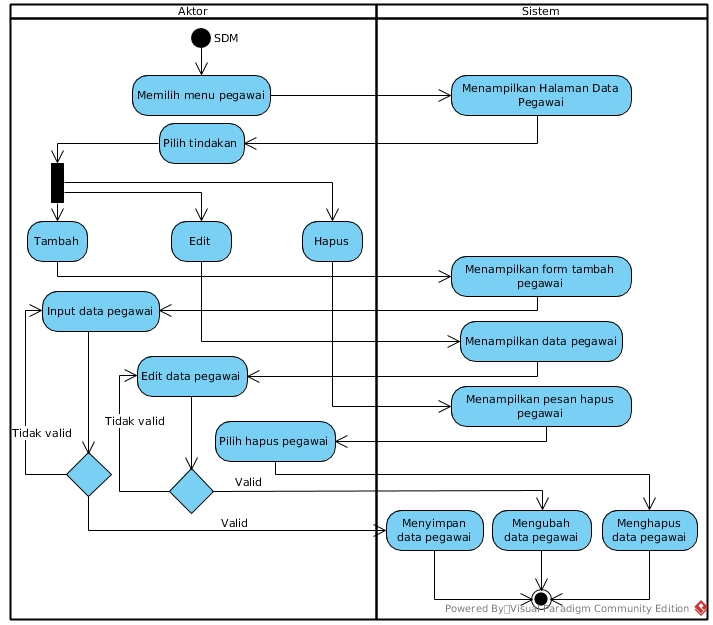
\includegraphics[width=14cm]{gambar/activity/manajemen-data-pegawai}
            		    \caption{\emph{Activity Diagram} Manajemen Data Karyawan}
            		    \label{activity_manajemen_pegawai}
            		\end{figure}
            		\emph{Activity Diagram} pada Gambar \ref{activity_manajemen_pegawai} menjelaskan bagaimana SDM melakukan manajemen data karyawan. Langkah pertama adalah memilih menu data karyawan dan sistem akan menampilkan halaman data karyawan. Manajemen data karyawan yang dimaksud adalah proses menambah, mengubah serta menghapus data karyawan. Ketika memilih tindakan tambah data karyawan, sistem akan menampilkan \emph{form} penambahan data yang berisi \emph{input field} yang harus diisi oleh SDM. Dalam melakukan tindakan tambah dan edit data karyawan, data akan divalidasi oleh sistem sebelum data disimpah atau diubah ke dalam \emph{database}.\newpage
            	\item \emph{Activity Diagram} Manajemen Data Unit Kerja
			        \begin{figure}[H]
            		    \centering            		     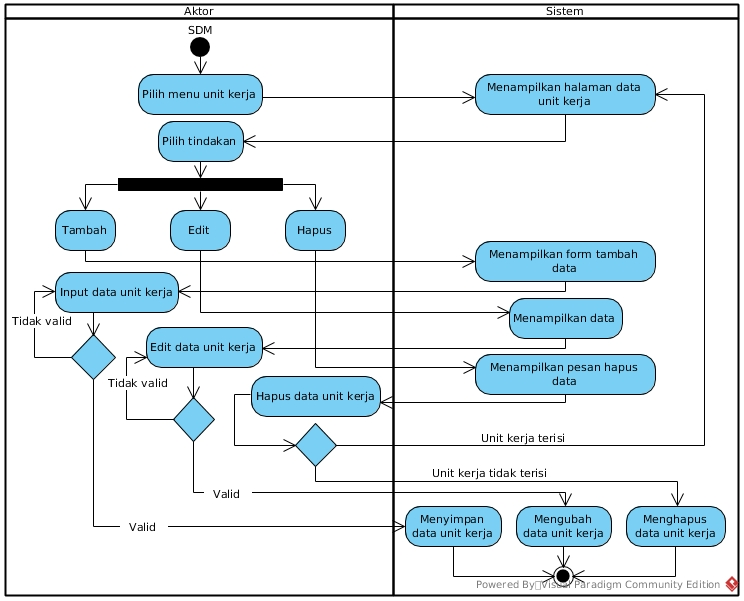
\includegraphics[width=14cm]{gambar/activity/manajemen-unit-kerja}
            		    \caption{\emph{Activity Diagram} Manajemen Unit Kerja}
            		    \label{activity_manajemen_unit}
            		\end{figure}
            		Dalam sebuah perusahaan pastinya perlu adanya bidang-bidang atau unit kerja yang mempunyai ranah kerja masing-masing. \emph{Activity Diagram} pada Gambar \ref{activity_manajemen_unit} menjelaskan bagaimana SDM melakukan manajemen data unit kerja karyawan, Pada setiap proses menambah data, mengubah data dan menghapus data unit kerja, sistem akan melakukan validasi data terlebih dahulu sebelum memproses tindakan tersebut. Seperti ketika ingin menghapus data unit kerja, apabila unit kerja terisi oleh karyawan, maka sistem akan membatalkan proses penghapusan tersebut. \newpage
            	\item \emph{Activity Diagram} Manajemen Data Jabatan
			        \begin{figure}[H]
            		    \centering
            		    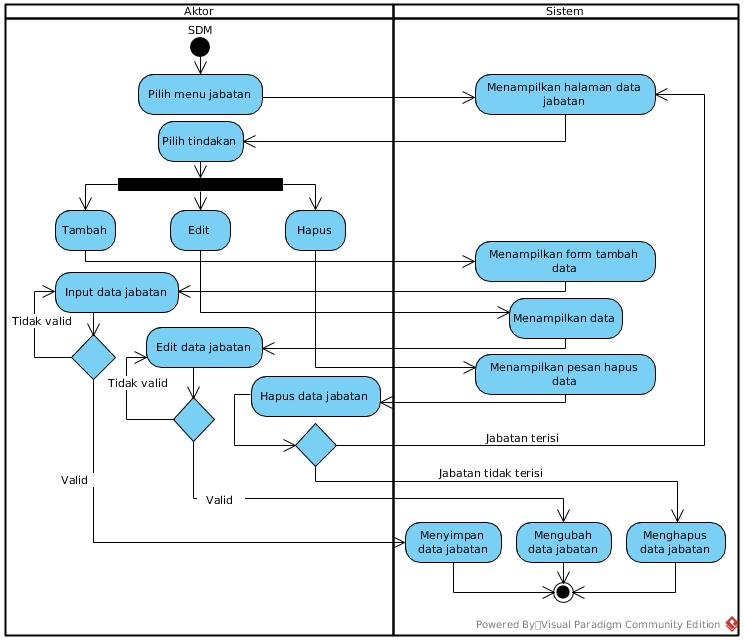
\includegraphics[width=14cm]{gambar/activity/manajemen-data-jabatan}
            		    \caption{\emph{Activity Diagram} Manajemen Data Jabatan}
            		    \label{activity_manajemen_jabatan}
            		\end{figure}
            		\emph{Activity Diagram} pada Gambar \ref{activity_manajemen_jabatan} menjelaskan bagaimana SDM melakukan manajemen data jabatan. Pada setiap proses menambah data, mengubah data dan menghapus data jabatan, sistem akan melakukan validasi data terlebih dahulu sebelum memproses tindakan tersebut. Seperti ketika ingin menghapus data jabatan, apabila jabatan tersebut terisi oleh karyawan, maka sistem akan membatalkan proses penghapusan tersebut. \newpage
            	\item \emph{Activity Diagram} Managemen Status Kepegawaian Pegawai
            	    \begin{figure}[H]
            		    \centering
            		    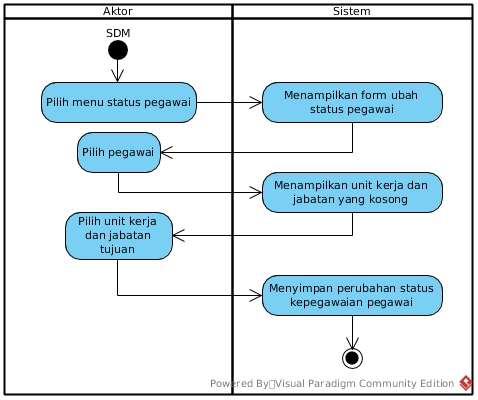
\includegraphics[width=14cm]{gambar/activity/manajemen-status-pegawai}
            		    \caption{\emph{Activity Diagram} Manajemen Status Kepegawaian Pegawai}
            		    \label{activity_status_pegawai}
            		\end{figure}
            		\emph{Activity Diagram} pada Gambar \ref{activity_status_pegawai} menjelaskan bagaimana proses SDM melakukan perubahan status kepegawaian pegawai, dalam hal ini unit kerja dan jabatan pegawai. SDM memilih menu status pegawai dan sistem akan menampilkan form ubah status pegawai. Kemudian SDM memilih pegawai yang akan diubah status kepegawaiannya dan sistem akan menampilkan data unit kerja dan jabatan yang kosong. SDM memilih unit kerja dan jabatan tujuan kemudian sistem akan menyimpan perubahan status kepegawaian pegawai tersebut. \newpage
            	\item \emph{Activity Diagram} Input Data Periode Kerja
            	    \begin{figure}[H]
            		    \centering
            		    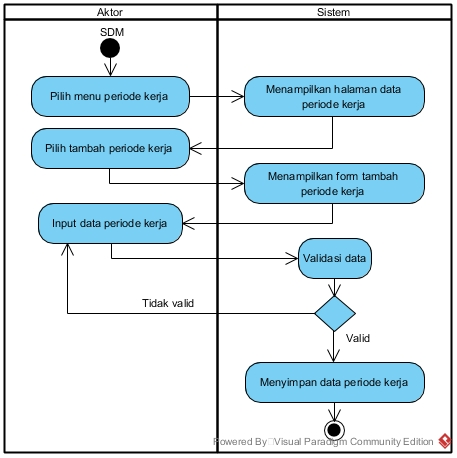
\includegraphics[width=13cm]{gambar/activity/input-data-periode-kerja}
            		    \caption{\emph{Activity Diagram} Input Data Periode Kerja}
            		    \label{activity_periode_kerja}
            		\end{figure}
            		\emph{Activity Diagram} pada Gambar \ref{activity_periode_kerja} menjelaskan bagaimana SDM melakukan \emph{input} data periode kerja. Pertama SDM akan memilih menu periode kerja dan sistem akan menampilkan halaman data periode kerja. Kemudian SDM memilih tindakan tambah periode kerja dan sistem akan menampilkan \emph{form} tambah periode kerja. Pada \emph{form} tersebut SDM mengisikan data-data periode kerja. Sebelum data periode kerja disimpan, sistem akan melakukan validasi data tersebut terlebih dahulu. \newpage
            	\item \emph{Activity Diagram} Manajemen Data Rapat
            	
            	Dalam proses manajemen data rapat terdapat beberapa \emph{activity} yang meliputi input data rapat, rekap upah rapat, dan lihat data rapat. Detail dari masing-masing \emph{activity} tersebut adalah sebagai berikut:
            	\begin{enumerate}[label=\alph*.]
            	    \itemsep0em
            	    \item Input Data Rapat
            	    \begin{figure}[H]
            		    \centering            		    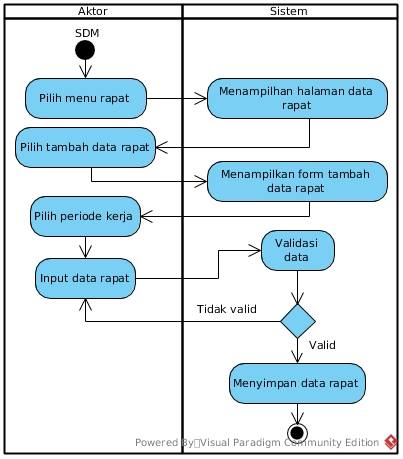
\includegraphics[width=11cm]{gambar/activity/input-data-rapat}
            		    \caption{\emph{Activity Diagram} Input Data Rapat}
            		    \label{activity_input_rapat}
            		\end{figure}
            		\emph{Activity Diagram} pada Gambar \ref{activity_input_rapat} menjelaskan bagaimana SDM melakukan penambahan data rapat karyawan. SDM memilih menu rapat dan sistem akan menampilkan halaman data rapat. Ketika memilih tambah data rapat, sistem akan menampilkan \emph{form} tambah data rapat. Kemudian SDM mengisi data rapat dan sistem akan melakukan validasi sebelum data disimpan.
            		\item Rekap Upah Rapat
            		\begin{figure}[H]
            		    \centering            		    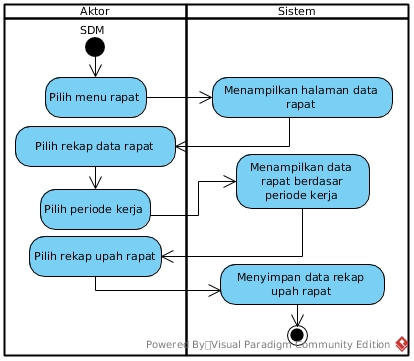
\includegraphics[width=11cm]{gambar/activity/rekap-upah-rapat}
            		    \caption{\emph{Activity Diagram} Rekap Upah Rapat}
            		    \label{activity_rekap_rapat}
            		\end{figure}
            		\emph{Activity Diagram} pada Gambar \ref{activity_rekap_rapat} menjelaskan bagaimana proses SDM melakukan perekapan upah rapat karyawan. Pada halaman data rapat SDM memilih rekap data rapat, lalu memilih periode kerja. Sistem akan menampilkan data rapat berdasarkan periode kerja yang dipilih. Setelah itu SDM dapat melakukan perekapan upah rapat selama satu periode yang dipilih.\newpage
            		\item Lihat Data Rapat
            		\begin{figure}[H]
            		    \centering            		    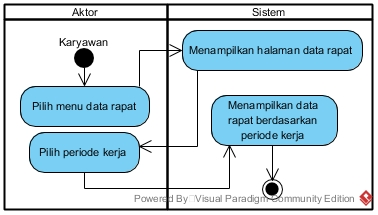
\includegraphics[width=11cm]{gambar/activity/lihat-data-rapat}
            		    \caption{\emph{Activity Diagram} Lihat Data Rapat}
            		    \label{activity_lihat_rapat}
            		\end{figure}
            		\emph{Activity Diagram} pada Gambar \ref{activity_lihat_rapat} menjelaskan bagaimana proses karyawan melihat data rapat yang dihadirinya. Pertama karyawan memilih menu data rapat dan sistem akan menampilkan halaman data rapat. Karyawan kemudian memilih periode kerja terlebih dahulu. Setelah itu sistem akan menampilkan data rapat karyawan sesuai dengan periode kerja yang dipilih.
            	\end{enumerate}
            	
            	\item \emph{Activity Diagram} Manajemen Data Lembur
            	
            	Dalam proses manajemen data lembur karyawan terdapat beberapa \emph{activity} yang meliputi input data lembur, rekap upah lembur, dan lihat data lembur. Detail dari masing-masing \emph{activity} tersebut adalah sebagai berikut: \newpage
            	\begin{enumerate}[label=\alph*.]
            	    \itemsep0em
            	    \item Input Data Lembur
            	    \begin{figure}[H]
            		    \centering            		    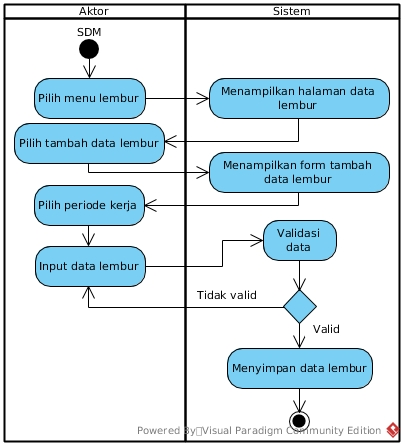
\includegraphics[width=11cm]{gambar/activity/input-data-lembur}
            		    \caption{\emph{Activity Diagram} Input Data Lembur}
            		    \label{activity_input_lembur}
            		\end{figure}
            		\emph{Activity Diagram} pada Gambar \ref{activity_input_lembur} menjelaskan bagaimana proses SDM melakukan penambahan data lembur karyawan. SDM memilih menu lembur dan sistem akan menampilkan halaman data lembur. Ketika SDM memilih tambah data lembur, sistem akan menampilkan \emph{form} tambah data lembur. Kemudian SDM memilih periode kerja dan mengisi data lembur. Setelah itu sistem akan melakukan validasi sebelum data lembur tersebut disimpan.\newpage
            	    \item Rekap Upah Lembur
            	    \begin{figure}[H]
            		    \centering            		    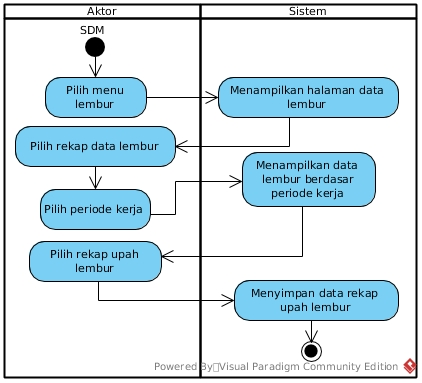
\includegraphics[width=11cm]{gambar/activity/rekap-upah-lembur}
            		    \caption{\emph{Activity Diagram} Rekap Upah Lembur}
            		    \label{activity_rekap_lembur}
            		\end{figure}
            		\emph{Activity Diagram} pada Gambar \ref{activity_rekap_lembur} menjelaskan bagaimana proses SDM melakukan perekapan upah lembur karyawan. Pada halaman data lembur SDM memilih rekap data lembur. Kemudian SDM memilih periode kerja dan sistem akan menampilkan data lembur karyawan berdasarkan periode kerja yang dipilih. Setelah itu SDM dapat melakukan perekapan upah lembur karyawan selama satu periode yang dipilih.\newpage
            	    \item Lihat Data Lembur
            	    \begin{figure}[H]
            		    \centering            		    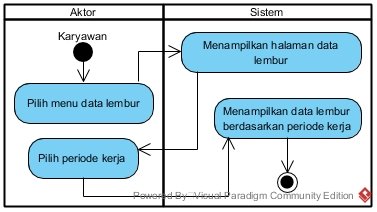
\includegraphics[width=11cm]{gambar/activity/lihat-data-lembur}
            		    \caption{\emph{Activity Diagram} Lihat Data Lembur}
            		    \label{activity_lihat_lembur}
            		\end{figure}
            		\emph{Activity Diagram} pada Gambar \ref{activity_lihat_lembur} menjelaskan bagaimana proses karyawan melihat data lembur yang dilakukannya. Pertama karyawan memilih menu data lembur dan sistem akan menampilkan halaman data lembur. Karyawan kemudian memilih periode kerja terlebih dahulu. Setelah itu sistem akan menampilkan data lembur karyawan sesuai dengan periode kerja yang dipilih.
            	\end{enumerate}
            	    
            	\item \emph{Activity Diagram} Manajemen Data Absensi
            	
            	Dalam proses manajemen data absensi karyawan terdiri dari beberapa \emph{activity} yang meliputi \emph{upload} data absensi dan ubah data absensi yang dapat dilakukan oleh SDM, serta lihat data absensi yang dapat dilakukan oleh karyawan. Detail dari masing-masing \emph{activity} tersebut adalah sebagai berikut: \newpage
            	\begin{enumerate}[label=\alph*.]
            	    \itemsep0em
            	    \item \emph{Upload} Data Absensi
            	    \begin{figure}[H]
            		    \centering            		    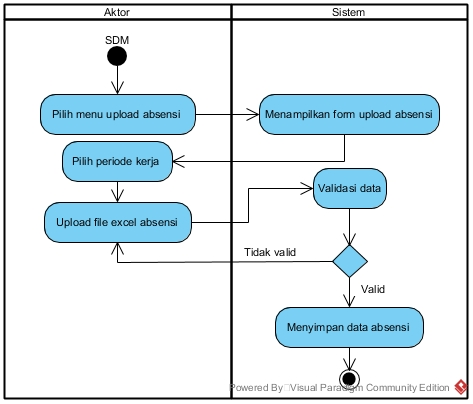
\includegraphics[width=13cm]{gambar/activity/upload-absensi}
            		    \caption{\emph{Activity Diagram} Upload Absensi}
            		    \label{activity_upload_absensi}
            		\end{figure}
            		\emph{Activity Diagram} pada Gambar \ref{activity_upload_absensi} menjelaskan bagaimana SDM melakukan proses \emph{upload} atau pengunggahan data absensi karyawan. SDM memilih tindakan \emph{upload} absensi dan sistem akan menampilkan \emph{form upload} absensi. Sebelum memilih file, SDM terlebih dahulu memilih periode kerja sesuai dengan periode kerja yang sedang berjalan. Sistem akan melakukan validasi terlebih dahulu sebelum data absensi tersebut disimpan.\newpage
            	    \item Ubah Data Absensi
            	    \begin{figure}[H]
            		    \centering            		    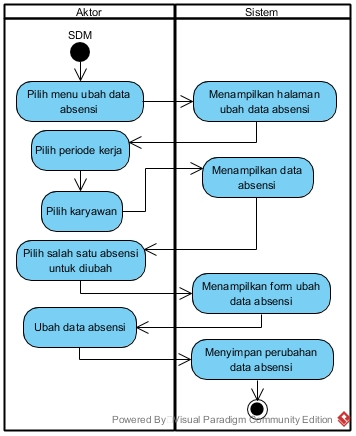
\includegraphics[width=11cm]{gambar/activity/ubah-data-absensi}
            		    \caption{\emph{Activity Diagram} Ubah Data Absensi}
            		    \label{activity_ubah_absensi}
            		\end{figure}
            		\emph{Activity Diagram} pada Gambar \ref{activity_ubah_absensi} menjelaskan bagaimana proses SDM melakukan perubahan data absensi karyawan. SDM memilih menu ubah data absensi dan sistem akan menampilkan halaman ubah data absensi. Kemudian SDM memilih karyawan dan periode kerja. Setelah itu sistem akan menampilkan data absensi sesuai karyawan dan periode yang dipilih. SDM memilih salah satu data absensi yang akan dilakukan perubahan. Sistem akan menampilkan \emph{form} ubah data absensi. Setelah itu SDM dapat mengubah data absensi yang dipilih dan sistem akan menyimpan perubahan data absensi tersebut.
            	    \item Lihat Rekap Absensi
            	    \begin{figure}[H]
            		    \centering            		    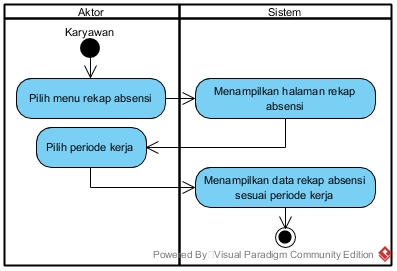
\includegraphics[width=11cm]{gambar/activity/lihat-data-rekap-absensi}
            		    \caption{\emph{Activity Diagram} Lihat Data Rekap Absensi}
            		    \label{activity_lihat_absensi}
            		\end{figure}
            		\emph{Activity Diagram} pada Gambar \ref{activity_lihat_absensi} menjelaskan bagaimana proses karyawan melihat data rekap absensi. Karyawan memilih menu data rekap absensi dan sistem akan menampilkan halaman rekap absensi. Kemudian karyawan memilih periode kerja terlebih dahulu. Setelah itu sistem akan menampilkan data rekap absensi karyawan tersebut sesuai periode kerja yang dipilih.
            	\end{enumerate}
            	    
            	\item \emph{Activity Diagram} Manajemen Data Ujian
            	
            	Dalam proses manajemen data ujian terdapat beberapa \emph{activity} yang meliputi input data ujian, input pengawas ujian, input korektor ujian, rekap upah pengawas ujian, rekap upah korektor ujian, lihat data pengawas ujian dan lihat data korektor ujian. Detail dari masing-masing \emph{activity} tersebut adalah sebagai berikut: \newpage
            	\begin{enumerate}[label=\alph*.]
            	    \itemsep0em
            	    \item Input Data Ujian
            	    \begin{figure}[H]
            		    \centering            		    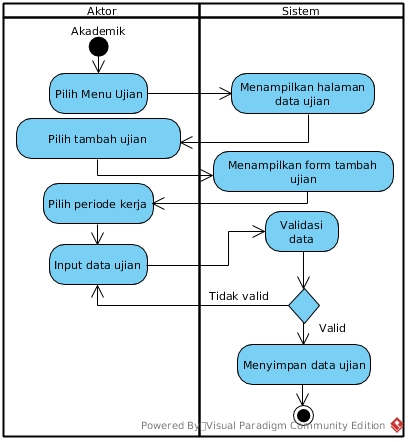
\includegraphics[width=11cm]{gambar/activity/input-data-ujian}
            		    \caption{\emph{Activity Diagram} Input Data Ujian}
            		    \label{activity_input_ujian}
            		\end{figure}
            		\emph{Activity Diagram} pada Gambar \ref{activity_input_ujian} menjelaskan bagaimana staf Akademik melakukan \emph{input} data ujian. Staf Akademik memilih menu ujian dan sistem menampilkan halaman data ujian. Ketika memilih tambah ujian, sistem akan menampilkan form tambah data ujian. Staf akademik memilih periode kerja dan mengisi data ujian, kemudian sistem akan melakukan validasi sebelum data disimpan ke dalam \emph{database}.\newpage
            		\item Input Data Pengawas Ujian
            		\begin{figure}[H]
            		    \centering            		    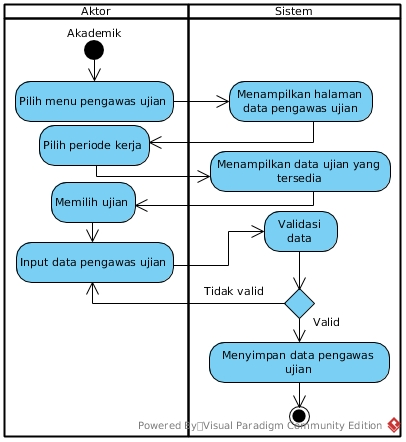
\includegraphics[width=11cm]{gambar/activity/input-data-pengawas-ujian}
            		    \caption{\emph{Activity Diagram} Input Data Pengawas Ujian}
            		    \label{activity_input_pengawas}
            		\end{figure}
            		\emph{Activity Diagram} pada Gambar \ref{activity_input_pengawas} menjelaskan bagaimana staf Akademik melakukan proses input data pengawas ujian. Sebelum staf Akademik melakukan input data, staf Akademik perlu memilih periode kerja terlebih dahulu. Kemudian sistem akan menampilkan data ujian yang tersedia sesuai dengan periode kerja dan staff Akademik memilih ujian yang akan di input data pengawasnya. Sistem akan melakukan validasi sebelum menyimpan data pengawas ujian tersebut.\newpage
            		\item Input Data Korektor Ujian
            		\begin{figure}[H]
            		    \centering            		    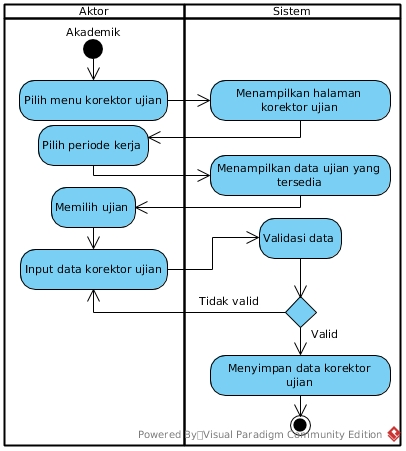
\includegraphics[width=11cm]{gambar/activity/input-data-korektor-ujian}
            		    \caption{\emph{Activity Diagram} Input Data Korektor Ujian}
            		    \label{activity_input_korektor}
            		\end{figure}
            		\emph{Activity Diagram} pada Gambar \ref{activity_input_korektor} menjelaskan bagaimana staf Akademik melakukan proses input data korektor ujian. Sebelum staf Akademik melakukan input data korektor ujian, staf Akademik perlu memilih periode kerja terlebih dahulu. Sistem akan menampilkan data ujian yang tersedia sesuai dengan periode kerja dan staff Akademik memilih ujian yang akan di input data korektornya. Kemudian sistem akan melakukan validasi sebelum menyimpan data korektor ujian tersebut.\newpage
            		\item Rekap Upah Pengawas Ujian
            		\begin{figure}[H]
            		    \centering            		    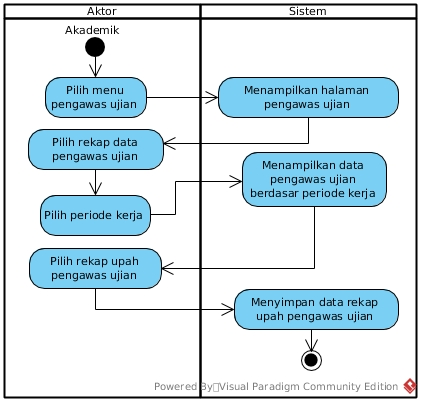
\includegraphics[width=11cm]{gambar/activity/rekap-upah-pengawas}
            		    \caption{\emph{Activity Diagram} Rekap Upah Pengawas Ujian}
            		    \label{activity_rekap_pengawas}
            		\end{figure}
            		\emph{Activity Diagram} pada Gambar \ref{activity_rekap_pengawas} menjelaskan bagaimana proses staf Akademik melakukan perekapan upah pengawas ujian. Pertama, pada halaman pengawas ujian staf Akademik memilih rekap data pengawas ujian. Kemudian staf Akademik memilih periode kerja dan sistem akan menampilkan data pengawas ujian berdasarkan periode kerja yang dipilih. Setelah itu staf Akademik dapat melakukan perekapan upah pengawas ujian selama satu periode yang dipilih.\newpage
            		\item Rekap Upah Korektor Ujian
            		\begin{figure}[H]
            		    \centering            		    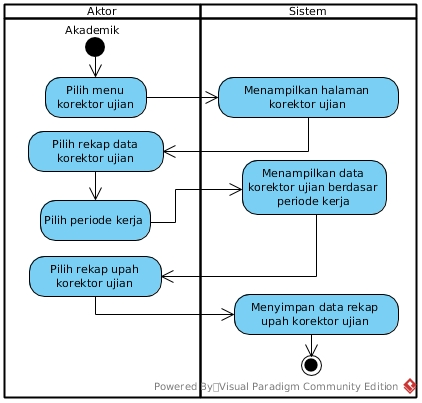
\includegraphics[width=11cm]{gambar/activity/rekap-upah-korektor}
            		    \caption{\emph{Activity Diagram} Rekap Upah Korektor Ujian}
            		    \label{activity_rekap_korektor}
            		\end{figure}
            		\emph{Activity Diagram} pada Gambar \ref{activity_rekap_korektor} menjelaskan bagaimana proses staf Akademik melakukan perekapan upah korektor ujian. Pada halaman korektor ujian staf Akademik memilih rekap data korektor ujian. Kemudian staf Akademik memilih periode kerja dan sistem akan menampilkan data korektor ujian berdasarkan periode kerja yang dipilih. Setelah itu staf Akademik dapat melakukan perekapan upah korektor ujian selama satu periode yang dipilih.\newpage
            		\item Lihat Data Pengawas Ujian
            	    \begin{figure}[H]
            		    \centering            		    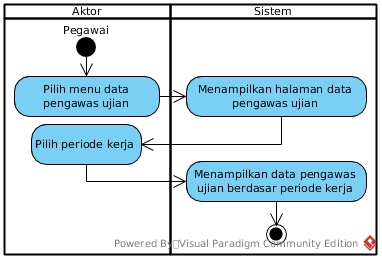
\includegraphics[width=11cm]{gambar/activity/lihat-data-pengawas-ujian}
            		    \caption{\emph{Activity Diagram} Lihat Data Pengawas Ujian}
            		    \label{activity_lihat_pengawas}
            		\end{figure}
            		\emph{Activity Diagram} pada Gambar \ref{activity_lihat_pengawas} menjelaskan bagaimana proses karyawan melihat data pengawas ujian. Karyawan memilih menu data pengawas ujian dan sistem menampilkan halaman pengawas ujian. Kemudian karyawan memilih periode kerja terlebih dahulu dan sistem akan menampilkan data pengawas ujian dari karyawan tersebut sesuai periode kerja yang dipilih.\newpage
            		\item Lihat Data Korektor Ujian
            	    \begin{figure}[H]
            		    \centering            		    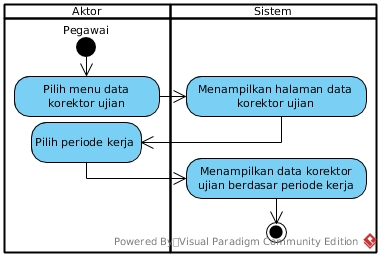
\includegraphics[width=11cm]{gambar/activity/lihat-data-korektor-ujian}
            		    \caption{\emph{Activity Diagram} Lihat Data Korektor Ujian}
            		    \label{activity_lihat_korektor}
            		\end{figure}
            		\emph{Activity Diagram} pada Gambar \ref{activity_lihat_korektor} menjelaskan bagaimana proses karyawan melihat data korektor ujian. Karyawan memilih menu data korektor ujian dan sistem menampilkan halaman korektor ujian. Kemudian karyawan memilih periode kerja terlebih dahulu dan sistem akan menampilkan data korektor ujian dari karyawan tersebut sesuai periode kerja yang dipilih.
            	\end{enumerate}
            	
            	\item \emph{Activity Diagram} Manajemen Laporan Kerja
            	
            	Dalam proses manajemen data laporan kerja karyawan terdapat beberapa \emph{activity} yang terdiri dari kategori input data dan kategori lihat data. Kategori input data meliputi input rencana kerja harian, input laporan kerja harian, input checklist bulanan dan input laporan kerja bulanan. Untuk kategori lihat data meliputi melihat seluruh laporan kerja baik harian maupun bulanan dan melihat detail kegiatan dari laporan kerja tersebut. Detail dari masing-masing \emph{activity} tersebut adalah sebagai berikut:\newpage
            		\begin{enumerate}[label=\alph*.]
            		    \itemsep0em
            		    \item Input Rencana Kerja Harian
            		    \begin{figure}[H]
                		    \centering                		    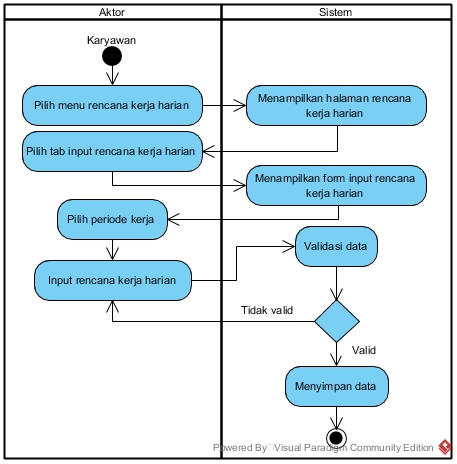
\includegraphics[width=11cm]{gambar/activity/input-rencana-kerja-harian}
                		    \caption{\emph{Activity Diagram} Input Rencana Kerja Harian}
                		    \label{activity_input_rkh}
                		\end{figure}
                		\emph{Activity Diagram} pada Gambar \ref{activity_input_rkh} menjelaskan bagaimana proses karyawan melakukan input data rencana kerja harian (RKH). Karyawan memilih menu RKH dan sistem akan menampilkan halaman data RKH. Kemudian karyawan memilih input RKH dan sistem akan menampilkan \emph{form} input RKH. Karyawan memilih periode kerja dan mengisi data RKH. Sistem akan melakukan validasi sebelum data RKH disimpan ke dalam \emph{database}.\newpage
            		    \item Input Laporan Kerja Harian
            		    \begin{figure}[H]
                		    \centering                		    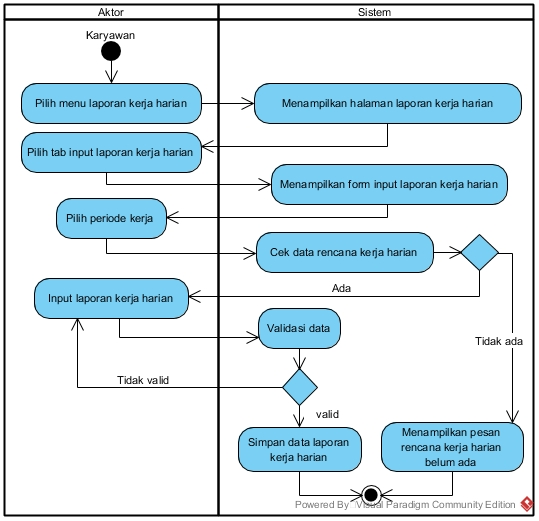
\includegraphics[width=11cm]{gambar/activity/input-laporan-kerja-harian}
                		    \caption{\emph{Activity Diagram} Input Laporan Kerja Harian}
                		    \label{activity_input_lh}
                		\end{figure}
                		\emph{Activity Diagram} pada Gambar \ref{activity_input_lh} menjelaskan bagaimana proses karyawan melakukan input data laporan kerja harian (LH). Karyawan memilih menu LH dan sistem akan menampilkan halaman data LH. Kemudian karyawan memilih input LH dan sistem akan menampilkan \emph{form} input LH. Karyawan memilih periode kerja dan sistem akan melakukan pengecekan data RKH sudah ada atau belum. Apabila RKH sudah ada, sistem akan menampilkan data RKH yang siap diisi LH-nya. Sistem akan melakukan validasi sebelum data LH disimpan ke dalam \emph{database}.\newpage
            		    \item Input Checklist Bulanan
            		    \begin{figure}[H]
                		    \centering                		    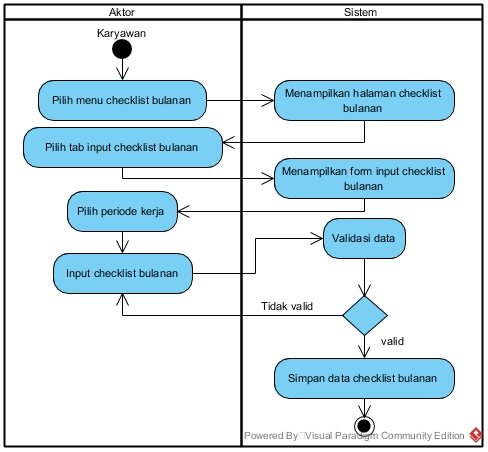
\includegraphics[width=11cm]{gambar/activity/input-checklist-bulanan}
                		    \caption{\emph{Activity Diagram} Input Checklist Bulanan}
                		    \label{activity_input_checklist}
                		\end{figure}
                		\emph{Activity Diagram} pada Gambar \ref{activity_input_checklist} menjelaskan bagaimana proses karyawan melakukan input data checklist bulanan (CB). Karyawan memilih menu CB dan sistem akan menampilkan halaman data CB. Kemudian karyawan memilih input CB dan sistem akan menampilkan \emph{form} input CB. Karyawan memilih periode kerja dan mengisi data CB. Sistem akan melakukan validasi sebelum data CB disimpan ke dalam \emph{database}.\newpage
            		    \item Input Laporan Kerja Bulanan
            		    \begin{figure}[H]
                		    \centering                		    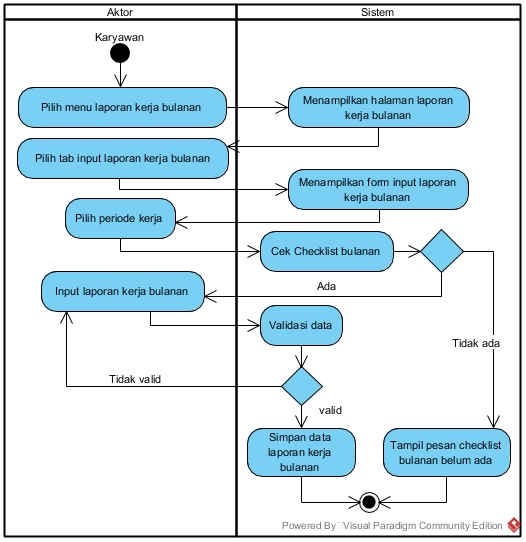
\includegraphics[width=11cm]{gambar/activity/input-laporan-kerja-bulanan}
                		    \caption{\emph{Activity Diagram} Input Laporan Kerja Bulanan}
                		    \label{activity_input_lb}
                		\end{figure}
                		\emph{Activity Diagram} pada Gambar \ref{activity_input_lb} menjelaskan bagaimana proses karyawan melakukan input data laporan kerja bulanan (LB). Karyawan memilih menu LB dan sistem akan menampilkan halaman data LB. Kemudian karyawan memilih input LB dan sistem akan menampilkan \emph{form} input LB. Karyawan memilih periode kerja dan sistem akan melakukan pengecekan data CB sudah ada atau belum. Apabila data CB sudah ada, sistem akan menampilkan data CB yang siap diisi LB-nya. Sistem akan melakukan validasi sebelum data LB disimpan ke dalam \emph{database}.\newpage
                		\item Lihat Laporan Kerja Karyawan
                		\begin{figure}[H]
            		        \centering            		    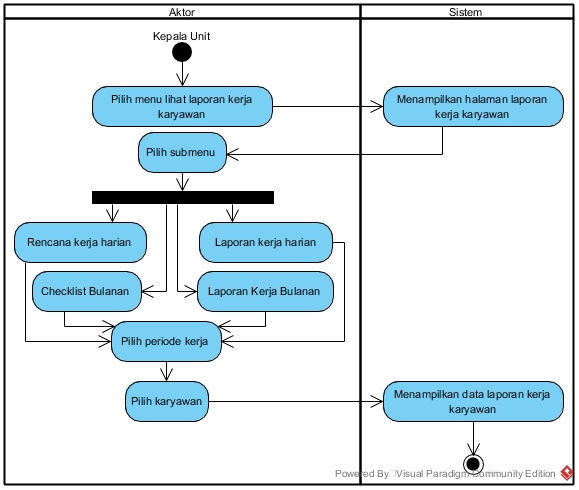
\includegraphics[width=13cm]{gambar/activity/lihat-laporan-kerja-pegawai}
            		        \caption{\emph{Activity Diagram} Lihat Laporan Kerja Karyawan}
            		        \label{activity_lihat_laporan_kerja}
            		    \end{figure}
            		    \emph{Activity Diagram} pada Gambar \ref{activity_lihat_laporan_kerja} menjelaskan bagaimana proses Kepala Unit melihat laporan kerja karyawan yang dibawahinya. Kepala Unit memilih menu laporan kerja karyawan dan sistem menampilkan halaman laporan kerja karyawan. Kemudian memilih antara laporan kerja harian atau laporan kerja bulanan. Setelah itu Kepala Unit memilih periode kerja dan nama karyawan yang dibawahinya. Sistem akan menampilkan data laporan kerja karyawan sesuai periode dan nama karyawan yang dipilih.\newpage
            		\end{enumerate}
            	
            	\item \emph{Activity Diagram} Manajemen Penilaian Kinerja Karyawan
            	
            	Dalam proses manajemen penilaian kinerja karyawan terdapat beberapa \emph{activity} yang meliputi input penilaian kinerja karyawan dan lihat data penilaian kinerja karyawan. Detail dari masing-masing \emph{activity} tersebut adalah sebagai berikut:
            	\begin{enumerate}[label=\alph*.]
            	    \itemsep0em
            	    \item Input Penilaian Kinerja Karyawan
            	    \begin{figure}[H]
            		    \centering
            		    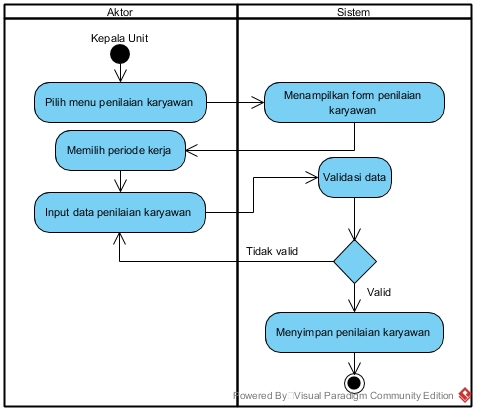
\includegraphics[width=11cm]{gambar/activity/input-penilaian-pegawai}
            		    \caption{\emph{Activity Diagram} Input Penilaian Kinerja Karyawan}
            		    \label{activity_input_penilaian}
            		\end{figure}
            		\emph{Activity Diagram} pada Gambar \ref{activity_input_penilaian} menjelaskan bagaimana Kepala Unit memberikan penilaian kinerja kepada karyawan yang dibawahinya. Kepala Unit memilih menu penilaian kinerja dan sistem akan menampilkan form penilaian karyawan. Sebelum input data penilaian, Kepala Unit harus memilih periode kerja terlebih dahulu. Sistem akan melakukan validasi sebelum data penilaian kinerja disimpan ke dalam sistem.
            	    \item Lihat Data Penilaian Kinerja Karyawan
            	    \begin{figure}[H]
            		    \centering
            		    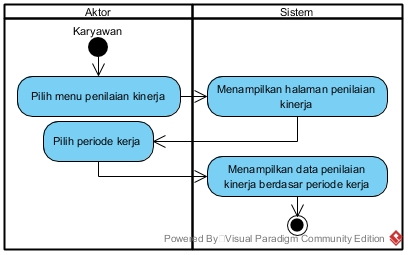
\includegraphics[width=9cm]{gambar/activity/lihat-data-penilaian-kinerja}
            		    \caption{\emph{Activity Diagram} Lihat Data Penilaian Kinerja}
            		    \label{activity_lihat_penilaian}
            		\end{figure}
            		\emph{Activity Diagram} pada Gambar \ref{activity_lihat_penilaian} menjelaskan proses bagaimana karyawan melihat data penilaian kinerja. Karyawan memilih memilih periode kerja dan sistem akan menampilkan data sesuai periode kerja yang dipilih.
            	\end{enumerate}
            	    
            	\item \emph{Activity Diagram} Input Insentif Operasional
            	    \begin{figure}[H]
            		    \centering
            		    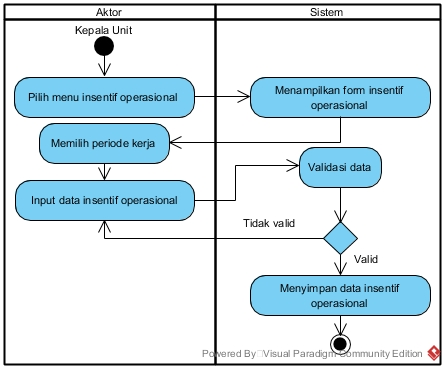
\includegraphics[width=10cm]{gambar/activity/input-insentif-operasional}
            		    \caption{\emph{Activity Diagram} Input Insentif Operasional}
            		    \label{activity_input_insentif}
            		\end{figure}
            		\emph{Activity Diagram} pada Gambar \ref{activity_input_insentif} menjelaskan bagaimana Kepala Unit memberikan insentif operasional kepada karyawan yang dibawahinya. Kepala Unit memilih menu insentif operasional dan sistem akan menampilkan form input insentif operasional. Sebelum input data insentif operasional, Kepala Unit harus memilih periode kerja terlebih dahulu. Sistem akan melakukan validasi sebelum data insentif operasional tersebut disimpan ke dalam sistem. 
            	 \item \emph{Activity Diagram} Manajemen Gaji Karyawan
            	 
            	 Proses manajemen gaji karyawan ini terdiri dari beberapa \emph{activity} yang meliputi \emph{generate} slip gaji, lihat data slip gaji, cetak slip gaji, dan lihat laporan penggajian. Detail dari masing-masing \emph{activity} tersebut adalah sebagai berikut:
                \begin{enumerate}[label=\alph*.]
            	     \itemsep0em
            	     \item \emph{Generate} Slip Gaji
            	     \begin{figure}[H]
            		    \centering
            		    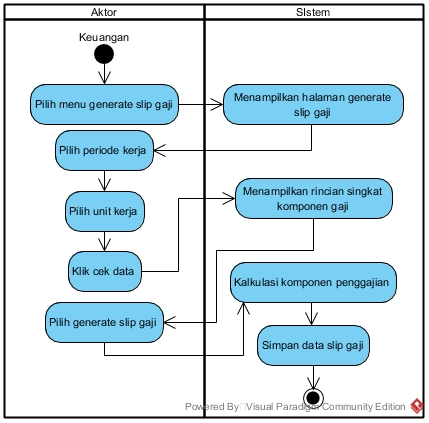
\includegraphics[width=10cm]{gambar/activity/generate-slip-gaji}
            		    \caption{\emph{Activity Diagram Generate} Slip Gaji}
            		    \label{activity_generate_slip}
                    \end{figure}
                    \emph{Activity Diagram} pada Gambar \ref{activity_generate_slip} menjelaskan bagaimana staf Keuangan melakukan \emph{generate} slip gaji karyawan. Di dalam halaman \emph{generate} slip gaji, staf Keuangan memilih periode kerja dan unit kerja, kemudian sistem akan menampilkan rincian komponen gaji karyawan. Setelah itu Keuangan dapat memilih \emph{generate} slip gaji, kemudian sistem akan menyimpan hasil kalkulasi dan data slip gaji tersebut.
            	    \item Cetak Slip Gaji
            	    \begin{figure}[H]
            		    \centering
            		    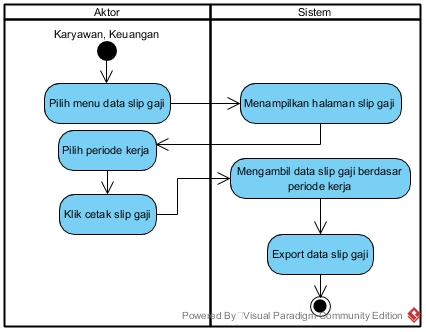
\includegraphics[width=10cm]{gambar/activity/cetak-slip-gaji}
            		    \caption{\emph{Activity Diagram} Cetak Slip Gaji}
            		    \label{activity_cetak_slip}
            		\end{figure}
            		\emph{Activity Diagram} pada Gambar \ref{activity_cetak_slip} menjelaskan bagaimana karyawan melakukan proses cetak slip gaji. Pada halaman cetak slip gaji, karyawan memilih periode kerja terlebih dahulu dan klik cetak slip gaji. Kemudian sistem akan mengambil data slip gaji berdasarkan periode yang dipilih dan melakukan \emph{export} data slip gaji tersebut.
            		\newpage
            		\item Lihat Laporan Penggajian
            		\begin{figure}[H]
            		    \centering
            		    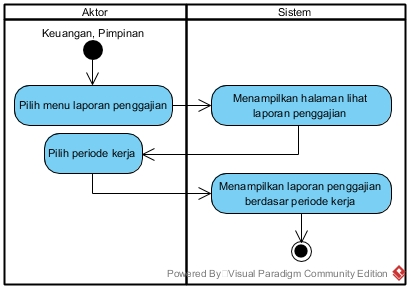
\includegraphics[width=10cm]{gambar/activity/lihat-laporan-penggajian}
            		    \caption{\emph{Activity Diagram} Lihat Laporan Penggajian}
            		    \label{activity_laporan_penggajian}
            		\end{figure}
            		\emph{Activity Diagram} pada Gambar \ref{activity_laporan_penggajian} menjelaskan bagaimana Keuangan dan Pimpinan melihat laporan penggajian karyawan. Pada halaman lihat laporan penggajian, kedua aktor tersebut memilih periode kerja terlebih dahulu. Setelah itu sistem akan mengambil dan menampilkan data laporan penggajian karyawan berdasarkan periode kerja yang dipilih.
                \end{enumerate}
			\end{enumerate}
			
			
			\subsubsection{\emph{Sequence Diagram}}
			Perancangan \emph{sequence} bertujuan untuk menjelaskan secara detail urutan proses yang dilakukan di dalam sistem untuk mencapai tujuan dari \emph{Use Case} yang telah digambarkan sebelumnya. Berikut \emph{Sequence Diagram} yang menggambarkan masing-masing \emph{sequence}:
			\newpage
			\begin{enumerate}
			    \itemsep0em
			    \item \emph{Sequence Diagram} Login
			        \begin{figure}[H]
            		    \centering
            		    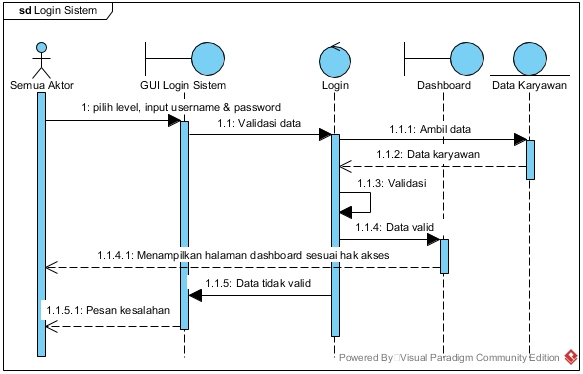
\includegraphics[width=13cm]{gambar/sequence/seq-login}
            		    \caption{\emph{Sequence Diagram} Login}
            		    \label{sequence_login}
            		\end{figure}
            		\emph{Sequence Diagram} pada Gambar \ref{sequence_login} menjelaskan bagaimana urutan proses semua Aktor \emph{Login} ke dalam sistem. Pertama Aktor harus memilih level atau hak aksesnya, kemudian memasukkan \emph{username} dan \emph{password}. Sistem akan melakukan validasi data tersebut berdasarkan data karyawan. Apabila level yang dipilih sesuai dengan \emph{username} dan \emph{password} maka sistem akan menampilkan halaman \emph{Dashboard} sesuai levelnya. Sedangkan apabila data yang dimasukan salah, sistem akan menampilkan pesan kesalahan. \newpage
			    \item \emph{Sequence Diagram} Manajemen Data Karyawan
			        \begin{figure}[H]
            		    \centering
            		    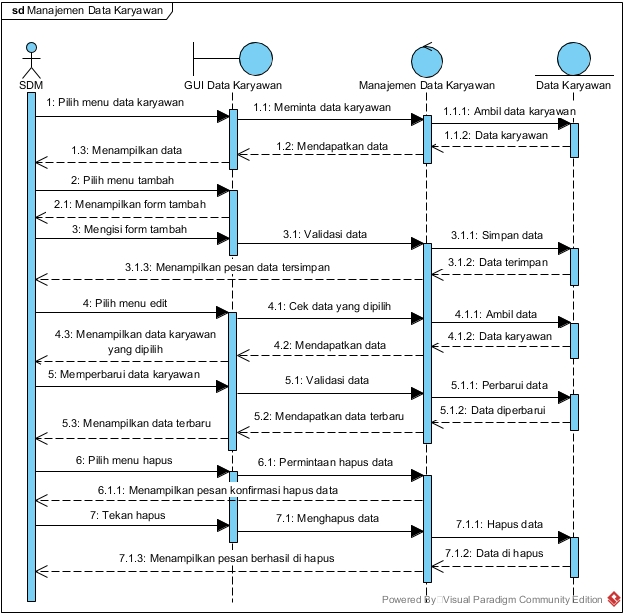
\includegraphics[width=14cm]{gambar/sequence/manajemen-pegawai}
            		    \caption{\emph{Sequence Diagram} Manajemen Data Karyawan}
            		    \label{sequence_manajemen_pegawai}
            		\end{figure}
            		\emph{Sequence Diagram} pada Gambar \ref{sequence_manajemen_pegawai} menjelaskan bagaimana urutan proses SDM melakukan manajemen data karyawan, meliputi tambah data, ubah data dan hapus data. Proses dimulai ketika SDM memilih menu data karyawan dan sistem akan meminta data karyawan untuk ditampilkan kepada SDM. Ketika memilih tambah karyawan, sistem akan menampilkan form yang akan diisi oleh SDM. Sebelum disimpan ke dalam \emph{database} karyawan, sistem akan melakukan validasi terlebih dahulu. Kemudian sistem akan menampilkan pesan apabila data berhasil disimpan ke dalam \emph{database}.
            		
            		Ketika memilih edit data karyawan, sistem akan menampilkan detail data karyawan yang dipilih dan SDM dapat mengubah data tersebut. Seperti tindakan tambah karyawan, sebelum mengubah data karyawan sistem juga akan melakukan validasi.
            		
            		Ketika SDM ingin menghapus data karyawan, sistem akan menampilkan pesan konfirmasi apakah data benar-benar ingin dihapus sebelum menekan tombol hapus.
            	\item \emph{Sequence Diagram} Manajemen Data Unit Kerja
			        \begin{figure}[H]
            		    \centering
            		    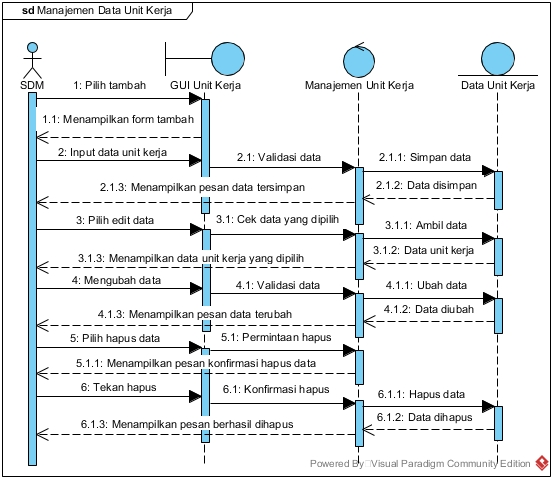
\includegraphics[width=13cm]{gambar/sequence/manajemen-unit-kerja}
            		    \caption{\emph{Sequence Diagram} Manajemen Data Unit Kerja}
            		    \label{sequence_manajemen_unitkerja}
            		\end{figure}
            		\emph{Sequence Diagram} pada Gambar \ref{sequence_manajemen_unitkerja} menjelaskan bagaimana urutan proses SDM melakukan manajemen data unit kerja, meliputi tambah data, ubah data dan hapus data. Ketika memilih tambah data, sistem akan menampilkan form dan SDM mengisi data unit kerja. Sistem akan melakukan validasi data sebelum disimpan dan akan menampilkan pesan apabila data berhasil disimpan ke dalam \emph{database} Unit Kerja.
            		
            		Pada pilihan edit data, sistem akan mengambil data unit kerja yang dipilih dan menampilkannya kepada SDM. Kemudian SDM dapat mengubah data tersebut dan menyimpannya. Sebelum disimpan sistem akan melakukan validasi terlebih dahulu. Sistem akan menampilkan pesan bahwa data berhasil diperbarui. Proses hapus data unit kerja sama dengan proses hapus data karyawan. Sistem akan menampilkan pesan konfirmasi terlebih dahulu.
            	\item \emph{Sequence Diagram} Manajemen Data Jabatan
			        \begin{figure}[H]
            		    \centering
            		    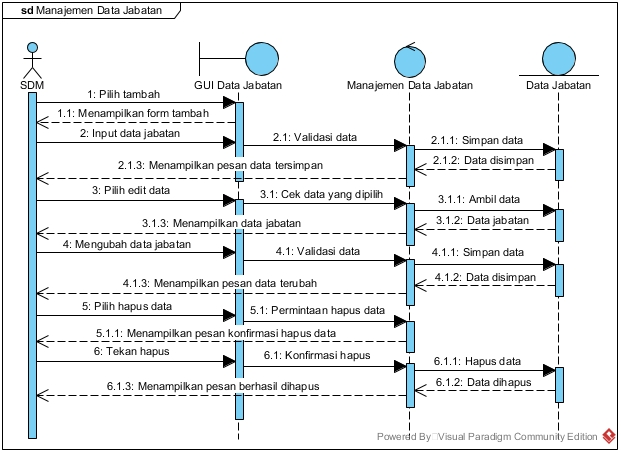
\includegraphics[width=13cm]{gambar/sequence/manajemen-jabatan}
            		    \caption{\emph{Sequence Diagram} Manajemen Data Jabatan}
            		    \label{sequence_manajemen_jabatan}
            		\end{figure}
            		\emph{Sequence Diagram} pada Gambar \ref{sequence_manajemen_jabatan} menjelaskan bagaimana urutan proses SDM melakukan manajemen data jabatan. Ketika memilih tambah data, sistem akan menampilkan form dan SDM mengisi data jabatan. Sistem akan melakukan validasi data sebelum disimpan dan akan menampilkan pesan apabila data berhasil disimpan ke dalam \emph{database} Jabatan.
            		
            		Pada pilihan edit data, sistem akan mengambil data jabatan yang dipilih dan menampilkannya kepada SDM. Kemudian SDM dapat mengubah data tersebut dan menyimpannya. Sebelum disimpan sistem akan melakukan validasi terlebih dahulu. Sistem akan menampilkan pesan bahwa data berhasil diperbarui. Proses hapus data jabatan sama dengan proses hapus data karyawan. Sistem akan menampilkan pesan konfirmasi terlebih dahulu.
            	\item \emph{Sequence Diagram} Manajemen Status Kepegawaian
			        \begin{figure}[H]
            		    \centering            		    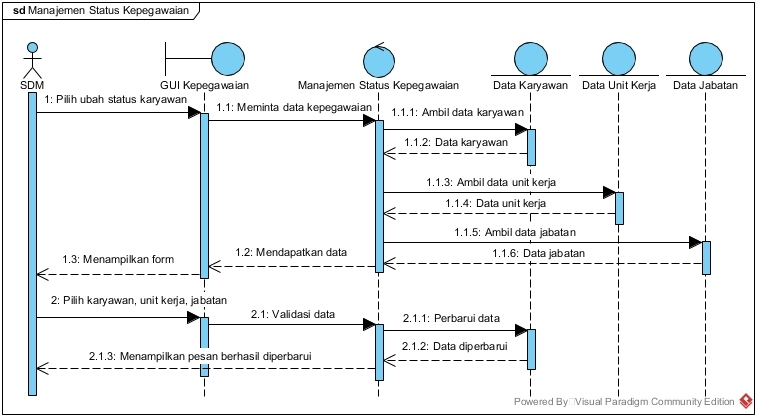
\includegraphics[width=14cm]{gambar/sequence/manajemen-status-kepegawaian}
            		    \caption{\emph{Sequence Diagram} Manajemen Status Kepegawaian}
            		    \label{sequence_manajemen_kepegawaian}
            		\end{figure}
            		\emph{Sequence Diagram} pada Gambar \ref{sequence_manajemen_kepegawaian} menjelaskan bagaimana urutan proses SDM melakukan manajemen status kepegawaian karyawan. Maksud dari status kepegawaian adalah unit kerja dan jabatan dari karyawan. Langkah pertama SDM memilih tindakan ubah status karyawan. Kemudian sistem akan mengambil data karyawan, data unit kerja dan data jabatan dari dalam \emph{database} untuk ditampilkan kepada SDM. Kemudian SDM memilih karyawan, data unit kerja dan data jabatan yang menjadi tujuan. Sistem akan melakukan validasi data sebelum data disimpan dan menampilkan pesan apabila data berhasil diperbarui ke dalam \emph{database}.
            	\item \emph{Sequence Diagram} Input Data Periode Kerja
			        \begin{figure}[H]
            		    \centering
            		    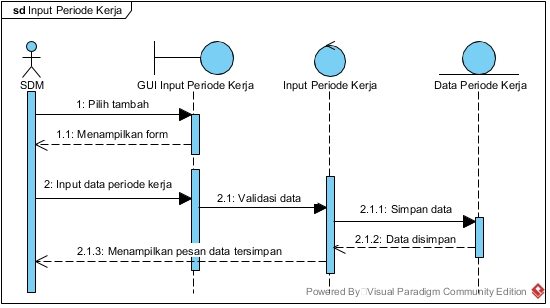
\includegraphics[width=13cm]{gambar/sequence/input-periode-kerja}
            		    \caption{\emph{Sequence Diagram} Input Data Periode Kerja}
            		    \label{sequence_input_periode}
            		\end{figure}
            		\emph{Sequence Diagram} pada Gambar \ref{sequence_input_periode} menjelaskan bagaimana urutan proses SDM melakukan \emph{input} data periode kerja. SDM memilih tambah data, dan sistem akan menampilkan \emph{form input} data. Kemudian SDM akan mengisi data periode kerja pada \emph{form} tersebut. Sistem akan melakukan validasi data terlebih dahulu sebelum disimpan ke dalam \emph{database} Periode Kerja. Sistem akan menampilkan pesan data tersimpan apabila data berhasil disimpan. \newpage
            	\item \emph{Sequence Diagram} Manajemen Data Rapat
            	
            	Dalam urutan proses manajemen data rapat terdapat terdapat beberapa \emph{sequence diagram} meliputi input data rapat, rekap upah rapat dan lihat data rapat. Detail dari masing-masing \emph{sequence} tersebut adalah sebagai berikut:
            	\begin{enumerate}[label=\alph*.]
            	    \itemsep0em
            	    \item Input Data Rapat
            	    \begin{figure}[H]
            		    \centering
            		    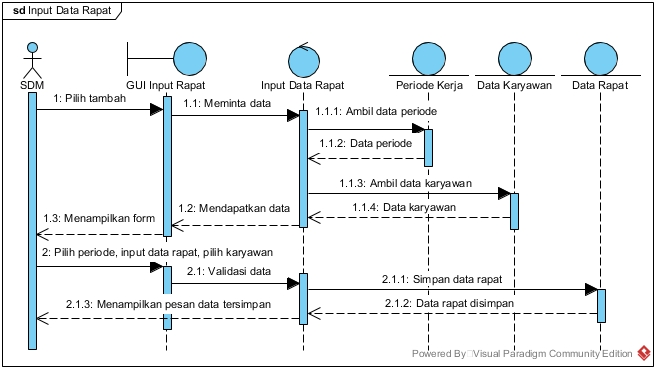
\includegraphics[width=14cm]{gambar/sequence/input-data-rapat}
            		    \caption{\emph{Sequence Diagram} Input Data Rapat}
            		    \label{sequence_input_rapat}
            		\end{figure}
            		\emph{Sequence Diagram} pada Gambar \ref{sequence_input_rapat} menjelaskan bagaimana urutan proses SDM melakukan \emph{input} data rapat karyawan. Langkah pertama adalah SDM memilih tambah data rapat, dan sistem akan mengambil data periode kerja dan data karyawan dari \emph{database} untuk ditampilkan pada \emph{form} tambah data rapat. Pada form tersebut SDM dapat memilih periode kerja dimana rapat tersebut dilaksanakan, memilih karyawan selaku peserta rapat dan data rapat lainnya. Sebelum data disimpan ke dalam \emph{database}, sistem akan melakukan validasi data terlebih dahulu. Kemudian sistem akan menampilkan pesan data tersimpan apabila data berhasil disimpan ke dalam \emph{database} Data Rapat. \newpage
            	    \item Rekap Upah Rapat
            	    \begin{figure}[H]
            		    \centering
            		    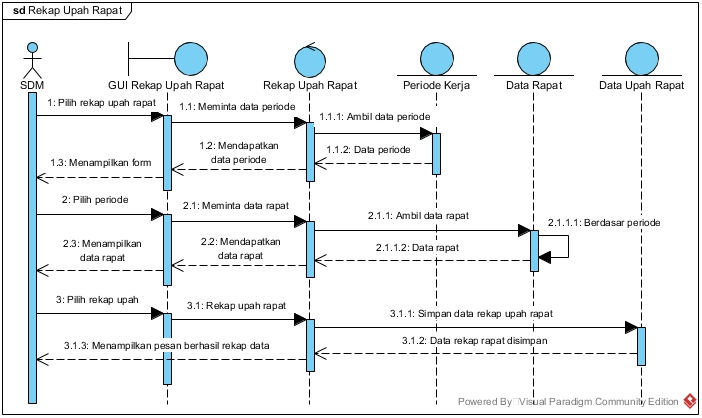
\includegraphics[width=13cm]{gambar/sequence/rekap-upah-rapat}
            		    \caption{\emph{Sequence Diagram} Rekap Upah Rapat}
            		    \label{sequence_upah_rapat}
            		\end{figure}
            		\emph{Sequence Diagram} pada Gambar \ref{sequence_upah_rapat} menjelaskan bagaimana urutan proses SDM melakukan perekapan upah rapat karyawan. Pertama SDM memilih rekap upah rapat dan sistem akan mengambil data periode kerja untuk ditampilkan dalam \emph{form}. SDM memilih periode kerja, kemudian sistem akan menampilkan data rapat karyawan selama periode yang dipilih. Setelah itu SDM dapat memilih rekap upah rapat karyawan sesuai data yang telah ditampilkan. Sistem akan melakukan perekapan upah rapat dan menyimpannya ke dalam \emph{database} data upah rapat. \newpage
            	    \item Lihat Data Rapat
            	    \begin{figure}[H]
            		    \centering
            		    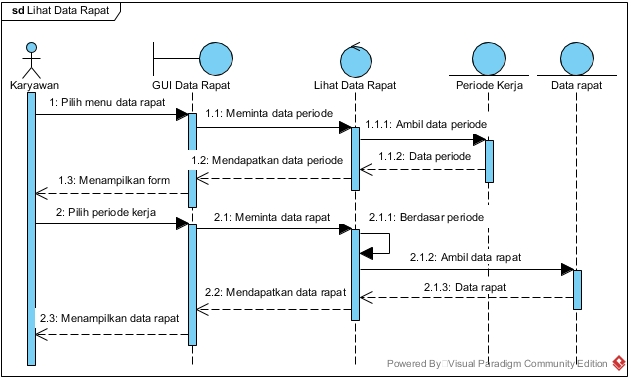
\includegraphics[width=13cm]{gambar/sequence/lihat-data-rapat}
            		    \caption{\emph{Sequence Diagram} Lihat Data Rapat}
            		    \label{sequence_lihat_rapat}
            		\end{figure}
            		\emph{Sequence Diagram} pada Gambar \ref{sequence_lihat_rapat} menjelaskan bagaimana urutan proses Karyawan melihat data rapat yang dihadiri oleh karyawan tersebut. Karyawan memilih lihat data rapat dan sistem akan mengambil data periode kerja dari dalam \emph{database} untuk ditampilkan pada \emph{form}. Setelah itu karyawan dapat memilih periode kerja sebagai parameter. Kemudian sistem mengambil data rapat berdasarkan periode kerja yang telah dipilih sebelumnya.
            	\end{enumerate}
			        
            	\item \emph{Sequence Diagram} Manajemen Data Lembur
            	
            	Dalam urutan proses manajemen data lembur terdapat terdapat beberapa \emph{sequence diagram} meliputi input data lembur, rekap upah lembur dan lihat data lembur. Detail dari masing-masing \emph{sequence} tersebut adalah sebagai berikut: \newpage
            	\begin{enumerate}[label=\alph*.]
            	    \itemsep0em
            	    \item Input Data Lembur
            	    \begin{figure}[H]
            		    \centering            		    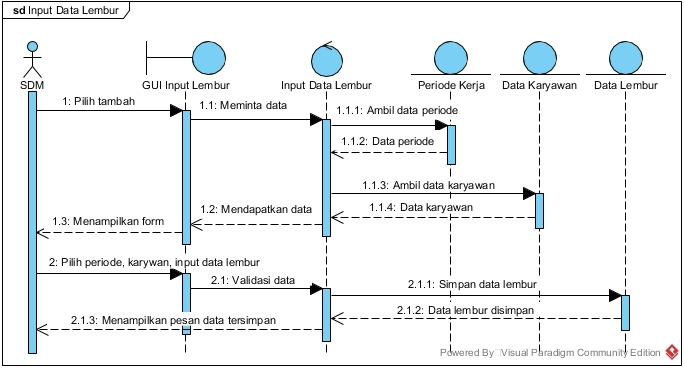
\includegraphics[width=14cm]{gambar/sequence/input-data-lembur}
            		    \caption{\emph{Sequence Diagram} Input Data Lembur}
            		    \label{sequence_input_lembur}
            		\end{figure}
            		\emph{Sequence Diagram} pada Gambar \ref{sequence_input_lembur} menjelaskan bagaimana urutan proses SDM melakukan \emph{input} data lembur karyawan. Langkah pertama adalah SDM memilih tambah data lembur, dan sistem akan mengambil data periode kerja dan data karyawan dari \emph{database} untuk ditampilkan pada \emph{form}. Pada form tersebut SDM dapat memilih periode kerja dimana lembur karyawan tersebut dilaksanakan, memilih karyawan yang lembur dan data lembur lainnya. Sebelum data disimpan ke dalam \emph{database}, sistem akan melakukan validasi data terlebih dahulu. Kemudian sistem akan menampilkan pesan data tersimpan apabila data berhasil disimpan ke dalam \emph{database} Data Lembur. \newpage
            	    \item Rekap Upah Lembur
            	    
            	    \emph{Sequence Diagram} yang menjelaskan urutan proses rekap upah lembur karyawan tidak jauh berbeda dengan urutan proses rekap upah rapat. Yang berbeda yaitu entitas yang digunakan adalah data lembur karyawan.
            	    \item Lihat Data Lembur
            	    \begin{figure}[H]
            		    \centering            		    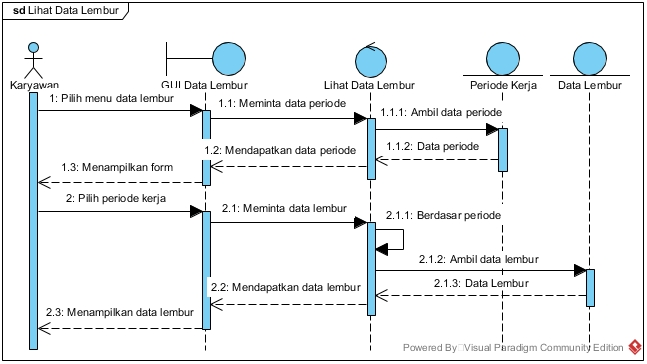
\includegraphics[width=13cm]{gambar/sequence/lihat-data-lembur}
            		    \caption{\emph{Sequence Diagram} Lihat Data Lembur}
            		    \label{sequence_lihat_lembur}
            		\end{figure}
            		\emph{Sequence Diagram} pada Gambar \ref{sequence_lihat_lembur} menjelaskan bagaimana urutan proses karyawan melihat data lembur. Langkah pertama karyawan memilih lihat data lembur dan sistem akan mengambil data periode kerja dari dalam \emph{database} untuk ditampilkan pada \emph{form}. Kemudian karyawan dapat memilih periode kerja sebagai parameter inputan. Setelah itu sistem mengambil data lembur karyawan berdasarkan periode kerja yang telah dipilih sebelumnya. \newpage
            	\end{enumerate}
			        
            	\item \emph{Sequence Diagram} Manajemen Data Absensi
            	
            	Dalam urutan proses manajemen data absensi karyawan terdapat terdapat beberapa \emph{sequence diagram} meliputi \emph{upload} data absensi, ubah data absensi dan lihat rekap absensi. Detail dari masing-masing \emph{sequence} tersebut adalah sebagai berikut:
            	\begin{enumerate}[label=\alph*.]
            	    \itemsep0em
            	    \item \emph{Upload} Data Absensi
            	    \begin{figure}[H]
            		    \centering            		    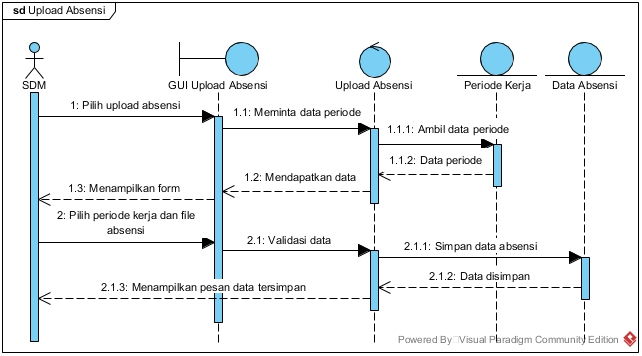
\includegraphics[width=13cm]{gambar/sequence/upload-data-absensi}
            		    \caption{\emph{Sequence Diagram} Upload Absensi}
            		    \label{sequence_upload_absensi}
            		\end{figure}
            		\emph{Sequence Diagram} pada Gambar \ref{sequence_upload_absensi} menjelaskan bagaimana urutan proses SDM melakukan \emph{upload} data absensi ke dalam sistem. Langkah pertama adalah SDM memilih tindakan \emph{upload} absensi, dan sistem akan mengambil data periode kerja dari \emph{database} untuk ditampilkan pada \emph{form upload} absensi. Pada \emph{form} tersebut SDM memilih periode kerja dari absensi dan memilih \emph{file} absensi. Sistem akan melakukan validasi data terlebih dahulu sebelum disimpan ke dalam \emph{database}. Kemudian sistem akan menampilkan pesan data tersimpan apabila data berhasil disimpan ke dalam \emph{database} Data Absensi. \newpage
            	    \item Lihat Rekap Absensi
            	    \begin{figure}[H]
            		    \centering
            		    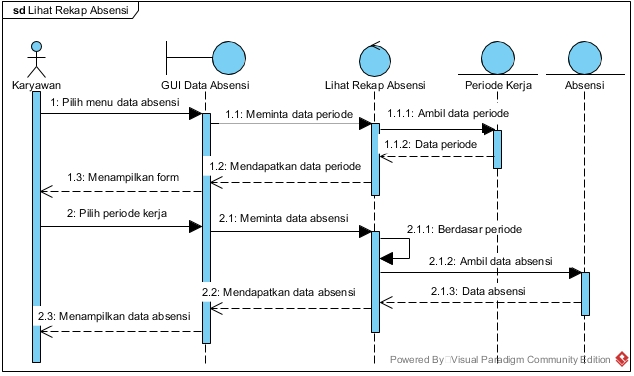
\includegraphics[width=13cm]{gambar/sequence/lihat-rekap-absensi}
            		    \caption{\emph{Sequence Diagram} Lihat Rekap Absensi}
            		    \label{sequence_lihat_absensi}
            		\end{figure}
            		\emph{Sequence Diagram} pada Gambar \ref{sequence_lihat_absensi} menjelaskan bagaimana urutan proses karyawan melihat data rekap absensi. Pertama karyawan memilih lihat data absensi dan sistem akan mengambil data periode kerja dari dalam \emph{database} untuk ditampilkan pada \emph{form}. Setelah itu karyawan dapat memilih periode kerja sebagai parameter. Kemudian sistem mengambil data absensi karyawan tersebut berdasarkan periode kerja yang telah dipilih sebelumnya. \newpage
            	\end{enumerate}
			        
            	\item \emph{Sequence Diagram} Manajemen Data Ujian
            	
            	Dalam urutan proses manajemen data ujian terdapat terdapat beberapa \emph{sequence} meliputi input data ujian, pengawas dan korektor ujian, rekap upah pengawas dan korektor ujian, serta lihat data pengawas dan kotektor ujian. Detail dari masing-masing \emph{sequence} tersebut adalah sebagai berikut:
            	\begin{enumerate}[label=\alph*.]
            	    \itemsep0em
            	    \item Input Data Ujian
            	    \begin{figure}[H]
            		    \centering            		    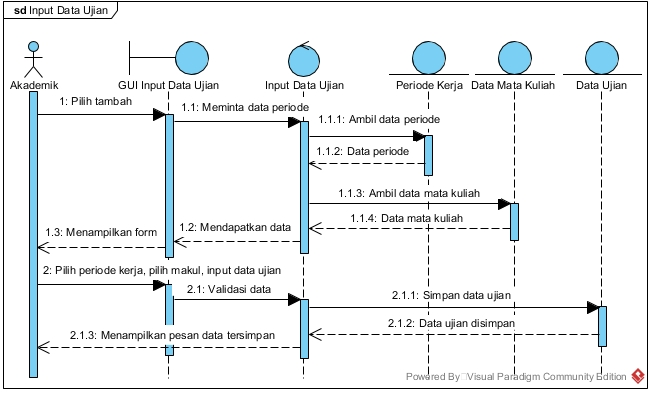
\includegraphics[width=13cm]{gambar/sequence/input-data-ujian}
            		    \caption{\emph{Sequence Diagram} Input Data Ujian}
            		    \label{sequence_input_ujian}
            		\end{figure}
            		\emph{Sequence Diagram} pada Gambar \ref{sequence_input_ujian} menjelaskan bagaimana urutan proses Akademik melakukan \emph{input} data ujian. Akademik memilih tambah data ujian, kemudian sistem akan mengambil data periode kerja dan data mata kuliah dari dalam \emph{database} untuk ditampilkan pada \emph{form} tambah data. Pada \emph{form} tersebut Akademik memilih periode kerja, mata kuliah ujian dan data ujian lainnya. Kemudian sistem akan melakukan validasi data sebelum disimpan ke dalam \emph{database}. Terakhir sistem akan menampilkan pesan data tersimpan apabila data berhasil disimpan ke dalam \emph{database} Data Ujian. \newpage
            	    \item Input Data Pengawas Ujian
            	    \begin{figure}[H]
            		    \centering
            		    \includegraphics[width=14cm]{gambar/sequence/input-data-pengawas}
            		    \caption{\emph{Sequence Diagram} Input Data Pengawas Ujian}
            		    \label{sequence_input_pengawas}
            		\end{figure}
            		\emph{Sequence Diagram} pada Gambar \ref{sequence_input_pengawas} menjelaskan bagaimana urutan proses Akademik mengisi data pengawas ujian. Pertama Akademik memilih tambah data pengawas dan sistem akan mengambil data periode kerja dari dalam \emph{database} untuk ditampilkan pada \emph{form}. Pada \emph{form} tersebut Akademik akan memilih periode kerja, kemudian sistem akan mengambil data ujian sesuai periode kerja yang dipilih dan ditampilkan dalam \emph{form}. Setelah itu Akademik memilih ujian dan karyawan yang menjadi pengawas ujian tersebut. Sistem akan melakukan validasi sebelum data disimpan. Terakhir sistem akan menampilkan pesan data tersimpan apabila data berhasil disimpan ke dalam \emph{database} Pengawas Ujian. \newpage
            	    \item Input Data Korektor Ujian
            	    \begin{figure}[H]
            		    \centering
            		    \includegraphics[width=14cm]{gambar/sequence/input-data-korektor}
            		    \caption{\emph{Sequence Diagram} Input Data Korektor Ujian}
            		    \label{sequence_input_korektor}
            		\end{figure}
            		\emph{Sequence Diagram} pada Gambar \ref{sequence_input_korektor} menjelaskan bagaimana urutan proses Akademik mengisi data korektor ujian. Pertama Akademik memilih tambah data korektor dan sistem akan mengambil data periode kerja dari dalam \emph{database} untuk ditampilkan pada \emph{form}. Pada \emph{form} tersebut Akademik akan memilih periode kerja, kemudian sistem akan mengambil data ujian sesuai periode kerja yang dipilih dan ditampilkan dalam \emph{form}. Setelah itu Akademik memilih ujian dan karyawan yang menjadi korektor ujian tersebut. Sistem akan melakukan validasi sebelum data disimpan. Terakhir sistem akan menampilkan pesan data tersimpan apabila data berhasil disimpan ke dalam \emph{database} Korektor Ujian. \newpage
            	    \item Lihat Data Pengawas Ujian
            	    \begin{figure}[H]
            		    \centering
            		    \includegraphics[width=13cm]{gambar/sequence/lihat-data-pengawas}
            		    \caption{\emph{Sequence Diagram} Lihat Data Pengawas Ujian}
            		    \label{sequence_lihat_pengawas}
            		\end{figure}
            		\emph{Sequence Diagram} pada Gambar \ref{sequence_lihat_pengawas} menjelaskan bagaimana urutan proses karyawan melihat data pengawas ujian. Langkah pertama karyawan memilih lihat data pengawas ujian dan sistem akan mengambil data periode kerja dari dalam \emph{database} untuk ditampilkan pada \emph{form}. Setelah itu karyawan dapat memilih periode kerja sebagai parameter. Kemudian sistem mengambil data pengawas ujian yang dilakukan oleh karyawan berdasarkan periode kerja yang telah dipilih sebelumnya.
            	    \item Lihat Data Korektor Ujian
            	    
            	    \emph{Sequence Diagram} untuk lihat data korektor ujian tidak jauh berbeda dengan lihat data pengawas ujian, hanya saja entitas yang digunakan adalah data korektor ujian.
            	    \item Rekap Upah Pengawas dan Korektor Ujian
            	    
            	    \emph{Sequence Diagram} untuk urutan proses rekap upah pengawas dan korektor ujian juga tidak jauh berbeda dengan urutan proses rekap upah rapat ataupun lembur.
            	\end{enumerate}
            	    
            	\item \emph{Sequence Diagram} Manajemen Laporan Kerja Karyawan
            	
            	Dalam urutan proses manajamen data laporan kerja karyawan terdapat beberapa \emph{sequence} meliputi input rencana kerja dan laporan harian, input checklist dan laporan bulanan, serta lihat data laporan kerja. Penjelasan dari masing-masing \emph{sequence} adalah sebagai berikut:
            	\begin{enumerate}[label=\alph*.]
            	    \itemsep0em
            	    \item Input Rencana Kerja Harian
            	    \begin{figure}[H]
            		    \centering            		    \includegraphics[width=14cm]{gambar/sequence/input-propeka-rkh}
            		    \caption{\emph{Sequence Diagram} Input Rencana Kerja Harian}
            		    \label{sequence_input_propeka_rkh}
            		\end{figure}
            		\emph{Sequence Diagram} pada Gambar \ref{sequence_input_propeka_rkh} menjelaskan bagaimana urutan proses karyawan melakukan input data rencana kerja harian (RKH). Pada \emph{form} tambah data RKH, karyawan memilih periode kerja dan tanggal. Sistem kemudian akan melakukan pengecekan apakah data RKH untuk periode dan tanggal yang dipilih sudah ada atau belum. Apabila sudah ada maka sistem akan menampilkan pesan bahwa RKH untuk periode dan tanggal yang dipilih sudah diisi. Sedangkan apabila data belum ada, karyawan dapat melakukan pengisian data RKH berupa rencana kegiatan-kegiatan selama satu hari.
            	    \item Input Laporan Kerja Harian
            	    \begin{figure}[H]
            		    \centering            		    \includegraphics[width=14cm]{gambar/sequence/input-propeka-lh}
            		    \caption{\emph{Sequence Diagram} Input Laporan Kerja Harian}
            		    \label{sequence_input_propeka_lh}
            		\end{figure}
            		\emph{Sequence Diagram} pada Gambar \ref{sequence_input_propeka_lh} menjelaskan bagaimana urutan proses karyawan melakukan input data laporan kerja harian (LH). Karyawan terlebih dahulu memilih periode kerja dan tanggal. Kemudian sistem akan mengecek ketersediaan data RKH dalam \emph{database}. Apabila data RKH tidak ada, maka sistem akan menampilkan pesan bahwa RKH untuk tanggal yang dipilih belum dibuat. Sedangkan apabila data RKH sudah ada, sistem akan menampilkan kegiatan-kegiatan RKH beserta \emph{form} untuk mengisi data LH.
            	    \item Input Checklist Bulanan
            	    \begin{figure}[H]
            		    \centering            		    \includegraphics[width=14cm]{gambar/sequence/input-propeka-cb}
            		    \caption{\emph{Sequence Diagram} Input Checklist Bulanan}
            		    \label{sequence_input_propeka_cb}
            		\end{figure}
            		\emph{Sequence Diagram} pada Gambar \ref{sequence_input_propeka_cb} menjelaskan bagaimana urutan proses karyawan melakukan input data rencana kerja bulanan atau biasa disebut checklist bulanan (CB). Pada \emph{form} tambah data CB, karyawan harus memilih periode kerja terlebih dahulu sebagai parameter. Sistem kemudian akan melakukan pengecekan apakah data CB untuk periode yang dipilih sudah ada atau belum. Apabila sudah ada maka sistem akan menampilkan pesan bahwa CB untuk periode yang dipilih sudah diisi. Sedangkan apabila data belum ada, karyawan dapat melakukan pengisian data CB berupa rencana kegiatan-kegiatan selama satu periode kerja.
            	    \item Input Laporan Kerja Bulanan
            	    \begin{figure}[H]
            		    \centering            		    \includegraphics[width=14cm]{gambar/sequence/input-propeka-lb}
            		    \caption{\emph{Sequence Diagram} Input Laporan Kerja Bulanan}
            		    \label{sequence_input_propeka_lb}
            		\end{figure}
            		\emph{Sequence Diagram} pada Gambar \ref{sequence_input_propeka_lb} menjelaskan bagaimana urutan proses karyawan melakukan input data laporan kerja bulanan (LB). Karyawan terlebih dahulu memilih periode kerja sebagai parameter. Kemudian sistem akan mengecek ketersediaan data checklist bulanan (CB) dalam \emph{database}. Apabila data CB tidak ada, maka sistem akan menampilkan pesan bahwa CB untuk periode kerja yang dipilih belum dibuat. Sedangkan apabila data CB sudah ada, sistem akan menampilkan kegiatan-kegiatan CB beserta \emph{form} untuk mengisi data LB.
            	\end{enumerate}
            	\newpage
            	\item \emph{Sequence Diagram} Manajemen Penilaian Kinerja Karyawan
            	
            	Proses manajemen penilaian kinerja karyawan ini memiliki beberapa \emph{sequence} yang meliputi input penilaian kinerja dan lihat data penilaian kinerja. Detail dari masing-masing \emph{sequence} tersebut adalah sebagai berikut:
            	\begin{enumerate}[label=\alph*.]
            	    \itemsep0em
            	    \item Input Penilaian Kinerja
            	    \begin{figure}[H]
            		    \centering
            		    \includegraphics[width=14cm]{gambar/sequence/input-penilaian-kinerja}
            		    \caption{\emph{Sequence Diagram} Input Penilaian Kinerja Karyawan}
            		    \label{sequence_input_penilaian}
            		\end{figure}
            		\emph{Sequence Diagram} pada Gambar \ref{sequence_input_penilaian} menjelaskan bagaimana urutan proses Kepala Unit mengisi data penilaian kinerja karyawan yang dibawahinya. Pada halaman penilaian kinerja, Kepala Unit memilih input penilaian dan sistem akan mengambil data periode kerja dan data karyawan untuk ditampilkan ke dalam \emph{form} penilaian. Setelah itu Kepala Unit memilih periode kerja dan mengisi penilaian kinerja karyawan. Kemudian sistem akan melakukan validasi data tersebut sebelum disimpan ke dalam \emph{database}. Sistem akan menampilkan pesan data tersimpan apabila data berhasil disimpan. \newpage
            	    \item Lihat Data Penilaian Kinerja
            	    \begin{figure}[H]
            		    \centering
            		    \includegraphics[width=13cm]{gambar/sequence/lihat-data-penilaian}
            		    \caption{\emph{Sequence Diagram} Lihat Data Penilaian Kinerja}
            		    \label{sequence_lihat_penilaian}
            		\end{figure}
            		\emph{Sequence Diagram} pada Gambar \ref{sequence_lihat_penilaian} menjelaskan bagaimana urutan proses karyawan melihat data penilaian kinerja. Pertama karyawan memilih lihat data penilaian dan sistem akan mengambil data periode kerja dari dalam \emph{database} untuk ditampilkan pada \emph{form}. Setelah itu karyawan dapat memilih periode kerja sebagai parameter. Kemudian sistem mengambil data penilaian kinerja karyawan tersebut berdasarkan periode kerja yang telah dipilih sebelumnya. \newpage
            	\end{enumerate}
			        
            	\item \emph{Sequence Diagram} Input Insentif Operasional
            	    \begin{figure}[H]
            		    \centering
            		    \includegraphics[width=14cm]{gambar/sequence/input-insentif-operasional}
            		    \caption{\emph{Sequence Diagram} Input Insentif Operasional}
            		    \label{sequence_input_insentif}
            		\end{figure}
            		\emph{Sequence Diagram} pada Gambar \ref{sequence_input_insentif} menjelaskan bagaimana urutan proses Kepala Unit mengisi data insentif operasional karyawan yang dibawahinya. Pada halaman insentif operasional, Kepala Unit memilih tambah insentif operasional dan sistem akan mengambil data periode kerja dan data karyawan untuk ditampilkan ke dalam \emph{form} input insentif operasional. Setelah itu Kepala Unit memilih periode kerja dan mengisi data insentif operasional karyawan. Kemudian sistem akan melakukan validasi data tersebut sebelum disimpan ke dalam \emph{database}. Sistem akan menampilkan pesan data tersimpan apabila data berhasil disimpan. \newpage
			        
            	\item \emph{Sequence Diagram Generate} Slip Gaji
			        \begin{figure}[H]
            		    \centering            		    \includegraphics[width=14cm]{gambar/sequence/generate-slip-gaji}
            		    \caption{\emph{Sequence Diagram Generate} Slip Gaji}
            		    \label{sequence_generate_slip}
            		\end{figure}
            		\emph{Sequence Diagram} pada Gambar \ref{sequence_generate_slip} menjelaskan bagaimana urutan proses staf Keuangan melakukan \emph{generate} slip gaji karyawan. Pertama sistem akan mengambil data periode kerja dan data unit kerja untuk ditampilkan dalam \emph{form}. Kemudian staf Keuangan memilih periode kerja dan unit kerja sebagai parameter. Sistem akan mengambil data upah karyawan berdasarkan periode kerja dan unit kerja yang dipilih, dan melakukan kalkulasi upah karyawan tersebut. Lalu sistem akan menampilkannya kepada staf Keuangan. Setelah itu staf Keuangan memilih \emph{generate} slip gaji dan sistem akan melakukan proses \emph{generate} slip dan menyimpannya ke dalam \emph{database}.
            		\newpage
            	\item \emph{Sequence Diagram} Cetak Slip Gaji
			        \begin{figure}[H]
            		    \centering            		    \includegraphics[width=12cm]{gambar/sequence/cetak-slip-gaji}
            		    \caption{\emph{Sequence Diagram} Cetak Slip Gaji}
            		    \label{sequence_cetak_slip}
            		\end{figure}
            		\emph{Sequence Diagram} pada Gambar \ref{sequence_cetak_slip} menjelaskan bagaimana urutan proses karyawan melakukan cetak slip gaji. Karyawan memilih periode kerja dan sistem akan mengambil data slip gaji karyawan berdasarkan periode yang dipilih. Kemudian sistem menampilkan data slip gaji tersebut kepada karyawan. Setelah itu karyawan memilih cetak slip gaji, dan sistem akan melakukan \emph{export} data slip gaji tersebut.
			\end{enumerate}
			
			\subsubsection{\emph{Entity Relationship Diagram}}
			Peneliti selanjutnya membuat ERD dengan tujuan untuk menjelaskan keterkaitan antara data satu dengan yang lainnya. Berdasarkan ERD pada Gambar \ref{erd_penggajian}, nantinya akan diketahui secara garis besar tabel apa saja yang dibutuhkan oleh sistem yang dikembangkan.
			\newpage
			\begin{figure}[H]
			    \centering
			    \includegraphics[width=14cm]{gambar/entity/ERD-versi3}
			    \caption{ERD Sistem Informasi Penggajian Karyawan}
			    \label{erd_penggajian}
			\end{figure}

		\subsection{Perancangan Basis Data}
		Perancangan basis data merupakan rancangan struktur tabel yang nantinya akan menjadi basis data dari sistem yang dikembangkan.
		
		    \subsubsection{Hasil Rancangan Basis Data}
		    Berikut merupakan hasil dari perancangan basis data pada sistem yang dikembangkan:
		    \begin{enumerate}
		        \itemsep0em
			    \item Tabel Bidang Kerja (\texttt{master\_bidang})
		        
		        Tabel Bidang Kerja berfungsi untuk menyimpan data bidang kerja. Selanjutnya tabel tersebut diberi nama \texttt{master\_bidang}. Detail dari tabel tersebut dapat dilihat pada Tabel \ref{tabel_bidang}.
		        \begin{spacing}{1.0}
		        \begin{longtable}{|>{\centering}p{1.5em}|p{3cm}|p{3cm}|p{3cm}|p{2cm}|}
			        \caption{Tabel Bidang Kerja (\texttt{master\_bidang})} \label{tabel_bidang} \\
                    \hline \textbf{No.} & \textbf{Colomn} & \textbf{Type} & \textbf{Constraint} & \textbf{Extra}  \\ \hline 
                    \endfirsthead
                    \multicolumn{5}{c}%
                    {{\bfseries \tablename\ \thetable{}: }Tabel Bidang Kerja (\texttt{master\_bidang}) (lanjutan)} \\
                    \hline \textbf{No.} & \textbf{Colomn} & \textbf{Type} & \textbf{Constraint} & \textbf{Extra}  \\ \hline
                    \endhead
                    \hline
                    \hline \hline
                    \endlastfoot
                    
                    1. & kode\_bidang & character varying(10) & PRIMARY KEY, NOT NULL & \\ \hline
                    2. & nama\_bidang & character varying(30) & NOT NULL & \\ \hline
                    3. & keterangan & character varying(50) & & \\ \hline
			    \end{longtable}
			    \end{spacing}
			    \vspace{4mm}
		        \item Tabel Unit Kerja (\texttt{master\_unit\_kerja})
		        
		        Tabel Unit Kerja berfungsi untuk menyimpan data unit kerja. Selanjutnya tabel tersebut diberi nama \texttt{master\_unit\_kerja}. Detail dari tabel tersebut dapat dilihat pada Tabel \ref{tabel_unit_kerja}.
		        \begin{spacing}{1.0}
		        \begin{longtable}{|>{\centering}p{1.5em}|p{3cm}|p{3cm}|p{3cm}|p{2cm}|}
			        \caption{Tabel Unit Kerja (\texttt{master\_unit\_kerja})} \label{tabel_unit_kerja} \\
                    \hline \textbf{No.} & \textbf{Colomn} & \textbf{Type} & \textbf{Constraint} & \textbf{Extra}  \\ \hline 
                    \endfirsthead
                    \multicolumn{5}{c}%
                    {{\bfseries \tablename\ \thetable{}: }Tabel Unit Kerja (\texttt{master\_unit\_kerja}) (lanjutan)} \\
                    \hline \textbf{No.} & \textbf{Colomn} & \textbf{Type} & \textbf{Constraint} & \textbf{Extra}  \\ \hline
                    \endhead
                    \hline
                    \endfoot
                    \hline \hline
                    \endlastfoot
                    
                    1. & kode\_unit & character varying(20) & PRIMARY KEY, NOT NULL & \\ \hline
                    2. & kode\_bidang & character varying(10) & NOT NULL & \\ \hline
                    3. & nama\_unit & character varying(50) & & \\ \hline
                    4. & keterangan & character varying(50) & & \\ \hline
			    \end{longtable}
			    \end{spacing}
			    \vspace{4mm}
		        \item Tabel Jabatan (\texttt{master\_jabatan})
		        
		        Tabel Jabatan berfungsi untuk menyimpan data master jabatan yang ada di Universitas Proklamasi 45 Yogyakarta. Selanjutnya tabel tersebut diberi nama \texttt{master\_jabatan}. Detail dari tabel master jabatan dapat dilihat pada Tabel \ref{tabel_jabatan}.
		        \begin{spacing}{1.0}
		        \begin{longtable}{|>{\centering}p{1.5em}|p{3cm}|p{3cm}|p{3cm}|p{2cm}|}
			        \caption{Tabel Jabatan (\texttt{master\_jabatan})} \label{tabel_jabatan} \\
                    \hline \textbf{No.} & \textbf{Colomn} & \textbf{Type} & \textbf{Constraint} & \textbf{Extra}  \\ \hline 
                    \endfirsthead
                    \multicolumn{5}{c}%
                    {{\bfseries \tablename\ \thetable{}: }Tabel Jabatan (\texttt{master\_jabatan}) (lanjutan)} \\
                    \hline \textbf{No.} & \textbf{Colomn} & \textbf{Type} & \textbf{Constraint} & \textbf{Extra}  \\ \hline
                    \endhead
                    \hline
                    \endfoot
                    \hline \hline
                    \endlastfoot
                    
                    1. & kode\_jabatan & character varying(20) & PRIMARY KEY, NOT NULL & \\ \hline
                    2. & nama\_jabatan & character varying(50) & NOT NULL & \\ \hline
                    3. & tunjangan\_jabatan & integer & NOT NULL & default: 0 \\ \hline
                    4. & keterangan & character varying(50) & & \\ \hline
                    5. & under\_of\_jabatan & character varying(20) & NOT NULL & \\ \hline
                    6. & max\_satu & enum (ya,tidak) &  & default: ya \\ \hline
                    7. & tersedia & enum (ya,tidak) & & default: ya \\ \hline
                    
			    \end{longtable}
			    \end{spacing}
			    \vspace{4mm}
			    \newpage
		        \item Tabel Periode Kerja (\texttt{master\_periode})
		        
		        Tabel periode kerja berfungsi untuk menyimpan data master periode kerja. Selanjutnya tabel tersebut diberi nama \texttt{master\_periode}. Detail dari tabel periode kerja dapat dilihat pada Tabel \ref{tabel_periode}.
		        \begin{spacing}{1.0}
		        \begin{longtable}{|>{\centering}p{1.5em}|p{3cm}|p{3cm}|p{3cm}|p{2cm}|}
			        \caption{Tabel Periode Kerja (\texttt{master\_periode})} \label{tabel_periode} \\
                    \hline \textbf{No.} & \textbf{Colomn} & \textbf{Type} & \textbf{Constraint} & \textbf{Extra}  \\ \hline 
                    \endfirsthead
                    \multicolumn{5}{c}%
                    {{\bfseries \tablename\ \thetable{}: }Tabel Periode Kerja (\texttt{master\_periode}) (lanjutan)} \\
                    \hline \textbf{No.} & \textbf{Colomn} & \textbf{Type} & \textbf{Constraint} & \textbf{Extra}  \\ \hline
                    \endhead
                    \hline
                    \endfoot
                    \hline \hline
                    \endlastfoot
                    
                    1. & id\_periode & integer & PRIMARY KEY, NOT NULL & Auto Increment \\ \hline
                    2. & tahun & year(4) & NOT NULL & \\ \hline
                    3. & bulan & character varying(15) & NOT NULL & \\ \hline
                    4. & mulai & date & NOT NULL & \\ \hline
                    5. & akhir & date & NOT NULL & \\ \hline
                    6. & hari\_aktif & integer & NOT NULL & \\ \hline
                    7. & pembagi & float & NOT NULL & \\ \hline
                    8. & aktif & enum (ya,tidak) & & default: tidak \\ \hline
			    \end{longtable}
			    \end{spacing}
			    \vspace{4mm}
			    \item Tabel Jam Kerja (\texttt{master\_jam\_kerja})
			    
			    Tabel jam kerja berfungsi untuk menyimpan data master jam kerja karyawan. Selanjutnya tabel tersebut diberi nama \texttt{master\_jam\_kerja}. Detail dari tabel jam kerja dapat dilihat pada Tabel \ref{tabel_jam_kerja}.
			    \begin{spacing}{1.0}
		        \begin{longtable}{|>{\centering}p{1.5em}|p{3.5cm}|p{2.5cm}|p{3cm}|p{2cm}|}
			        \caption{Tabel Jam Kerja (\texttt{master\_jam\_kerja})} \label{tabel_jam_kerja} \\
                    \hline \textbf{No.} & \textbf{Colomn} & \textbf{Type} & \textbf{Constraint} & \textbf{Extra}  \\ \hline 
                    \endfirsthead
                    \multicolumn{5}{c}%
                    {{\bfseries \tablename\ \thetable{}: }Tabel Jam Kerja (\texttt{master\_jam\_kerja}) (lanjutan)} \\
                    \hline \textbf{No.} & \textbf{Colomn} & \textbf{Type} & \textbf{Constraint} & \textbf{Extra}  \\ \hline
                    \endhead
                    \hline
                    \endfoot
                    \hline \hline
                    \endlastfoot
                    
                    1. & kode\_jam\_kerja & character varying(20) & PRIMARY KEY, NOT NULL & \\ \hline
                    2. & nama\_jam\_kerja & character varying(30) & NOT NULL & \\ \hline
                    3. & jumlah\_jam & integer & NOT NULL & \\ \hline
                    4. & jam\_datang & time & NOT NULL & \\ \hline
                    5. & jam\_pulang & time & NOT NULL & \\ \hline
                    6. & jam\_istirahat & time & NOT NULL & \\ \hline
                    7. & toleransi & time & NOT NULL & \\ \hline
                    8. & jam\_datang\_sabtu & time & NOT NULL & \\ \hline
                    9. & jam\_pulang\_sabtu & time & NOT NULL & \\ \hline
                    10. & jam\_istirahat\_sabtu & time & NOT NULL & \\ \hline
                    11. & toleransi\_sabtu & time & NOT NULL & \\ \hline
			    \end{longtable}
			    \end{spacing}
			    \vspace{4mm}
		        \item Tabel Nominal (\texttt{master\_nominal})
		        
		        Tabel nominal berfungsi untuk menyimpan data master besaran nominal upah dan juga potongan yang termasuk komponen penggajian. Selanjutnya tabel tersebut diberi nama \texttt{master\_nominal}. Detail dari tabel nominal dapat dilihat pada Tabel \ref{tabel_nominal}.
		        \begin{spacing}{1.0}
		        \begin{longtable}{|>{\centering}p{1.5em}|p{3cm}|p{3cm}|p{3cm}|p{2cm}|}
			        \caption{Tabel Nominal (\texttt{master\_nominal})} \label{tabel_nominal} \\
                    \hline \textbf{No.} & \textbf{Colomn} & \textbf{Type} & \textbf{Constraint} & \textbf{Extra}  \\ \hline 
                    \endfirsthead
                    \multicolumn{5}{c}%
                    {{\bfseries \tablename\ \thetable{}: }Tabel Nominal (\texttt{master\_nominal}) (lanjutan)} \\
                    \hline \textbf{No.} & \textbf{Colomn} & \textbf{Type} & \textbf{Constraint} & \textbf{Extra}  \\ \hline
                    \endhead
                    \hline
                    \endfoot
                    \hline \hline
                    \endlastfoot
                    
                    1. & id\_nominal & integer & PRIMARY KEY, NOT NULL & Auto Increment \\ \hline
                    2. & tpd & integer & NOT NULL & \\ \hline
                    3. & lembur & integer & NOT NULL & \\ \hline
                    4. & uang\_makan & integer & NOT NULL & \\ \hline
                    5. & rapat & integer & NOT NULL & \\ \hline
                    6. & transport\_reguler & integer & NOT NULL & \\ \hline
                    7. & transport\_malam & integer & NOT NULL & \\ \hline
                    8. & sks & integer & NOT NULL & \\ \hline
                    9. & tunjangan\_bpjs & integer & NOT NULL & \\ \hline
                    10. & potongan\_bpjs & integer & NOT NULL & \\ \hline
                    11. & potongan\_koperasi & integer & NOT NULL & \\ \hline
                    12. & hal\_khusus & integer & NOT NULL & \\ \hline
                    13. & korektor\_ujian & integer & NOT NULL & \\ \hline
                    14. & pengawas\_reguler & integer & NOT NULL & \\ \hline
                    15. & pengawas\_malam & integer & NOT NULL & \\ \hline
                    16. & aktif & enum (ya,tidak) & & default: tidak \\ \hline
			    \end{longtable}
			    \end{spacing}
			    \vspace{4mm}
		        \item Tabel Program Studi (\texttt{master\_program\_studi})
		        
		        Tabel program studi berfungsi menyimpan data nama-nama program studi yang ada. Selanjutnya tabel tersebut diberi nama \texttt{master\_prodi}. Detail tabel program studi dapat dilihat pada Tabel \ref{tabel_prodi}.
		        \begin{spacing}{1.0}
		        \begin{longtable}{|>{\centering}p{1.5em}|p{3cm}|p{3cm}|p{3cm}|p{2cm}|}
			        \caption{Tabel Program Studi (\texttt{master\_prodi})} \label{tabel_prodi} \\
                    \hline \textbf{No.} & \textbf{Colomn} & \textbf{Type} & \textbf{Constraint} & \textbf{Extra}  \\ \hline 
                    \endfirsthead
                    \multicolumn{5}{c}%
                    {{\bfseries \tablename\ \thetable{}: }Tabel Program Studi (\texttt{master\_prodi}) (lanjutan)} \\
                    \hline \textbf{No.} & \textbf{Colomn} & \textbf{Type} & \textbf{Constraint} & \textbf{Extra}  \\ \hline
                    \endhead
                    \hline
                    \endfoot
                    \hline \hline
                    \endlastfoot
                    
                    1. & kode\_prodi & character varying(10) & PRIMARY KEY, NOT NULL & \\ \hline
                    2. & nama\_prodi & character varying(50) & NOT NULL & \\ \hline
                    3. & kode\_fakultas & character varying(20) & NOT NULL & \\ \hline
                    4. & keterangan & character varying(50) & & \\ \hline
			    \end{longtable}
			    \end{spacing}
			    \vspace{4mm}
		        \item Tabel Mata Kuliah (\texttt{master\_matakuliah})
		        
		        Tabel mata kuliah berfungsi menyimpan data nama-nama mata kuliah yang ada. Selanjutnya tabel tersebut diberi nama \texttt{master\_matakuliah}. Detail tabel mata kuliah dapat dilihat pada Tabel \ref{tabel_makul}.
		        \begin{spacing}{1.0}
		        \begin{longtable}{|>{\centering}p{1.5em}|p{3cm}|p{3cm}|p{3cm}|p{2cm}|}
			        \caption{Tabel Mata Kuliah (\texttt{master\_matakuliah})} \label{tabel_makul} \\
                    \hline \textbf{No.} & \textbf{Colomn} & \textbf{Type} & \textbf{Constraint} & \textbf{Extra}  \\ \hline 
                    \endfirsthead
                    \multicolumn{5}{c}%
                    {{\bfseries \tablename\ \thetable{}: }Tabel Mata Kuliah (\texttt{master\_matakuliah}) (lanjutan)} \\
                    \hline \textbf{No.} & \textbf{Colomn} & \textbf{Type} & \textbf{Constraint} & \textbf{Extra}  \\ \hline
                    \endhead
                    \hline
                    \endfoot
                    \hline \hline
                    \endlastfoot
                    
                    1. & kode\_matakuliah & character varying(10) & PRIMARY KEY, NOT NULL & \\ \hline
                    2. & nama\_matakuliah & character varying(50) & NOT NULL & \\ \hline
                    3. & sks\_matakuliah & integer & NOT NULL & \\ \hline
                    4. & smt\_matakuliah & integer & NOT NULL & \\ \hline
                    5. & kode\_prodi & character varying(10) & FOREIGN KEY, NOT NULL & \\ \hline
			    \end{longtable}
			    \end{spacing}
			    \vspace{4mm}
			    \item Tabel Karyawan (\texttt{data\_pegawai})
		        
		        Tabel Karyawan berfungsi untuk menyimpan data karyawan. Selanjutnya tabel tersebut diberi nama \texttt{data\_pegawai}. Detail dari tabel karyawan dapat dilihat pada Tabel \ref{tabel_karyawan}.
		        \begin{spacing}{1.0}
		        \begin{longtable}{|>{\centering}p{1.5em}|p{3cm}|p{3cm}|p{3cm}|p{2cm}|}
			        \caption{Tabel Karyawan (\texttt{data\_karyawan})} \label{tabel_karyawan} \\
                    \hline \textbf{No.} & \textbf{Colomn} & \textbf{Type} & \textbf{Constraint} & \textbf{Extra}  \\ \hline 
                    \endfirsthead
                    \multicolumn{5}{c}%
                    {{\bfseries \tablename\ \thetable{}: }Tabel Karyawan (\texttt{data\_karyawan}) (lanjutan)} \\
                    \hline \textbf{No.} & \textbf{Colomn} & \textbf{Type} & \textbf{Constraint} & \textbf{Extra}  \\ \hline
                    \endhead
                    \hline
                    \endfoot
                    \hline \hline
                    \endlastfoot
                    
                    1. & nip & character varying(30) & PRIMARY KEY, NOT NULL & \\ \hline
                    2. & nama & character varying(50) & NOT NULL & \\ \hline
                    3. & email & character varying(30) & & \\ \hline
                    4. & status\_karyawan & character varying(10) & & \\ \hline
                    5. & kode\_jam\_kerja & character varying(10) & FOREIGN KEY, NOT NULL & \\ \hline
                    6. & kode\_unit & character varying(20) & FOREIGN KEY, NOT NULL & \\ \hline
                    7. & kode\_jabatan & character varying(20) & FOREIGN KEY, NOT NULL & \\ \hline
                    8. & gaji\_pokok & integer & NOT NULL & \\ \hline
                    9. & tgppw & integer & NOT NULL & \\ \hline
                    10. & bpjs\_aktif & enum (ya,tidak) & & default: tidak \\ \hline
                    11. & koperasi\_aktif & enum (ya,tidak) & & default: tidak \\ \hline
                    12. & username & character varying(20) & NOT NULL & \\ \hline
                    13. & password & character varying(64) & NOT NULL & \\ \hline
			    \end{longtable}
			    \end{spacing}
			    \vspace{4mm}
		        \item Tabel Data Absensi (\texttt{absensi\_data})
		        
		        Tabel data absensi berfungsi menyimpan data absensi harian masing-masing karyawan. Selanjutnya tabel absensi tersebut diberi nama \texttt{absensi\_data}. Detail dari tabel absensi dapat dilihat pada Tabel \ref{tabel_absensi}.
		        \begin{spacing}{1.0}
		        \begin{longtable}{|>{\centering}p{1.5em}|p{3cm}|p{3cm}|p{3cm}|p{2cm}|}
			        \caption{Tabel Data Absensi (\texttt{absensi\_data})} \label{tabel_absensi} \\
                    \hline \textbf{No.} & \textbf{Colomn} & \textbf{Type} & \textbf{Constraint} & \textbf{Extra}  \\ \hline 
                    \endfirsthead
                    \multicolumn{5}{c}%
                    {{\bfseries \tablename\ \thetable{}: }Tabel Data Absensi (\texttt{absensi\_data}) (lanjutan)} \\
                    \hline \textbf{No.} & \textbf{Colomn} & \textbf{Type} & \textbf{Constraint} & \textbf{Extra}  \\ \hline
                    \endhead
                    \hline
                    \endfoot
                    \hline \hline
                    \endlastfoot
                    
                    1. & id\_absensi & integer & PRIMARY KEY, NOT NULL & Auto Increment \\ \hline
                    2. & id\_periode & integer & FOREIGN KEY, NOT NULL & \\ \hline
                    3. & tanggal & date & NOT NULL & \\ \hline
                    4. & hari & character varying(10) & NOT NULL & \\ \hline
                    5. & nip & character varying(30) & FOREIGN KEY, NOT NULL & \\ \hline
                    6. & datang & time & NOT NULL & \\ \hline
                    7. & pulang & time & NOT NULL & \\ \hline
                    8. & lama\_kerja & time & NOT NULL & \\ \hline
                    9. & telat & enum (0,1) & NOT NULL & \\ \hline
                    10. & keterangan & character varying(30) & & \\ \hline
			    \end{longtable}
			    \end{spacing}
			    \vspace{4mm}
		        \item Tabel Rekap Absensi (\texttt{absensi\_rekap})
		        
		        Tabel rekap absensi berfungsi untuk menyimpan hasil rekap data absensi harian masing-masing karyawan dalam satu periode kerja. Selanjutnya tabel tersebut diberi nama \texttt{absensi\_rekap}. Detail dari tabel rekap absensi dapat dilihat pada Tabel \ref{tabel_absensi_rekap}.
		        \begin{spacing}{1.0}
		        \begin{longtable}{|>{\centering}p{1.5em}|p{3cm}|p{2.5cm}|p{3cm}|p{2.5cm}|}
			        \caption{Tabel Rekap Absensi (\texttt{absensi\_rekap})} \label{tabel_absensi_rekap} \\
                    \hline \textbf{No.} & \textbf{Colomn} & \textbf{Type} & \textbf{Constraint} & \textbf{Extra}  \\ \hline 
                    \endfirsthead
                    \multicolumn{5}{c}%
                    {{\bfseries \tablename\ \thetable{}: }Tabel Rekap Absensi (\texttt{absensi\_rekap}) (lanjutan)} \\
                    \hline \textbf{No.} & \textbf{Colomn} & \textbf{Type} & \textbf{Constraint} & \textbf{Extra}  \\ \hline
                    \endhead
                    \hline
                    \endfoot
                    \hline \hline
                    \endlastfoot
                    
                    1. & id\_periode & integer & PRIMARY KEY, NOT NULL & COMPOSITE KEY \\ \hline
                    2. & nip & character varying(30) & PRIMARY KEY, NOT NULL & COMPOSITE KEY \\ \hline
                    3. & total\_jam & time & NOT NULL & \\ \hline
                    4. & rerata & time & NOT NULL & \\ \hline
                    5. & tepat\_waktu & integer & NOT NULL & \\ \hline
			    \end{longtable}
			    \end{spacing}
			    \vspace{4mm}
		        \item Tabel Rapat (\texttt{data\_rapat})
		        
		        Tabel rapat berfungsi untuk menyimpan data rapat yang dilaksanakan di setiap periode kerja. Selanjutnya tabel tersebut diberi nama \texttt{data\_rapat}. Detail dari tabel tersebut dapat dilihat pada Tabel \ref{tabel_rapat}.
		        \begin{spacing}{1.0}
		        \begin{longtable}{|>{\centering}p{1.5em}|p{3cm}|p{3cm}|p{3cm}|p{2cm}|}
			        \caption{Tabel Rapat (\texttt{data\_rapat})} \label{tabel_rapat} \\
                    \hline \textbf{No.} & \textbf{Colomn} & \textbf{Type} & \textbf{Constraint} & \textbf{Extra}  \\ \hline 
                    \endfirsthead
                    \multicolumn{5}{c}%
                    {{\bfseries \tablename\ \thetable{}: }Tabel Rapat (\texttt{data\_rapat}) (lanjutan)} \\
                    \hline \textbf{No.} & \textbf{Colomn} & \textbf{Type} & \textbf{Constraint} & \textbf{Extra}  \\ \hline
                    \endhead
                    \hline
                    \endfoot
                    \hline \hline
                    \endlastfoot
                    
                    1. & id\_rapat & integer & PRIMARY KEY, NOT NULL & Auto Increment \\ \hline
                    2. & id\_periode & integer & FOREIGN KEY, NOT NULL & \\ \hline
                    3. & tanggal\_rapat & date & NOT NULL & \\ \hline
                    4. & nama\_rapat & character varying(30) & NOT NULL & \\ \hline
                    5. & keterangan & character varying(50) & & \\ \hline
			    \end{longtable}
			    \end{spacing}
			    \vspace{4mm}
		        \item Tabel Peserta Rapat (\texttt{data\_rapat\_peserta})
		        
		        Tabel peserta rapat berfungsi untuk menyimpan data peserta rapat yang dilaksanakan di setiap periode kerja. Selanjutnya tabel tersebut diberi nama \texttt{data\_rapat\_peserta}. Detail dari tabel peserta rapat dapat dilihat pada Tabel \ref{tabel_rapat_peserta}.
		        \begin{spacing}{1.0}
		        \begin{longtable}{|>{\centering}p{1.5em}|p{3cm}|p{3cm}|p{3cm}|p{2cm}|}
			        \caption{Tabel Peserta Rapat (\texttt{data\_rapat\_rapat})} \label{tabel_rapat_peserta} \\
                    \hline \textbf{No.} & \textbf{Colomn} & \textbf{Type} & \textbf{Constraint} & \textbf{Extra}  \\ \hline 
                    \endfirsthead
                    \multicolumn{5}{c}%
                    {{\bfseries \tablename\ \thetable{}: }Tabel Peserta Rapat (\texttt{data\_rapat\_peserta}) (lanjutan)} \\
                    \hline \textbf{No.} & \textbf{Colomn} & \textbf{Type} & \textbf{Constraint} & \textbf{Extra}  \\ \hline
                    \endhead
                    \hline
                    \endfoot
                    \hline \hline
                    \endlastfoot
                    
                    1. & id\_rapat\_peserta & integer & PRIMARY KEY, NOT NULL & Auto Increment \\ \hline
                    2. & id\_rapat & integer & FOREIGN KEY, NOT NULL & \\ \hline
                    3. & nip & character varying(30) & FOREIGN KEY, NOT NULL & \\ \hline
			    \end{longtable}
			    \end{spacing}
			    \vspace{4mm}
			    \item Tabel Upah Rapat (\texttt{data\_upah\_rapat})
		        
		        Tabel upah rapat berfungsi untuk menyimpan data total upah masing-masing karyawan di setiap periode kerja. Selanjutnya tabel tersebut diberi nama \texttt{data\_upah\_rapat}. Detail dari tabel tersebut dapat dilihat pada Tabel \ref{tabel_rapat_upah}
		        \begin{spacing}{1.0}
		        \begin{longtable}{|>{\centering}p{1.5em}|p{2.5cm}|p{3cm}|p{3cm}|p{2.5cm}|}
			        \caption{Tabel Upah Rapat (\texttt{data\_upah\_rapat})} \label{tabel_rapat_upah} \\
                    \hline \textbf{No.} & \textbf{Colomn} & \textbf{Type} & \textbf{Constraint} & \textbf{Extra}  \\ \hline 
                    \endfirsthead
                    \multicolumn{5}{c}%
                    {{\bfseries \tablename\ \thetable{}: }Tabel Upah Rapat (\texttt{data\_upah\_rapat}) (lanjutan)} \\
                    \hline \textbf{No.} & \textbf{Colomn} & \textbf{Type} & \textbf{Constraint} & \textbf{Extra}  \\ \hline
                    \endhead
                    \hline
                    \endfoot
                    \hline \hline
                    \endlastfoot
                    1. & id\_periode & integer & PRIMARY KEY, NOT NULL & COMPOSITE KEY \\ \hline
                    2. & nip & character varying(30) & PRIMARY KEY, NOT NULL & COMPOSITE KEY \\ \hline
                    3. & jml\_hadir & integer & NOT NULL & \\ \hline
                    4. & jml\_upah & integer & NOT NULL & \\ \hline
                    5. & rekap & enum (belum,sudah) & & default: belum \\ \hline
                    6. & validasi & enum (belum,sudah) & & default: belum \\ \hline
			    \end{longtable}
			    \end{spacing}
			    \vspace{4mm}
		        \item Tabel Lembur (\texttt{data\_lembur})
		        
		        Tabel lembur berfungsi untuk menyimpan data lembur yang dilaksanakan oleh karyawan di setiap periode kerja. Selanjutnya tabel tersebut diberi nama \texttt{data\_lembur}. Detail dari tabel lembur dapat dilihat pada Tabel \ref{tabel_lembur}.
		        \begin{spacing}{1.0}
		        \begin{longtable}{|>{\centering}p{1.5em}|p{3cm}|p{3cm}|p{3cm}|p{2cm}|}
			        \caption{Tabel Lembur (\texttt{data\_lembur})} \label{tabel_lembur} \\
                    \hline \textbf{No.} & \textbf{Colomn} & \textbf{Type} & \textbf{Constraint} & \textbf{Extra}  \\ \hline 
                    \endfirsthead
                    \multicolumn{5}{c}%
                    {{\bfseries \tablename\ \thetable{}: }Tabel Lembur (\texttt{data\_lembur}) (lanjutan)} \\
                    \hline \textbf{No.} & \textbf{Colomn} & \textbf{Type} & \textbf{Constraint} & \textbf{Extra}  \\ \hline
                    \endhead
                    \hline
                    \endfoot
                    \hline \hline
                    \endlastfoot
                    
                    1. & id\_lembur & integer & PRIMARY KEY, NOT NULL & Auto Increment \\ \hline
                    2. & id\_periode & integer & FOREIGN KEY, NOT NULL & \\ \hline
                    3. & nip & character varying(30) & FOREIGN KEY, NOT NULL & \\ \hline
                    4. & tanggal\_lembur & date & NOT NULL & \\ \hline
                    5. & jam\_mulai & time & NOT NULL & \\ \hline
                    6. & jam\_selesai & time & NOT NULL & \\ \hline
                    7. & durasi & time & NOT NULL & \\ \hline
                    8. & upah\_lembur & integer & NOT NULL & \\ \hline
                    9. & keterangan & character varying(50) & & \\ \hline
                    10. & input\_tipe & enum (sdm,karyawan) & & default: sdm \\ \hline
                    11. & acc\_lembur & enum (belum, ya, tidak) & & default: belum \\ \hline
			    \end{longtable}
			    \end{spacing}
			    \vspace{4mm}
			    \item Tabel Upah Lembur (\texttt{data\_upah\_lembur})
		        
		        Tabel upah lembur berfungsi untuk menyimpan data total upah lembur masing-masing karyawan di setiap periode kerja. Selanjutnya tabel tersebut diberi nama \texttt{data\_upah\_lembur}. Detail dari tabel tersebut dapat dilihat pada Tabel \ref{tabel_lembur_upah}
		        \begin{spacing}{1.0}
		        \begin{longtable}{|>{\centering}p{1.5em}|p{2.5cm}|p{3cm}|p{3cm}|p{2.5cm}|}
			        \caption{Tabel Upah Lembur (\texttt{data\_upah\_lembur})} \label{tabel_lembur_upah} \\
                    \hline \textbf{No.} & \textbf{Colomn} & \textbf{Type} & \textbf{Constraint} & \textbf{Extra}  \\ \hline 
                    \endfirsthead
                    \multicolumn{5}{c}%
                    {{\bfseries \tablename\ \thetable{}: }Tabel Upah Lembur (\texttt{data\_upah\_lembur}) (lanjutan)} \\
                    \hline \textbf{No.} & \textbf{Colomn} & \textbf{Type} & \textbf{Constraint} & \textbf{Extra}  \\ \hline
                    \endhead
                    \hline
                    \endfoot
                    \hline \hline
                    \endlastfoot
                    1. & id\_periode & integer & PRIMARY KEY, NOT NULL & COMPOSITE KEY \\ \hline
                    2. & nip & character varying(30) & PRIMARY KEY, NOT NULL & COMPOSITE KEY \\ \hline
                    3. & jml\_lembur & integer & NOT NULL & \\ \hline
                    4. & jml\_upah & integer & NOT NULL & \\ \hline
                    5. & rekap & enum (belum,sudah) & & default: belum \\ \hline
                    6. & validasi & enum (belum,sudah) & & default: belum \\ \hline
			    \end{longtable}
			    \end{spacing}
			    \vspace{4mm}
		        \item Tabel Ujian (\texttt{data\_ujian})
		        
		        Tabel ujian berfungsi untuk menyimpan data ujian yang dilaksanakan. Selanjutnya tabel tersebut diberi nama \texttt{data\_ujian}. Detail dari tabel ujian dapat dilihat pada Tabel \ref{tabel_ujian}.
		        \begin{spacing}{1.0}
		        \begin{longtable}{|>{\centering}p{1.5em}|p{3cm}|p{3cm}|p{3cm}|p{2cm}|}
			        \caption{Tabel Ujian (\texttt{data\_ujian})} \label{tabel_ujian} \\
                    \hline \textbf{No.} & \textbf{Colomn} & \textbf{Type} & \textbf{Constraint} & \textbf{Extra}  \\ \hline 
                    \endfirsthead
                    \multicolumn{5}{c}%
                    {{\bfseries \tablename\ \thetable{}: }Tabel Ujian (\texttt{data\_ujian}) (lanjutan)} \\
                    \hline \textbf{No.} & \textbf{Colomn} & \textbf{Type} & \textbf{Constraint} & \textbf{Extra}  \\ \hline
                    \endhead
                    \hline
                    \endfoot
                    \hline \hline
                    \endlastfoot
                    
                    1. & id\_ujian & integer & PRIMARY KEY, NOT NULL & Auto Increment \\ \hline
                    2. & id\_periode & integer & FOREIGN KEY, NOT NULL & \\ \hline
                    3. & tanggal\_ujian & date & NOT NULL & \\ \hline
                    4. & jam\_ujian & enum (reguler,malam) & NOT NULL & \\ \hline
                    5. & tipe\_ujian & enum (uts,uas) & NOT NULL & \\ \hline
                    6. & kode\_matakuliah & character varying(10) & FOREIGN KEY, NOT NULL & \\ \hline
                    7. & jml\_mahasiswa & integer & NOT NULL & \\ \hline
                    8. & keterangan & character varying(50) & & \\ \hline
                    9. & pengawas\_ujian & enum (belum,sudah) & & default: belum \\ \hline
                    10. & koreksi\_ujian & enum (belum,sudah) & & default: belum \\
			    \end{longtable}
			    \end{spacing}
			    \vspace{4mm}
		        \item Tabel Pengawas Ujian (\texttt{data\_ujian\_pengawas})
		        
		        Tabel pengawas ujian berfungsi untuk menyimpan data pengawas ujian dari masing-masing ujian yang dilaksanakan. Selanjutnya tabel tersebut diberi nama \texttt{data\_ujian\_pengawas}. Detail dari tabel pengawas ujian dapat dilihat pada Tabel \ref{tabel_ujian_pengawas}.
		        \begin{spacing}{1.0}
		        \begin{longtable}{|>{\centering}p{1.5em}|p{3cm}|p{3cm}|p{3cm}|p{2cm}|}
			        \caption{Tabel Pengawas Ujian (\texttt{data\_ujian\_pengawas})} \label{tabel_ujian_pengawas} \\
                    \hline \textbf{No.} & \textbf{Colomn} & \textbf{Type} & \textbf{Constraint} & \textbf{Extra}  \\ \hline 
                    \endfirsthead
                    \multicolumn{5}{c}%
                    {{\bfseries \tablename\ \thetable{}: }Tabel Pengawas Ujian (\texttt{data\_ujian\_pengawas}) (lanjutan)} \\
                    \hline \textbf{No.} & \textbf{Colomn} & \textbf{Type} & \textbf{Constraint} & \textbf{Extra}  \\ \hline
                    \endhead
                    \hline
                    \endfoot
                    \hline \hline
                    \endlastfoot
                    
                    1. & id\_pengawas & integer & PRIMARY KEY, NOT NULL & Auto Increment \\ \hline
                    2. & id\_ujian & integer & FOREIGN KEY, NOT NULL & \\ \hline
                    3. & nip & character varying(30) & FOREIGN KEY, NOT NULL & \\ \hline
			    \end{longtable}
			    \end{spacing}
			    \vspace{4mm}
		        \item Tabel Korektor Ujian (\texttt{data\_ujian\_korektor})
		        
		        Tabel korektor ujian berfungsi untuk menyimpan data korektor ujian dari masing-masing hasil ujian yang telah dilaksanakan. Selanjutnya tabel tersebut diberi nama \texttt{data\_ujian\_korektor}. Detail dari tabel korektor ujian dapat dilihat pada Tabel \ref{tabel_ujian_korektor}.
		        \begin{spacing}{1.0}
		        \begin{longtable}{|>{\centering}p{1.5em}|p{3cm}|p{3cm}|p{3cm}|p{2cm}|}
			        \caption{Tabel Korektor Ujian (\texttt{data\_ujian\_korektor})} \label{tabel_ujian_korektor} \\
                    \hline \textbf{No.} & \textbf{Colomn} & \textbf{Type} & \textbf{Constraint} & \textbf{Extra}  \\ \hline 
                    \endfirsthead
                    \multicolumn{5}{c}%
                    {{\bfseries \tablename\ \thetable{}: }Tabel Korektor Ujian (\texttt{data\_ujian\_korektor}) (lanjutan)} \\
                    \hline \textbf{No.} & \textbf{Colomn} & \textbf{Type} & \textbf{Constraint} & \textbf{Extra}  \\ \hline
                    \endhead
                    \hline
                    \endfoot
                    \hline \hline
                    \endlastfoot
                    
                    1. & id\_korektor & integer & PRIMARY KEY, NOT NULL & Auto Increment \\ \hline
                    2. & id\_ujian & integer & FOREIGN KEY, NOT NULL & \\ \hline
                    3. & nip & character varying(30) & FOREIGN KEY, NOT NULL & \\ \hline
			    \end{longtable}
			    \end{spacing}
			    \vspace{4mm}
			    \item Tabel Upah Pengawas Ujian (\texttt{data\_upah\_pengawas})
		        
		        Tabel upah pengawas ujian berfungsi untuk menyimpan data total upah masing-masing karyawan yang menjadi pengawas ujian di setiap periode kerja. Selanjutnya tabel tersebut diberi nama \texttt{data\_upah\_pengawas}. Detail dari tabel tersebut dapat dilihat pada Tabel \ref{tabel_pengawas_upah}.
		        \begin{spacing}{1.0}
		        \begin{longtable}{|>{\centering}p{1.5em}|p{2.5cm}|p{3cm}|p{3cm}|p{2.5cm}|}
			        \caption{Tabel Upah Pengawas Ujian (\texttt{data\_upah\_pengawas})} \label{tabel_pengawas_upah} \\
                    \hline \textbf{No.} & \textbf{Colomn} & \textbf{Type} & \textbf{Constraint} & \textbf{Extra}  \\ \hline 
                    \endfirsthead
                    \multicolumn{5}{c}%
                    {{\bfseries \tablename\ \thetable{}: }Tabel Upah Pengawas (\texttt{data\_upah\_pengawas}) (lanjutan)} \\
                    \hline \textbf{No.} & \textbf{Colomn} & \textbf{Type} & \textbf{Constraint} & \textbf{Extra}  \\ \hline
                    \endhead
                    \hline
                    \endfoot
                    \hline \hline
                    \endlastfoot
                    1. & id\_periode & integer & PRIMARY KEY, NOT NULL & COMPOSITE KEY \\ \hline
                    2. & nip & character varying(30) & PRIMARY KEY, NOT NULL & COMPOSITE KEY \\ \hline
                    3. & jml\_hadir & integer & NOT NULL & \\ \hline
                    4. & jml\_upah & integer & NOT NULL & \\ \hline
                    5. & rekap & enum (belum,sudah) & & default: belum \\ \hline
                    6. & validasi & enum (belum,sudah) & & default: belum \\ \hline
			    \end{longtable}
			    \end{spacing}
			    \vspace{4mm}
		        \item Tabel Upah Korektor Ujian (\texttt{data\_upah\_korektor})
		        
		        Tabel upah korektor ujian berfungsi untuk menyimpan data total upah masing-masing karyawan yang menjadi korektor ujian di setiap periode kerja. Selanjutnya tabel tersebut diberi nama \texttt{data\_upah\_korektor}. Detail dari tabel tersebut dapat dilihat pada Tabel \ref{tabel_korektor_upah}.
		        \begin{spacing}{1.0}
		        \begin{longtable}{|>{\centering}p{1.5em}|p{2.5cm}|p{3cm}|p{3cm}|p{2.5cm}|}
			        \caption{Tabel Upah Korektor Ujian (\texttt{data\_upah\_korektor})} \label{tabel_korektor_upah} \\
                    \hline \textbf{No.} & \textbf{Colomn} & \textbf{Type} & \textbf{Constraint} & \textbf{Extra}  \\ \hline 
                    \endfirsthead
                    \multicolumn{5}{c}%
                    {{\bfseries \tablename\ \thetable{}: }Tabel Upah Korektor (\texttt{data\_upah\_korektor}) (lanjutan)} \\
                    \hline \textbf{No.} & \textbf{Colomn} & \textbf{Type} & \textbf{Constraint} & \textbf{Extra}  \\ \hline
                    \endhead
                    \hline
                    \endfoot
                    \hline \hline
                    \endlastfoot
                    1. & id\_periode & integer & PRIMARY KEY, NOT NULL & COMPOSITE KEY \\ \hline
                    2. & nip & character varying(30) & PRIMARY KEY, NOT NULL & COMPOSITE KEY \\ \hline
                    3. & jml\_koreksi & integer & NOT NULL & \\ \hline
                    4. & jml\_upah & integer & NOT NULL & \\ \hline
                    5. & rekap & enum (belum,sudah) & & default: belum \\ \hline
                    6. & validasi & enum (belum,sudah) & & default: belum \\ \hline
			    \end{longtable}
			    \end{spacing}
			    \vspace{4mm}
			    \item Tabel Rencana dan Laporan Kerja Harian (\texttt{data\_rkhlh})
		        
		        Tabel rencana dan laporan kerja harian berfungsi untuk menyimpan data rencana dan laporan kerja harian karyawan di setiap periode kerja. Selanjutnya tabel tersebut diberi nama \texttt{data\_rkhlh}. Detail tabel rencana dan laporan kerja harian dapat dilihat pada Tabel \ref{tabel_rkhlh}.
		        \begin{spacing}{1.0}
		        \begin{longtable}{|>{\centering}p{1.5em}|p{3cm}|p{3cm}|p{3cm}|p{2cm}|}
			        \caption{Tabel Rencana dan Laporan Kerja Harian (\texttt{data\_rkhlh})} \label{tabel_rkhlh} \\
                    \hline \textbf{No.} & \textbf{Colomn} & \textbf{Type} & \textbf{Constraint} & \textbf{Extra}  \\ \hline 
                    \endfirsthead
                    \multicolumn{5}{c}%
                    {{\bfseries \tablename\ \thetable{}: }Tabel Rencana dan Laporan Kerja Harian (\texttt{data\_rkhlh}) (lanjutan)} \\
                    \hline \textbf{No.} & \textbf{Colomn} & \textbf{Type} & \textbf{Constraint} & \textbf{Extra}  \\ \hline
                    \endhead
                    \hline
                    \endfoot
                    \hline \hline
                    \endlastfoot
                    1. & id\_rkhlh & integer & PRIMARY KEY, NOT NULL & Auto Increment \\ \hline
                    2. & id\_periode & integer & FOREIGN KEY, NOT NULL & \\ \hline
                    3. & tanggal & date & NOT NULL & \\ \hline
                    4. & nip & character varying(30) & FOREIGN KEY, NOT NULL & \\ \hline
                    5. & tgl\_buat\_rkh & date & NOT NULL & \\ \hline
                    6. & tgl\_buat\_lh & date & & \\ \hline
			    \end{longtable}
			    \end{spacing}
			    \vspace{4mm}
		        \item Tabel Detail Rencana dan Laporan Kerja Harian (\texttt{data\_rkhlh\_detail})
		        
		        Tabel detail rencana dan laporan kerja harian berfungsi untuk menyimpan data kegiatan-kegiatan rencana dan laporan kerja harian karyawan. Selanjutnya tabel tersebut diberi nama \texttt{data\_rkhlh\_detail}. Detail dari tabel tersebut dapat dilihat pada Tabel \ref{tabel_rkhlh_detail}.
		        \begin{spacing}{1.0}
		        \begin{longtable}{|>{\centering}p{1.5em}|p{3cm}|p{3cm}|p{3cm}|p{2cm}|}
			        \caption{Tabel Detail Rencana dan Laporan Kerja Harian} \label{tabel_rkhlh_detail} \\
                    \hline \textbf{No.} & \textbf{Colomn} & \textbf{Type} & \textbf{Constraint} & \textbf{Extra}  \\ \hline 
                    \endfirsthead
                    \multicolumn{5}{c}%
                    {{\bfseries \tablename\ \thetable{}: }Tabel Detail Rencana dan Laporan Kerja Harian (lanjutan)} \\
                    \hline \textbf{No.} & \textbf{Colomn} & \textbf{Type} & \textbf{Constraint} & \textbf{Extra}  \\ \hline
                    \endhead
                    \hline
                    \endfoot
                    \hline \hline
                    \endlastfoot
                    1. & id\_rkhlh\_detail & integer & PRIMARY KEY, NOT NULL & Auto Increment \\ \hline
                    2. & id\_rkhlh & integer & FOREIGN KEY, NOT NULL & \\ \hline
                    3. & kegiatan & character varying(100) & NOT NULL & \\ \hline
                    4. & mulai\_rkh & integer & NOT NULL & \\ \hline
                    5. & sampai\_rkh & integer & NOT NULL & \\ \hline
                    6. & dari\_lh & integer & NOT NULL & \\ \hline
                    7. & sampai\_lh & integer & NOT NULL & \\ \hline
                    8. & keterangan & character varying(100) & & \\ \hline
                    9. & rkhlh\_lengkap & enum (belum,sudah) & & default: belum \\ \hline
			    \end{longtable}
			    \end{spacing}
			    \vspace{4mm}
		        \item Tabel Checklist dan Laporan Kerja Bulanan (\texttt{data\_cblb})
		        
		        Tabel checklist dan laporan kerja bulanan berfungsi untuk menyimpan data checklist dan laporan kerja bulanan dari masing-masing karyawan. Selanjutnya tabel tersebut diberi nama \texttt{data\_cblb}. Detail dari tabel tersebut dapat dilihat pada Tabel \ref{tabel_cblb}.
		        \begin{spacing}{1.0}
		        \begin{longtable}{|>{\centering}p{1.5em}|p{3cm}|p{3cm}|p{3cm}|p{2cm}|}
			        \caption{Tabel Checklist dan Laporan Kerja Bulanan} \label{tabel_cblb} \\
                    \hline \textbf{No.} & \textbf{Colomn} & \textbf{Type} & \textbf{Constraint} & \textbf{Extra}  \\ \hline 
                    \endfirsthead
                    \multicolumn{5}{c}%
                    {{\bfseries \tablename\ \thetable{}: }Tabel Checklist dan Laporan Kerja Bulanan (lanjutan)} \\
                    \hline \textbf{No.} & \textbf{Colomn} & \textbf{Type} & \textbf{Constraint} & \textbf{Extra}  \\ \hline
                    \endhead
                    \hline
                    \endfoot
                    \hline \hline
                    \endlastfoot
                    1. & id\_cblb & integer & PRIMARY KEY, NOT NULL & Auto Increment \\ \hline
                    2. & id\_periode & integer & FOREIGN KEY, NOT NULL & \\ \hline
                    3. & nip & character varying(30) & FOREIGN KEY, NOT NULL & \\ \hline
                    4. & tgl\_buat\_cb & date & NOT NULL & \\ \hline
                    5. & tgl\_buat\_lb & date & NOT NULL & \\ \hline
			    \end{longtable}
			    \end{spacing}
			    \vspace{4mm}
		        \item Tabel Detail Checklist dan Laporan Kerja Bulanan (\texttt{data\_cblb\_detail})
		        
		        Tabel detail checklist dan laporan kerja bulanan berfungsi untuk menyimpan data kegiatan-kegiatan dari checklist dan laporan kerja bulanan yang dilakukan dalam kurun waktu satu bulan. Selanjutnya tabel tersebut diberi nama \texttt{data\_cblb\_detail}. Detail dari tabel tersebut dapat dilihat pada Tabel \ref{tabel_cblb_detail}.
		        \begin{spacing}{1.0}
		        \begin{longtable}{|>{\centering}p{1.5em}|p{3cm}|p{3cm}|p{3cm}|p{2cm}|}
			        \caption{Tabel Detail Checklist dan Laporan Kerja Bulanan} \label{tabel_cblb_detail} \\
                    \hline \textbf{No.} & \textbf{Colomn} & \textbf{Type} & \textbf{Constraint} & \textbf{Extra}  \\ \hline 
                    \endfirsthead
                    \multicolumn{5}{c}%
                    {{\bfseries \tablename\ \thetable{}: }Tabel Detail Checklist dan Laporan Kerja Bulanan (lanjutan)} \\
                    \hline \textbf{No.} & \textbf{Colomn} & \textbf{Type} & \textbf{Constraint} & \textbf{Extra}  \\ \hline
                    \endhead
                    \hline
                    \endfoot
                    \hline \hline
                    \endlastfoot
                    1. & id\_cblb\_detail & integer & PRIMARY KEY, NOT NULL & Auto Increment \\ \hline
                    2. & id\_cblb & integer & FOREIGN KEY, NOT NULL & \\ \hline
                    3. & kegiatan & character varying(100) & NOT NULL & \\ \hline
                    4. & cb\_tgl\_mulai & date & NOT NULL & \\ \hline
                    5. & cb\_tgl\_selesai & date & NOT NULL & \\ \hline
                    6. & lb\_tgl\_mulai & date & NOT NULL & \\ \hline
                    7. & lb\_tgl\_selesai & date & NOT NULL & \\ \hline
                    8. & keterangan & character varying(100) & & \\ \hline
                    9. & cblb\_lengkap & enum (belum,sudah) & & default: belum \\ \hline
			    \end{longtable}
			    \end{spacing}
			    \vspace{4mm}
		        \item Tabel Penilaian Kinerja (\texttt{data\_penilaian})
		        
		        Tabel penilaian kinerja berfungsi untuk menyimpan data penilaian kinerja karyawan yang dilakukan oleh Kepala Unit di setiap periode kerja. Selanjutnya tabel tersebut diberi nama \texttt{data\_penilaian}. Detail dari tabel penilaian kinerja dapat dilihat pada Tabel \ref{tabel_penilaian}.
		        \begin{spacing}{1.0}
		        \begin{longtable}{|>{\centering}p{1.5em}|p{2.5cm}|p{3cm}|p{3cm}|p{2.5cm}|}
			        \caption{Tabel Penilaian Kinerja (\texttt{data\_penilaian})} \label{tabel_penilaian} \\
                    \hline \textbf{No.} & \textbf{Colomn} & \textbf{Type} & \textbf{Constraint} & \textbf{Extra}  \\ \hline 
                    \endfirsthead
                    \multicolumn{5}{c}%
                    {{\bfseries \tablename\ \thetable{}: }Tabel Penilaian Kinerja (\texttt{data\_penilaian}) (lanjutan)} \\
                    \hline \textbf{No.} & \textbf{Colomn} & \textbf{Type} & \textbf{Constraint} & \textbf{Extra}  \\ \hline
                    \endhead
                    \hline
                    \endfoot
                    \hline \hline
                    \endlastfoot
                    
                    1. & id\_periode & integer & PRIMARY KEY, NOT NULL & COMPOSITE KEY \\ \hline
                    2. & nip & character varying(30) & PRIMARY KEY, NOT NULL & COMPOSITE KEY \\ \hline
                    3. & jam & integer & NOT NULL & \\ \hline
                    4. & kedisiplinan & integer & NOT NULL & \\ \hline
                    5. & loyalitas & integer & NOT NULL & \\ \hline
                    6. & pelayanan & integer & NOT NULL & \\ \hline
                    7. & propeka & integer & NOT NULL & \\ \hline
                    8. & total & integer & NOT NULL & \\ \hline
                    9. & ranking & integer & NOT NULL & \\ \hline
                    10. & pemberi\_nilai & character varying(30) & NOT NULL & \\ \hline
			    \end{longtable}
			    \end{spacing}
			    \vspace{4mm}
		        \item Tabel Insentif Operasional (\texttt{data\_insentif\_op})
		        
		        Tabel insentif operasional berfungsi untuk menyimpan data insentif operasional dari karyawan yang dilakukan oleh Kepala Unit di setiap periode kerja. Selanjutnya tabel tersebut diberi nama \texttt{data\_insentif\_op}. Detail dari tabel insentif operasional dapat dilihat pada Tabel \ref{tabel_insentif}.
		        \begin{spacing}{1.0}
		        \begin{longtable}{|>{\centering}p{1.5em}|p{3cm}|p{2cm}|p{3cm}|p{2.5cm}|}
			        \caption{Tabel Insentif Operasional (\texttt{data\_insentif\_op})} \label{tabel_insentif} \\
                    \hline \textbf{No.} & \textbf{Colomn} & \textbf{Type} & \textbf{Constraint} & \textbf{Extra}  \\ \hline 
                    \endfirsthead
                    \multicolumn{5}{c}%
                    {{\bfseries \tablename\ \thetable{}: }Tabel Insentif Operasional (\texttt{data\_insentif\_op}) (lanjutan)} \\
                    \hline \textbf{No.} & \textbf{Colomn} & \textbf{Type} & \textbf{Constraint} & \textbf{Extra}  \\ \hline
                    \endhead
                    \hline
                    \endfoot
                    \hline \hline
                    \endlastfoot
                    1. & id\_periode & integer & PRIMARY KEY, NOT NULL & COMPOSITE KEY \\ \hline
                    2. & nip & character varying(30) & PRIMARY KEY, NOT NULL & COMPOSITE KEY \\ \hline
                    3. & ins\_penilaian & integer & NOT NULL & \\ \hline
                    4. & ins\_tepatwaktu & integer & NOT NULL & \\ \hline
                    5. & ins\_propeka & integer & NOT NULL & \\ \hline
                    6. & ins\_mt & integer & NOT NULL & \\ \hline
                    7. & total\_insentif & integer & NOT NULL & \\ \hline
                    8. & pemberi\_insentif & character varying(30) & NOT NULL & \\ \hline
                    9. & validasi & enum (belum, sudah) & NOT NULL & default: belum \\ \hline
			    \end{longtable}
			    \end{spacing}
			    \vspace{4mm}
			    \item Tabel Slip Gaji (\texttt{data\_slip\_gaji})
			    
			    Tabel slip gaji berfungsi untuk menyimpan data slip gaji karyawan dalam setiap periodenya. Selanjutnya tabel tersebut diberi nama \texttt{data\_slip\_gaji}. Detail dari tabel slip gaji dapat dilihat pada Tabel \ref{tabel_slip_gaji}.
			    \begin{spacing}{1.0}
		        \begin{longtable}{|>{\centering}p{1.5em}|p{3cm}|p{2.5cm}|p{3cm}|p{2.5cm}|}
			        \caption{Tabel Slip Gaji (\texttt{data\_slip\_gaji})} \label{tabel_slip_gaji} \\
                    \hline \textbf{No.} & \textbf{Colomn} & \textbf{Type} & \textbf{Constraint} & \textbf{Extra}  \\ \hline 
                    \endfirsthead
                    \multicolumn{5}{c}%
                    {{\bfseries \tablename\ \thetable{}: }Tabel Slip Gaji (\texttt{data\_slip\_gaji}) (lanjutan)} \\
                    \hline \textbf{No.} & \textbf{Colomn} & \textbf{Type} & \textbf{Constraint} & \textbf{Extra}  \\ \hline
                    \endhead
                    \hline
                    \endfoot
                    \hline \hline
                    \endlastfoot
                    
                    1. & id\_slip\_gaji & integer & PRIMARY KEY, NOT NULL & auto increment \\ \hline
                    2. & id\_periode & integer & PRIMARY KEY, NOT NULL & COMPOSITE KEY \\ \hline
                    3. & nip & character varying(30) & PRIMARY KEY, NOT NULL & COMPOSITE KEY \\ \hline
                    4. & gaji\_pokok & integer & & \\ \hline
                    5. & tgppw & integer & & \\ \hline
                    6. & tpd & integer & & \\ \hline
                    7. & tunj\_jabatan & integer & & \\ \hline
                    8. & tunj\_fungsional & integer & & \\ \hline
                    9. & tunj\_bpjs & integer & & \\ \hline
                    10. & transport & integer & & \\ \hline
                    11. & upah\_rapat & integer & & \\ \hline
                    12. & upah\_lembur & integer & & \\ \hline
                    13. & upah\_pengawas & integer & & \\ \hline
                    14. & upah\_korektor & integer & & \\ \hline
                    15. & insentif\_op & integer & & \\ \hline
                    16. & hal\_khusus & integer & & \\ \hline
                    17. & gaji\_bruto & integer & & \\ \hline
                    18. & biaya\_transfer & integer & & \\ \hline
                    19. & pot\_bpjs & integer & & \\ \hline
                    20. & pot\_koperasi & integer & & \\ \hline
                    21. & pinjaman & integer & & \\ \hline
                    22. & jml\_potongan & integer & & \\ \hline
                    23. & gaji\_bersih & integer & & \\ \hline
			    \end{longtable}
			    \end{spacing}
			    \vspace{4mm}
		    \end{enumerate}

		\subsection{Perancangan Antarmuka Sistem}
		Dalam mengembangkan sistem ini peneliti juga melakukan perancangan antarmuka (\emph{interface}) yang nantinya akan diterapkan.
		
		    \subsubsection{Hasil Rancangan Antarmuka Sistem}
		    Dalam mengembangan sistem ini peneliti juga melakukan perancangan antarmuka (\emph{interface}) yang secara garis besar adalah sebagai berikut:
		    \begin{enumerate}
		        \itemsep0em
		        \item Rancangan Halaman \emph{Login}
		        
		        Halaman \emph{Login} merupakan tampilan awal ketika pengguna ingin mengakses sistem. Pada halaman tersebut pengguna memilih hak akses serta memasukkan \emph{username} dan \emph{password}. Rancangan antarmuka halaman \emph{Login} dapat dilihat pada gambar \ref{halaman_login}.
		        \begin{figure}[H]
            	    \centering
            	    \includegraphics[width=11cm]{gambar/interface/halaman_login}
            	    \caption{Rancangan Halaman \emph{Login}}
            	    \label{halaman_login}
            	\end{figure}
		        \item Rancangan Halaman Manajemen Data Unit Kerja
		        
		        Pada sistem yang dikembangkan, halaman manajemen data unit kerja terdiri atas beberapa bagian yang meliputi halaman data unit kerja yang menampilkan daftar unit kerja, dan halaman tambah data unit kerja yang menampilkan \emph{form} untuk menambah data unit kerja. Rancangan halaman tersebut dapat dilihat pada Gambar \ref{halaman_data_unitkerja} dan Gambar \ref{halaman_tambah_unitkerja}.
		            \begin{figure}[H]
            	        \centering
            	        \includegraphics[width=11cm]{gambar/interface/manajemen_unit_kerja}
            	        \caption{Rancanan Halaman Data Unit Kerja}
            	        \label{halaman_data_unitkerja}
            	    \end{figure}
		            \begin{figure}[H]
            	        \centering
            	        \includegraphics[width=6cm]{gambar/interface/tambah_unit_kerja}
            	        \caption{Rancangan Halaman Tambah Unit Kerja}
            	        \label{halaman_tambah_unitkerja}
            	    \end{figure}
		        \item Rancangan Halaman Manajemen Data Jabatan
		        
		        Pada sistem yang dikembangkan, halaman manajemen data jabatan terdiri atas beberapa bagian yang meliputi halaman data jabatan yang menampilkan daftar jabatan, dan halaman tambah data jabatan yang menampilkan \emph{form} untuk menambah data jabatan. Rancangan halaman tersebut dapat dilihat pada Gambar \ref{halaman_data_jabatan} dan Gambar \ref{halaman_tambah_jabatan}.
		            \begin{figure}[H]
            	        \centering
            	        \includegraphics[width=11cm]{gambar/interface/manajemen_jabatan}
            	        \caption{Rancangan Halaman Data Jabatan}
            	        \label{halaman_data_jabatan}
            	    \end{figure}
		            \begin{figure}[H]
            	        \centering
            	        \includegraphics[width=6cm]{gambar/interface/tambah_jabatan}
            	        \caption{Rancangan Halaman Tambah Jabatan}
            	        \label{halaman_tambah_jabatan}
            	    \end{figure}
		        \item Rancangan Halaman Manajemen Data Absensi Karyawan
		        
		        Halaman manajemen data absensi memiliki beberapa bagian halaman yang meliputi halaman data absensi dan halaman \emph{upload} data absensi. Halaman data absensi digunakan untuk menampilkan data absensi karyawan. Sedangkan halaman \emph{upload} data absensi digunakan untuk melakukan proses \emph{upload} absensi dengan memilih \emph{file excel}. Rancangan halaman data absensi dan halaman \emph{upload} absensi dapat dilihat pada Gambar \ref{halaman_data_absensi} dan Gambar \ref{halaman_upload_absensi}.
		            \begin{figure}[H]
            	        \centering
            	        \includegraphics[width=12cm]{gambar/interface/data_absensi_pegawai}
            	        \caption{Rancangan Halaman Data Absensi Karyawan}
            	        \label{halaman_data_absensi}
            	    \end{figure}
		            \begin{figure}[H]
            	        \centering
            	        \includegraphics[width=11cm]{gambar/interface/upload_absensi}
            	        \caption{Rancangan Halaman \emph{Upload} Absensi}
            	        \label{halaman_upload_absensi}
            	    \end{figure}
		        \item Rancangan Halaman Manajemen Periode Kerja
		        
		        Halaman ini nantinya akan digunakan oleh staf SDM untuk memanajemen data periode kerja, yang terdiri dari halaman tambah periode kerja, dan halaman aktivasi periode kerja. Halaman tambah periode kerja digunakan untuk menambah periode kerja, yang dimana staf SDM dapat mengatur tanggal awal periode dan tanggal akhir periode. Rancangan halaman tambah periode kerja dapat dilihat pada Gambar \ref{halaman_tambah_periode}.
		            \begin{figure}[H]
            	        \centering
            	        \includegraphics[width=6cm]{gambar/interface/tambah_periode_kerja}
            	        \caption{Rancangan Halaman Tambah Periode Kerja}
            	        \label{halaman_tambah_periode}
            	    \end{figure}
		        
		        \item Rancangan Halaman Manajemen Data Lembur
		        
		        Halaman ini digunakan oleh staf SDM untuk melakukan manajemen data lembur, yang terdiri dari halaman data lembur dan halaman tambah data lembur. Halaman data lembur digunakan untuk menampilkan daftar lembur karyawan, yang dapat dilihat berdasarkan periode kerja. Halaman tambah data lembur digunakan untuk menambah data lembur dengan mengisi \emph{form} yang disediakan. Rancangan dari semua halaman tersebut dapat dilihat pada Gambar \ref{halaman_data_lembur} dan Gambar \ref{halaman_tambah_lembur}.
		        \begin{figure}[H]
            	    \centering
            	    \includegraphics[width=11cm]{gambar/interface/data_lembur}
            	    \caption{Rancangan Halaman Data Lembur}
            	    \label{halaman_data_lembur}
            	\end{figure}
		        \begin{figure}[H]
            	    \centering
            	    \includegraphics[width=11cm]{gambar/interface/tambah_data_lembur}
            	    \caption{Rancangan Halaman Tambah Data Lembur}
            	    \label{halaman_tambah_lembur}
            	\end{figure}
            	
            	\item Rancangan Halaman Manajemen Data Rapat
            	
            	Halaman ini digunakan oleh staf SDM untuk melakukan manajemen data rapat, yang terdiri dari halaman data rapat yang digunakan untuk menampilkan daftar rapat berdasar periode kerja, dan halaman tambah data rapat yang digunakan untuk menambah data rapat dengan mengisi \emph{form} yang disediakan. Rancangan dari semua halaman tersebut dapat dilihat pada Gambar \ref{halaman_data_rapat} dan Gambar \ref{halaman_tambah_rapat}.
            	\begin{figure}[H]
            	    \centering
            	    \includegraphics[width=11cm]{gambar/interface/data_rapat}
            	    \caption{Rancangan Halaman Data Rapat}
            	    \label{halaman_data_rapat}
            	\end{figure}
		        \begin{figure}[H]
            	    \centering
            	    \includegraphics[width=11cm]{gambar/interface/tambah_data_rapat}
            	    \caption{Rancangan Halaman Tambah Data Rapat}
            	    \label{halaman_tambah_rapat}
            	\end{figure}
            	\item Rancangan Halaman Manajemen Data Ujian
            	
            	Halaman ini digunakan oleh staf Akademik untuk melakukan proses manajemen data ujian. Salah satunya adalah untuk menambah data ujian. Rancangan halaman tambah ujian dapat dilihat pada Gambar \ref{halaman_tambah_ujian}.
            	\begin{figure}[H]
            	    \centering
            	    \includegraphics[width=6cm]{gambar/interface/tambah_data_ujian}
            	    \caption{Rancangan Halaman Tambah Data Ujian}
            	    \label{halaman_tambah_ujian}
            	\end{figure}
            	\item Rancangan Halaman Generate Slip Gaji
            	
            	Halaman ini digunakan oleh staf Keuangan untuk melakukan \emph{generate} slip gaji karyawan. Rancangan dari halaman tersebut dapat dilihat pada Gambar \ref{halaman_generate_slip}.
            	\begin{figure}[H]
            	    \centering
            	    \includegraphics[width=11cm]{gambar/interface/generate_slip_gaji}
            	    \caption{Rancangan Halaman Generate Slip Gaji}
            	    \label{halaman_generate_slip}
            	\end{figure}
		    \end{enumerate}
			
			
			
% Baris ini digunakan untuk membantu dalam melakukan sitasi.
% Karena diapit dengan comment, maka baris ini akan diabaikan
% oleh compiler LaTeX.
\begin{comment}
\bibliography{daftar-pustaka}
\end{comment}

%!TEX root = ./template-skripsi.tex
%-------------------------------------------------------------------------------
%                            BAB V
%               		HASIL DAN PEMBAHASAN
%-------------------------------------------------------------------------------

\chapter{IMPLEMENTASI DAN PENGUJIAN}
	\section{\emph{Coding} (Implementasi Sistem)}
	Berdasarkan hasil analisis dan perancangan yang telah dilakukan sebelumnya, peneliti berlanjut melakukan tahap implementasi.
	    \subsection{Implementasi Basis Data (\emph{Database})}
	    Implementasi basis data (\emph{database}) ini merupakan hasil pembuatan tabel pada \emph{database} berdasarkan hasil perancangan tabel sebelumnya. Peneliti menggunakan \emph{phpMyAdmin} untuk mengelola \emph{database MySQL}. Hasil implementasi basis data adalah sebagai berikut:
	    \begin{enumerate}
	        \itemsep0em
	        \item Tabel Master Bidang (\texttt{master\_bidang})
	        
	        Tabel master bidang ini digunakan untuk menyimpan data master bidang. Implementasi tabel master bidang dapat dilihat pada Gambar \ref{imp_tabel_bidang}.
	        \begin{figure}[H]
                \centering
                \includegraphics[width=12cm]{gambar/database/master_bidang}
                \caption{Implementasi Tabel Master Bidang}
                \label{imp_tabel_bidang}
            \end{figure}
	        \item Tabel Master Unit Kerja (\texttt{master\_unit\_kerja})
	        
	        Tabel master unit kerja ini digunakan untuk menyimpan data master unit kerja. Implementasi tabel master unit kerja dapat dilihat pada Gambar \ref{imp_tabel_unitkerja}.
	        \begin{figure}[H]
                \centering
                \includegraphics[width=12cm]{gambar/database/master_unit_kerja}
                \caption{Implementasi Tabel Master Unit Kerja}
                \label{imp_tabel_unitkerja}
            \end{figure}
	        \item Tabel Master Jabatan (\texttt{master\_jabatan})
	        
	        Tabel master jabatan ini digunakan untuk menyimpan data master jabatan. Implementasi tabel master jabatan dapat dilihat pada Gambar \ref{imp_tabel_jabatan}.
	        \begin{figure}[H]
                \centering
                \includegraphics[width=12cm]{gambar/database/master_jabatan}
                \caption{Implementasi Tabel Master Jabatan}
                \label{imp_tabel_jabatan}
            \end{figure}
	        \item Tabel Master Periode Kerja (\texttt{master\_periode})
	        
	        Tabel master periode kerja ini digunakan untuk menyimpan data master periode kerja. Implementasi tabel master periode kerja dapat dilihat pada Gambar \ref{imp_tabel_periode}.
	        \begin{figure}[H]
                \centering
                \includegraphics[width=12cm]{gambar/database/master_periode}
                \caption{Implementasi Tabel Master Periode Kerja}
                \label{imp_tabel_periode}
            \end{figure}
            \newpage
            \item Tabel Master Jam Kerja (\texttt{master\_jam\_kerja})
	        
	        Tabel master jam kerja ini digunakan untuk menyimpan data master jam kerja karyawan. Implementasi tabel master jam kerja dapat dilihat pada Gambar \ref{imp_tabel_jamkerja}.
	        \begin{figure}[H]
                \centering
                \includegraphics[width=12cm]{gambar/database/master_jam_kerja}
                \caption{Implementasi Tabel Master Jam Kerja}
                \label{imp_tabel_jamkerja}
            \end{figure}
            \item Tabel Master Program Studi (\texttt{master\_prodi})
	        
	        Tabel master program studi ini digunakan untuk menyimpan data master program studi. Implementasi tabel master program studi dapat dilihat pada Gambar \ref{imp_tabel_prodi}.
	        \begin{figure}[H]
                \centering
                \includegraphics[width=12cm]{gambar/database/master_prodi}
                \caption{Implementasi Tabel Master Program Studi}
                \label{imp_tabel_prodi}
            \end{figure}
            \item Tabel Master Mata Kuliah (\texttt{master\_matakuliah})
	        
	        Tabel master mata kuliah ini digunakan untuk menyimpan daftar-daftar mata kuliah. Implementasi tabel master mata kuliah dapat dilihat pada Gambar \ref{imp_tabel_makul}.
	        \begin{figure}[H]
                \centering
                \includegraphics[width=12cm]{gambar/database/master_matakuliah}
                \caption{Implementasi Tabel Master Mata Kuliah}
                \label{imp_tabel_makul}
            \end{figure}
	        \item Tabel Master Nominal (\texttt{master\_nominal})
	        
	        Tabel master nominal ini digunakan untuk menyimpan data master nominal dari komponen-komponen penggajian. Implementasi tabel master nominal dapat dilihat pada Gambar \ref{imp_tabel_nominal}.
	        \begin{figure}[H]
                \centering
                \includegraphics[width=12cm]{gambar/database/master_nominal}
                \caption{Implementasi Tabel Master Nominal}
                \label{imp_tabel_nominal}
            \end{figure}
	        \item Tabel Data Karyawan (\texttt{data\_karyawan})
	        
	        Tabel data karyawan ini digunakan untuk menyimpan data karyawan seperti nama karyawan, \emph{username}, \emph{password} dan lain-lain. Implementasi tabel data karyawan dapat dilihat pada Gambar \ref{imp_tabel_pegawai}.
	        \begin{figure}[H]
                \centering
                \includegraphics[width=12cm]{gambar/database/data_karyawan}
                \caption{Implementasi Tabel Data Karyawan}
                \label{imp_tabel_pegawai}
            \end{figure}
	        \item Tabel Data Absensi (\texttt{absensi\_data})
	        
	        Tabel data absensi ini digunakan untuk menyimpan data absensi dari masing-masing karyawan. Implementasi tabel data absensi dapat dilihat pada Gambar \ref{imp_tabel_absensi}.
	        \begin{figure}[H]
                \centering
                \includegraphics[width=12cm]{gambar/database/absensi_data}
                \caption{Implementasi Tabel Data Absensi}
                \label{imp_tabel_absensi}
            \end{figure}
            \newpage
	        \item Tabel Rekap Absensi (\texttt{absensi\_rekap})
	        
	        Tabel rekap absensi ini digunakan untuk menyimpan data rekap absensi karyawan. Implementasi tabel rekap absensi dapat dilihat pada Gambar \ref{imp_tabel_absensi_rekap}.
	        \begin{figure}[H]
                \centering
                \includegraphics[width=12cm]{gambar/database/absensi_rekap}
                \caption{Implementasi Tabel Rekap Absensi}
                \label{imp_tabel_absensi_rekap}
            \end{figure}
	        \item Tabel Data Lembur (\texttt{data\_lembur})
	        
	        Tabel data lembur ini digunakan untuk menyimpan data lembur yang dilakukan karyawan. Implementasi tabel data lembur dapat dilihat pada Gambar \ref{imp_tabel_lembur}.
	        \begin{figure}[H]
                \centering
                \includegraphics[width=12cm]{gambar/database/data_lembur}
                \caption{Implementasi Tabel Data Lembur}
                \label{imp_tabel_lembur}
            \end{figure}
	        \item Tabel Data Upah Lembur (\texttt{data\_upah\_lembur})
	        
	        Tabel data upah lembur ini digunakan untuk menyimpan data upah lembur yang dilakukan karyawan. Implementasi tabel data upah lembur dapat dilihat pada Gambar \ref{imp_tabel_upah_lembur}.
	        \begin{figure}[H]
                \centering
                \includegraphics[width=12cm]{gambar/database/data_upah_lembur}
                \caption{Implementasi Tabel Data Upah Lembur}
                \label{imp_tabel_upah_lembur}
            \end{figure}
	        \item Tabel Data Rapat (\texttt{data\_rapat})
	        
	        Tabel data rapat ini digunakan untuk menyimpan data rapat. Implementasi tabel data rapat dapat dilihat pada Gambar \ref{imp_tabel_rapat}.
	        \begin{figure}[H]
                \centering
                \includegraphics[width=12cm]{gambar/database/data_rapat}
                \caption{Implementasi Tabel Data Rapat}
                \label{imp_tabel_rapat}
            \end{figure}
	        \item Tabel Data Peserta Rapat (\texttt{data\_rapat\_peserta})
	        
	        Tabel data peserta rapat ini digunakan untuk menyimpan data karyawan yang mengikuti rapat. Implementasi tabel peserta rapat dapat dilihat pada Gambar \ref{imp_tabel_rapat_peserta}.
	        \begin{figure}[H]
                \centering
                \includegraphics[width=12cm]{gambar/database/data_rapat_peserta}
                \caption{Implementasi Tabel Data Peserta Rapat}
                \label{imp_tabel_rapat_peserta}
            \end{figure}
	        \item Tabel Data Upah Rapat (\texttt{data\_upah\_rapat})
	        
	        Tabel data upah rapat ini digunakan untuk menyimpan data upah karyawan yang mengikuti rapat. Implementasi tabel data upah rapat dapat dilihat pada Gambar \ref{imp_tabel_upah_rapat}.
	        \begin{figure}[H]
                \centering
                \includegraphics[width=12cm]{gambar/database/data_upah_rapat}
                \caption{Implementasi Tabel Data Upah Rapat}
                \label{imp_tabel_upah_rapat}
            \end{figure}
	        \item Tabel Data Ujian (\texttt{data\_ujian})
	        
	        Tabel data ujian ini digunakan untuk menyimpan data ujian, baik itu UTS maupun UAS. Implementasi tabel data ujian dapat dilihat pada Gambar \ref{imp_tabel_ujian}.
	        \begin{figure}[H]
                \centering
                \includegraphics[width=12cm]{gambar/database/data_ujian}
                \caption{Implementasi Tabel Data Ujian}
                \label{imp_tabel_ujian}
            \end{figure}
            \item Tabel Data Pengawas Ujian (\texttt{data\_ujian\_pengawas})
            
            Tabel data pengawas ujian ini digunakan untuk menyimpan data karyawan yang menjadi pengawas ujian. Implementasi tabel data pengawas ujian dapat dilihat pada Gambar \ref{imp_tabel_ujian_pengawas}.
            \begin{figure}[H]
                \centering
                \includegraphics[width=12cm]{gambar/database/data_ujian_pengawas}
                \caption{Implementasi Tabel Data Pengawas Ujian}
                \label{imp_tabel_ujian_pengawas}
            \end{figure}
            \newpage
            \item Tabel Data Korektor Ujian (\texttt{data\_ujian\_korektor})
            
            Tabel data korektor ujian ini digunakan untuk menyimpan data karyawan yang menjadi korektor hasil ujian. Implementasi tabel data korektor ujian dapat dilihat pada Gambar \ref{imp_tabel_ujian_korektor}.
            \begin{figure}[H]
                \centering
                \includegraphics[width=12cm]{gambar/database/data_ujian_korektor}
                \caption{Implementasi Tabel Data Korektor Ujian}
                \label{imp_tabel_ujian_korektor}
            \end{figure}
            \item Tabel Data Upah Pengawas Ujian (\texttt{data\_upah\_pengawas})
            
            Tabel data upah pengawas ujian ini digunakan untuk menyimpan data upah pengawas ujian. Implementasi tabel data upah pengawas ujian dapat dilihat pada Gambar \ref{imp_tabel_upah_pengawas}.
            \begin{figure}[H]
                \centering
                \includegraphics[width=12cm]{gambar/database/data_upah_pengawas}
                \caption{Implementasi Tabel Data Upah Pengawas}
                \label{imp_tabel_upah_pengawas}
            \end{figure}
            \item Tabel Data Upah Korektor (\texttt{data\_upah\_korektor})
            
            Tabel data upah korektor ujian ini digunakan untuk menyimpan data upah korektor ujian. Implementasi tabel data upah korektor ujian dapat dilihat pada Gambar \ref{imp_tabel_upah_korektor}.
            \begin{figure}[H]
                \centering
                \includegraphics[width=12cm]{gambar/database/data_upah_korektor}
                \caption{Implementasi Tabel Data Upah Korektor}
                \label{imp_tabel_upah_korektor}
            \end{figure}
            \item Tabel Data Rencana dan Laporan Kerja Harian (\texttt{data\_rkhlh})
            
            Tabel data rencana dan laporan harian ini digunakan untuk menyimpan data rencana dan laporan harian masing-masing karyawan. Implementasi tabel data rencana dan laporan kerja harian dapat dilihat pada Gambar \ref{imp_tabel_rkhlh}.
            \begin{figure}[H]
                \centering
                \includegraphics[width=12cm]{gambar/database/data_rkhlh}
                \caption{Implementasi Tabel Data Rencana dan Laporan Harian}
                \label{imp_tabel_rkhlh}
            \end{figure}
            \item Tabel Detail Rencana dan Laporan Kerja Harian (\texttt{data\_rkhlh\_detail})
            
            Tabel detail rencana dan laporan harian ini digunakan untuk menyimpan detail kegiatan dari masing-masing rencana dan laporan harian. Implementasi tabel detail rencana dan laporan kerja harian dapat dilihat pada Gambar \ref{imp_tabel_rkhlh_detail}.
            \begin{figure}[H]
                \centering
                \includegraphics[width=12cm]{gambar/database/data_rkhlh_detail}
                \caption{Implementasi Tabel Detail Rencana dan Laporan Harian}
                \label{imp_tabel_rkhlh_detail}
            \end{figure}
            \item Tabel Data Checklist dan Laporan Kerja Bulanan (\texttt{data\_cblb})
            
            Tabel data checklist dan laporan bulanan ini digunakan untuk menyimpan data checklist dan laporan bulanan masing-masing karyawan. Implementasi tabel data checklist dan laporan kerja bulanan dapat dilihat pada Gambar \ref{imp_tabel_cblb}.
            \begin{figure}[H]
                \centering
                \includegraphics[width=12cm]{gambar/database/data_cblb}
                \caption{Implementasi Tabel Data Checklist dan Laporan Bulanan}
                \label{imp_tabel_cblb}
            \end{figure}
            \item Tabel Detail Checklist dan Laporan Kerja Bulanan (\texttt{data\_cblb\_detail})
            
            Tabel detail checklist dan laporan bulanan ini digunakan untuk menyimpan detail kegiatan dari masing-masing checklist dan laporan bulanan. Implementasi tabel detail checklist dan laporan kerja bulanan dapat dilihat pada Gambar \ref{imp_tabel_cblb_detail}.
            \begin{figure}[H]
                \centering
                \includegraphics[width=12cm]{gambar/database/data_cblb_detail}
                \caption{Implementasi Tabel Detail Checklist dan Laporan Bulanan}
                \label{imp_tabel_cblb_detail}
            \end{figure}
            \item Tabel Data Insentif Operasional (\texttt{data\_insentif\_op})
            
            Tabel data insentif operasional ini digunakan untuk menyimpan data insentif operasional karyawan yang diinput oleh kepala unit. Implementasi tabel data insentif operasional dapat dilihat pada Gambar \ref{imp_tabel_insentif}.
            \begin{figure}[H]
                \centering
                \includegraphics[width=12cm]{gambar/database/data_insentif_op}
                \caption{Implementasi Tabel Data Insentif Operasional}
                \label{imp_tabel_insentif}
            \end{figure}
            \item Tabel Data Penilaian Kinerja (\texttt{data\_penilaian})
            
            Tabel data penilaian kinerja ini digunakan untuk menyimpan data penilaian kinerja karyawan yang diinput oleh kepala unit. Implementasi tabel data penilaian kinerja dapat dilihat pada Gambar \ref{imp_tabel_penilaian}.
            \begin{figure}[H]
                \centering
                \includegraphics[width=12cm]{gambar/database/data_penilaian}
                \caption{Implementasi Tabel Data Penilaian Kinerja}
                \label{imp_tabel_penilaian}
            \end{figure}
            \item Tabel Data Slip Gaji (\texttt{data\_slip\_gaji})
            
            Tabel data slip gaji digunakan untuk menyimpan data slip gaji karyawan. Implementasi tabel data slip gaji dapat dilihat pada Gambar \ref{imp_tabel_slip}.
            \begin{figure}[H]
                \centering
                \includegraphics[width=14cm]{gambar/database/data_slip_gaji}
                \caption{Implementasi Tabel Data Slip Gaji}
                \label{imp_tabel_slip}
            \end{figure}
	    \end{enumerate}
	    
	    \subsection{Implementasi Antarmuka (\emph{Interface})}
	    Implementasi antaramuka sistem merupakan hasil dari pembuatan antarmuka sistem yang berdasarkan rancangan antarmuka yang telah peneliti lakukan sebelumnya. Peneliti menggunakan \emph{Sublime Text} sebagai \emph{text editor}. Berikut hasil implementasi antarmuka sistem yang dikembangkan:
	    \begin{enumerate}
	        \itemsep0em
	        \item Implementasi Halaman \emph{Login}
	        
	        Halaman ini digunakan untuk semua aktor (\emph{user}) ketika ingin \emph{Login} ke dalam sistem. Implementasi halaman \emph{Login} dapat dilihat pada Gambar \ref{imp_hal_login}.
	        \begin{figure}[H]
                \centering
                \includegraphics[width=13cm]{gambar/halaman/halaman-login}
                \caption{Implementasi Halaman Login}
                \label{imp_hal_login}
            \end{figure}
            \item Implementasi Halaman Manajemen Periode Kerja
            
            Halaman ini digunakan oleh staf SDM untuk menambah data periode kerja. Pada \emph{form} tambah periode kerja, staf SDM dapat mengisi tanggal awal periode dan tanggal akhir periode. Implementasi halaman manajemen periode kerja dapat dilihat pada Gambar \ref{imp_hal_data_periode}.
	        \begin{figure}[H]
                \centering
                \includegraphics[width=15cm]{gambar/halaman/halaman-data-periode}
                \caption{Implementasi Halaman Manajemen Periode Kerja}
                \label{imp_hal_data_periode}
            \end{figure}
            \newpage
            \item Implementasi Halaman Manajemen Unit Kerja
            
            Pada halaman ini staf SDM dapat melihat data unit kerja, serta dapat melakukan tindakan tambah data, edit data dan hapus data. Implementasi halaman manajemen data unit kerja dapat dilihat pada Gambar \ref{imp_hal_data_unit} dan Gambar \ref{imp_hal_tambah_unit}.
	        \begin{figure}[H]
                \centering
                \includegraphics[width=14cm]{gambar/halaman/halaman-data-unit}
                \caption{Implementasi Halaman Data Unit Kerja}
                \label{imp_hal_data_unit}
            \end{figure}
            \begin{figure}[H]
                \centering
                \includegraphics[width=10cm]{gambar/halaman/halaman-tambah-unit}
                \caption{Implementasi Halaman Tambah Unit Kerja}
                \label{imp_hal_tambah_unit}
            \end{figure}
            \item Implementasi Halaman Manajemen Jabatan
            
            Implementasi halaman manajemen data jabatan ini tidak jauh berbeda dengan halaman manajemen data unit kerja. Hanya saja yang ditampilkan adalah data-data jabatan.
	        \item Implementasi Halaman Manajemen Data Karyawan
	        
	        Pada halaman ini staf SDM dapat melihat data karyawan, mengubah data karyawan, mutasi karyawan dan mengubah jam kerja karyawan. Implementasi halaman manajemen data karyawan dapat dilihat pada Gambar \ref{imp_hal_data_karyawan}, Gambar \ref{imp_hal_detail_karyawan}, Gambar \ref{imp_hal_mutasi_karyawan} dan Gambar \ref{imp_hal_detail_karyawan}.
	        \begin{figure}[H]
                \centering
                \includegraphics[width=14cm]{gambar/halaman/halaman-data-karyawan}
                \caption{Implementasi Halaman Data Karyawan}
                \label{imp_hal_data_karyawan}
            \end{figure}
            \begin{figure}[H]
                \centering
                \includegraphics[width=14cm]{gambar/halaman/halaman-detail-karyawan}
                \caption{Implementasi Halaman Detail Karyawan}
                \label{imp_hal_detail_karyawan}
            \end{figure}
            \begin{figure}[H]
                \centering
                \includegraphics[width=14cm]{gambar/halaman/halaman-mutasi}
                \caption{Implementasi Halaman Mutasi Karyawan}
                \label{imp_hal_mutasi_karyawan}
            \end{figure}
            \item Implementasi Halaman Manajemen Absensi
            
            Dalam melakukan proses manajemen data absensi, terdapat beberapa halaman diantaranya adalah halaman data absensi, halaman \emph{upload} data absensi dan halaman ubah data absensi. Implementasi halaman tersebut dapat dilihat pada Gambar \ref{imp_hal_data_absensi}, Gambar \ref{imp_hal_upload_absensi}, dan Gambar \ref{imp_hal_ubah_absensi}.
	        \begin{figure}[H]
                \centering
                \includegraphics[width=15cm]{gambar/halaman/halaman-data-absensi}
                \caption{Implementasi Halaman Data Absensi}
                \label{imp_hal_data_absensi}
            \end{figure}
            \begin{figure}[H]
                \centering
                \includegraphics[width=13cm]{gambar/halaman/halaman-upload-absensi}
                \caption{Implementasi Halaman \emph{Upload} Absensi}
                \label{imp_hal_upload_absensi}
            \end{figure}
            \begin{figure}[H]
                \centering
                \includegraphics[width=14cm]{gambar/halaman/halaman-kelola-absensi}
                \caption{Implementasi Halaman Ubah Absensi}
                \label{imp_hal_ubah_absensi}
            \end{figure}
            \item Implementasi Halaman Manajemen Lembur
            
            Dalam melakukan proses manajemen data lembur, terdapat beberapa halaman diantaranya adalah halaman data lembur dan halaman tambah data lembur yang menyediakan \emph{form} untuk input data lembur seperti jam lembur serta karyawan yang melakukan lembur. Implementasi halaman tersebut dapat dilihat pada Gambar \ref{imp_hal_data_lembur} dan Gambar \ref{imp_hal_tambah_lembur}.
	        \begin{figure}[H]
                \centering
                \includegraphics[width=13cm]{gambar/halaman/halaman-data-lembur}
                \caption{Implementasi Halaman Data Lembur}
                \label{imp_hal_data_lembur}
            \end{figure}
            \begin{figure}[H]
                \centering
                \includegraphics[width=13cm]{gambar/halaman/halaman-tambah-lembur}
                \caption{Implementasi Halaman Tambah Lembur}
                \label{imp_hal_tambah_lembur}
            \end{figure}
            \item Implementasi Halaman Manajemen Rapat
            
            Dalam melakukan proses manajemen data rapat, terdapat beberapa halaman diantaranya adalah halaman data rapat dan halaman tambah data rapat yang menyediakan \emph{form} untuk input data rapat seperti tanggal rapat serta karyawan yang menjadi peserta rapat. Implementasi halaman tersebut dapat dilihat pada Gambar \ref{imp_hal_data_rapat} dan Gambar \ref{imp_hal_tambah_rapat}.
	        \begin{figure}[H]
                \centering
                \includegraphics[width=14cm]{gambar/halaman/halaman-data-rapat}
                \caption{Implementasi Halaman Data Rapat}
                \label{imp_hal_data_rapat}
            \end{figure}
            \begin{figure}[H]
                \centering
                \includegraphics[width=14cm]{gambar/halaman/halaman-tambah-rapat}
                \caption{Implementasi Halaman Tambah Rapat}
                \label{imp_hal_tambah_rapat}
            \end{figure}
            \newpage
            \item Implementasi Halaman Manajemen Laporan Kerja Karyawan
            
            Halaman ini digunakan untuk melakukan manajemen laporan kerja, seperti tambah rencana kerja harian dan laporan kerja harian untuk aktor karyawan. Kepala unit menggunakan halaman ini untuk melihat laporan kerja karyawan yang dibawahinya. Implementasi halaman tersebut dapat dilihat pada Gambar \ref{imp_hal_tambah_rkh}, Gambar \ref{imp_hal_tambah_lh}, Gambar \ref{imp_hal_data_rkhlh}, dan Gambar \ref{imp_hal_lihat_lh}.
            \begin{figure}[H]
                \centering
                \includegraphics[width=14cm]{gambar/halaman/halaman-tambah-rkh}
                \caption{Implementasi Halaman Tambah Rencana Kerja Harian}
                \label{imp_hal_tambah_rkh}
            \end{figure}
            \begin{figure}[H]
                \centering
                \includegraphics[width=14cm]{gambar/halaman/halaman-tambah-lh}
                \caption{Implementasi Halaman Tambah Laporan Kerja Harian}
                \label{imp_hal_tambah_lh}
            \end{figure}
            \begin{figure}[H]
                \centering
                \includegraphics[width=15cm]{gambar/halaman/halaman-data-rkhlh}
                \caption{Implementasi Halaman Data Laporan Kerja Harian}
                \label{imp_hal_data_rkhlh}
            \end{figure}
            \begin{figure}[H]
                \centering
                \includegraphics[width=11cm]{gambar/halaman/halaman-lihat-lh}
                \caption{Implementasi Halaman Lihat Laporan Kerja Harian}
                \label{imp_hal_lihat_lh}
            \end{figure}
            \item Implementasi Halaman Manajemen Slip Gaji
            
            Halaman ini digunakan untuk melakukan proses \emph{generate} slip gaji karyawan dan melihat data slip gaji karyawan. Implementasi kedua halaman tersebut dapat dilihat pada Gambar \ref{imp_hal_generate_slip} dan Gambar \ref{imp_hal_data_slip}.
	        \begin{figure}[H]
                \centering
                \includegraphics[width=15cm]{gambar/halaman/halaman-generate-slip}
                \caption{Implementasi Halaman Generate Slip}
                \label{imp_hal_generate_slip}
            \end{figure}
            \begin{figure}[H]
                \centering
                \includegraphics[width=14cm]{gambar/halaman/halaman-data-slip}
                \caption{Implementasi Halaman Data Slip}
                \label{imp_hal_data_slip}
            \end{figure}
	    \end{enumerate}
	    
	\section{\emph{Testing} (Pengujian Sistem)}
	Pengujian sistem merupakan tahapan terakhir dalam pengembangan sistem ini. Tujuan dari pengujian ini adalah untuk memastikan bahwa fitur dalam sistem yang dikembangkan dapat berfungsi sesuai yang diharapkan.
	
	    \subsection{Pengujian \emph{Alpha}}
	    Pengujian \emph{alpha} dilakukan oleh peneliti selaku pengembang sistem bersama dengan pihak Universitas Proklamasi 45 selaku \emph{project owner}. Tujuan dari pengujian \emph{alpha} adalah untuk melakukan uji fungsionalitas dari sistem apakah sudah berjalan dengan baik atau tidak. Detail dari pengujian ini dapat dilihat pada Tabel \ref{tabel_pengujian_alpha}.
	    \begin{spacing}{1.25}
	    \begin{longtable}{|>{\centering}p{1.5em}|>{\raggedright}p{3cm}|>{\raggedright}p{6.5cm}|p{2cm}|}
    	    \caption{Pengujian \emph{Alpha}} 
	        \label{tabel_pengujian_alpha} \\
            \hline
            \textbf{No.} & \centering \textbf{Item Uji} & \centering \textbf{Detail Pengujian} & \textbf{Jenis Uji} \\
            \hline 
            \endfirsthead
                        
            \multicolumn{4}{c}{{\bfseries \tablename\ \thetable{}: }Pengujian \emph{Alpha} (lanjutan)} \\
            \hline
            \textbf{No.} & \centering \textbf{Item Uji} & \centering \textbf{Detail Pengujian} & \textbf{Jenis Uji} \\ \hline
            \endhead
            \hline
            \endfoot
            \hline \hline
            \endlastfoot
    	    
    	    \multirow{2}{*}{1.} & \multirow{2}{3cm}{Login Sistem} & Menampilkan pesan kesahalahan ketika hak akses tidak sesuai & \multirow{2}{*}{Black box} \\ \cline{3-3}
    	    & & Menampilkan halaman dashboard sesuai hak akses ketika berhasil login & \\ \hline
    	    \multirow{4}{*}{2.} & \multirow{3}{3cm}{Manajemen Periode Kerja} & Menampilkan data periode kerja & \multirow{3}{*}{Black box} \\ \cline{3-3}
    	    & & Menambah periode kerja & \\ \cline{3-3}
    	    & & Mengatur periode kerja yang sedang aktif & \\ \cline{3-3}
    	    & & Menampilkan pesan sukses/error tambah periode kerja & \\ \hline
    	    \multirow{6}{*}{3.} & \multirow{5}{3cm}{Manajemen Data Unit Kerja} & Menampilkan data unit kerja & \multirow{5}{*}{Black box} \\ \cline{3-3}
    	    & & Menambah data unit kerja & \\ \cline{3-3}
    	    & & Mengubah data unit kerja & \\ \cline{3-3}
    	    & & Menghapus data unit kerja & \\ \cline{3-3}
    	    & & Menampilkan pesan sukses/error ketika tambah dan edit unit kerja & \\ \cline{3-3}
    	    & & Menampilkan pesan error ketika hapus unit kerja yang terisi oleh karyawan & \\ \hline
    	    \multirow{6}{*}{4.} & \multirow{5}{3cm}{Manajemen Data Jabatan} & Menampilkan data jabatan & \multirow{5}{2cm}{Black box} \\ \cline{3-3}
    	    & & Menambah data jabatan & \\ \cline{3-3}
    	    & & Mengubah data jabatan & \\ \cline{3-3}
    	    & & Menghapus data jabatan & \\ \cline{3-3}
    	    & & Menampilkan pesan sukses/error ketika tambah dan edit jabatan & \\ \cline{3-3}
    	    & & Menampilkan pesan error ketika hapus jabatan yang terisi oleh karyawan & \\ \hline
    	    \multirow{6}{*}{5.} & \multirow{4}{3cm}{Manajemen Karyawan} & Menampilkan data karyawan & \multirow{4}{*}{Black box} \\ \cline{3-3}
    	    & & Menambah data karyawan & \\ \cline{3-3}
    	    & & Mengubah data karyawan tertentu & \\ \cline{3-3}
    	    & & Menghapus data karyawan tertentu & \\ \cline{3-3}
    	    & & Mengubah jam kerja karyawan & \\ \cline{3-3}
    	    & & Mengubah unit dan jabatan kerja karyawan & \\ \hline
    	    \multirow{5}{*}{6.} & \multirow{5}{3cm}{Manajemen Data Absensi} & \emph{Upload} data absensi & \multirow{5}{*}{Black box} \\ \cline{3-3}
    	    & & Menampilkan data absensi & \\ \cline{3-3}
    	    & & Cetak data absensi & \\ \cline{3-3}
    	    & & Mengubah data absensi & \\ \cline{3-3}
    	    & & Menampilkan pesan sukses/error ketika \emph{upload} dan ubah data absensi & \\ \hline
    	    \multirow{3}{*}{7.} & \multirow{3}{3cm}{Manajemen Data Lembur Karyawan} & Menampilkan data lembur & \multirow{3}{*}{Black box} \\ \cline{3-3}
    	    & & Menambah data lembur & \\ \cline{3-3}
    	    & & Rekap data upah lembur & \\ \hline
    	    \multirow{3}{*}{8.} & \multirow{3}{3cm}{Manajemen Data Rapat Karyawan} & Menampilkan data rapat & \multirow{3}{*}{Black box} \\ \cline{3-3}
    	    & & Menambah data rapat & \\ \cline{3-3}
    	    & & Rekap data upah rapat & \\ \hline
    	    \multirow{6}{*}{9.} & \multirow{6}{3cm}{Manajemen Data Ujian} & Menampilkan data ujian & \multirow{6}{*}{Black box} \\ \cline{3-3}
    	    & & Menambah data ujian & \\ \cline{3-3}
    	    & & Menambah data pengawas dan korektor & \\ \cline{3-3}
    	    & & Menampilkan data pengawas dan korektor & \\ \cline{3-3}
    	    & & Rekap upah pengawas dan korektor & \\ \cline{3-3}
    	    & & Menampilkan pesan sukses/error ketika proses manajemen data & \\ \hline
    	    \multirow{8}{*}{10.} & \multirow{8}{3cm}{Manajemen Laporan Kerja Karyawan} & Menampilkan data laporan kerja harian dan bulanan & \multirow{8}{*}{Black box} \\ \cline{3-3}
    	    & & Menambah data ujian & \\ \cline{3-3}
    	    & & Menambah data pengawas dan korektor & \\ \cline{3-3}
    	    & & Menampilkan data pengawas dan korektor & \\ \cline{3-3}
    	    & & Rekap upah pengawas dan korektor & \\ \cline{3-3}
    	    & & Menampilkan pesan sukses/error ketika proses manajemen data & \\ \cline{3-3}
    	    & & Tombol simpan laporan harian \emph{disable} apabila data sudah ada dalam \emph{database} berdasar tanggal yang dipilih & \\ \cline{3-3}
    	    & & Tombol simpan laporan bulanan \emph{disable} apabila data sudah ada dalam \emph{database} berdasar periode kerja & \\ \hline
    	    \multirow{3}{*}{11.} & \multirow{3}{3cm}{Isi penilaian kinerja karyawan} & Menampilkan data penilaian & \multirow{3}{*}{Black box} \\ \cline{3-3}
    	    & & Menambah data penilaian & \\ \cline{3-3}
    	    & & \emph{Form} tambah tidak muncul apabila data penilaian sudah ada dalam \emph{database} berdasar periode kerja  & \\ \hline
    	    \multirow{3}{*}{12.} & \multirow{3}{3cm}{Isi insentif operasional} & Menampilkan data insentif operasional & \multirow{3}{*}{Black box} \\ \cline{3-3}
    	    & & Menambah data insentif operasional & \\ \cline{3-3}
    	    & & \emph{Form} tambah tidak muncul apabila data insentif sudah ada dalam \emph{database} berdasar periode kerja & \\ \hline
    	    \multirow{3}{*}{13.} & \multirow{3}{3cm}{Manajemen nominal upah} & Menampilkan data nominal upah & \multirow{3}{*}{Black box} \\ \cline{3-3}
    	    & & Mengubah data nominal upah & \\ \cline{3-3}
    	    & & Menampilkan pesan sukses/error ketika ubah data & \\ \hline
    	    \multirow{3}{*}{14.} & \multirow{3}{3cm}{\emph{Generate} slip gaji} & Perhitungan nominal gaji sudah sesuai & \multirow{3}{*}{Black box} \\ \cline{3-3}
    	    & & Menampilkan laporan penggajian & \\ \cline{3-3}
    	    & & Mencetak slip gaji & \\ \hline
    	\end{longtable}
    	\end{spacing}
    	\vspace{4mm}
	    
	    \subsection{Pengujian \emph{Beta}}
	    Pengujian beta dilakukan secara obyektif yaitu pengujian langsung di lapangan dengan membuat kuesioner untuk mengetahui respon dan kepuasan \emph{users} terhadap sistem yang dikembangkan. Pengujian \emph{beta} ini dilakukan oleh beberapa karyawan yang didampingi oleh peneliti, dengan menguji fungsionalitas dan usabilitas sesuai dengan hak akses masing-masing karyawan, guna mengetahui tingkat kelayakan dari sistem yang dikembangkan. Detail pengujian fungsionalitas dapat dilihat pada Tabel \ref{pengujian_beta_fungsi}, sedangkan untuk detail pengujian usabilitas dapat dilihat pada Tabel \ref{pengujian_beta_usabilitas}.
	    \begin{spacing}{1.25}
	    \begin{longtable}{|>{\centering}p{1.5em}|>{\raggedright}p{9cm}|p{1cm}|p{1.5cm}|}
    	    \caption{Pengujian Beta Fungsionalitas} 
	        \label{pengujian_beta_fungsi} \\
            \hline
            \textbf{No.} & \centering \textbf{Pernyataan} & \textbf{YA} & \textbf{TIDAK} \\
            \hline 
            \endfirsthead
            \multicolumn{4}{c}{{\bfseries \tablename\ \thetable{}: }Pengujian Beta Fungsionalitas (lanjutan)} \\
            \hline
            \textbf{No.} & \centering \textbf{Pernyataan} & \textbf{YA} & \textbf{TIDAK} \\ \hline
            \endhead
            \hline \multicolumn{4}{|r|}{{Berlanjut halaman selanjutnya}} \\ \hline
            \endfoot
            \hline \hline
            \endlastfoot
            1. & Sistem dapat melakukan validasi \emph{username}, \emph{password}, hak akses ketika login, dan menampilkan menu-menu sesuai hak aksesnya & & \\ \hline
	        2. & Sistem dapat melakukan fungsi manajemen data penggajian seperti tambah, edit, hapus, dan lihat detail & & \\ \hline
	        3. & Sistem dapat menampilkan data-data berdasarkan periode kerja yang dipilih & & \\ \hline
	        4. & Sistem dapat melakukan \emph{generate} data rekap absensi menjadi format PDF & & \\ \hline
	        5. & Sistem dapat menampilkan pesan kesalahan apabila data yang dimasukkan tidak valid & & \\ \hline
	        6. & Sistem dapat menampilkan rincian gaji karyawan sebelum melakukan \emph{generate} slip gaji & & \\ \hline
	        7. & Untuk Kepala Unit, sistem dapat menampilkan karyawan yang dibawahi olehnya & & \\ \hline
		\end{longtable}
    	\end{spacing}
    	\vspace{4mm}
    	
    	\begin{spacing}{1.25}
    	\begin{longtable}{|>{\centering}p{1.5em}|>{\raggedright}p{6.5cm}|p{0.75cm}|p{0.75cm}|p{0.75cm}|p{0.75cm}|p{0.75cm}|}
    	    \caption{Pengujian Beta Usabilitas} 
	        \label{pengujian_beta_usabilitas} \\
            \hline
            \textbf{No.} & \centering \textbf{Pernyataan} & \textbf{SS} & \textbf{S} & \textbf{N} & \textbf{TS} & \textbf{STS} \\
            \hline 
            \endfirsthead
            \multicolumn{7}{c}{{\bfseries \tablename\ \thetable{}: }Pengujian Beta Usabilitas (lanjutan)} \\
            \hline
            \textbf{No.} & \centering \textbf{Pernyataan} & \textbf{SS} & \textbf{S} & \textbf{N} & \textbf{TS} & \textbf{STS} \\ \hline
            \endhead
            \hline \multicolumn{7}{|r|}{{Berlanjut halaman selanjutnya}} \\ \hline
            \endfoot
            \hline \hline
            \endlastfoot
            1. & Tampilan sistem menarik dan \emph{user friendly} & & & & & \\ \hline
            2. & Proses pengolahan data dalam sistem berjalan dengan cepat & & & & & \\ \hline
            3. & Fitur dalam sistem mudah digunakan dan dipahami & & & & & \\ \hline
            4. & Bahasa yang digunakan dalam sistem mudah dipahami & & & & & \\ \hline
    	\end{longtable}
    	\end{spacing}

%!TEX root = ./template-skripsi.tex
%-------------------------------------------------------------------------------
%                            BAB VI
%               		HASIL DAN PEMBAHASAN
%-------------------------------------------------------------------------------

\chapter{HASIL DAN PEMBAHASAN}
	\section{Proses Pengembangan Sistem dengan Metode \emph{Extreme Programming}}
	Sistem informasi penggajian karyawan ini dikembangkan dengan menggunakan metode \emph{Extreme Programming} (XP). Alasan peneliti menggunakan metode tersebut dikarenakan metode XP mudah dan fleksibel terhadap adanya perubahan kebutuhan sistem selama masa pengembangan. Dengan menggunakan metode XP ini peneliti melakukan empat tahapan selama masa pengembangan, yaitu \emph{planning}, \emph{design}, \emph{coding}, dan \emph{testing}.
	
	\subsection{Pengembangan Sistem Siklus 1}
	
	\subsubsection{\emph{Planning} Siklus 1}
	Pada tahap \emph{planning} siklus pertama ini peneliti melakukan analisis kebutuhan dari sistem yang dikembangkan. Analisis tersebut dilakukan dengan cara wawancara dan diskusi dengan pihak Universitas Proklamasi 45 selaku \emph{project owner}. Hasil yang didapat adalah siapa saja yang akan menggunakan sistem nantinya, dan bagaimana sistem tersebut bekerja.
	
	Sistem yang dikembangkan nantinya memiliki enam pengguna, yaitu staf SDM, staf Akademik, staf Keuangan, pimpinan, kepala unit, dan karyawan. Penjelasan mengenai pengguna tersebut adalah sebagai berikut:
	\begin{enumerate}
	    \itemsep0em
	    \item Staf SDM
	    
	    Pengguna ini memiliki wewenang dalam melakukan manajemen unit kerja dan jabatan, periode kerja dan jam kerja karyawan, data karyawan, data lembur dan rapat, serta data absensi karyawan.
	    \item Staf Akademik
	    
	    Pengguna ini memiliki hak akses atau wewenang dalam melakukan manajemen data ujian yang meliputi input data ujian, data pengawas ujian, dan data korektor ujian.
	    \item Staf Keuangan
	    
	    Pengguna ini memiliki hak akses atau wewenang dalam melakukan \emph{generate} slip gaji karyawan dan mencetak laporan penggajian. Selain itu juga dapat melakukan validasi upah selain gaji pokok seperti upah lembur, upah rapat, upah pengawas ujian dan upah korektor ujian.
	    \item Pimpinan
	    
	    Pimpinan yang dimaksud disini adalah pihak Yayasan Universitas Proklamasi 45, yang memiliki hak akses untuk melihat laporan penggajian karyawan.
	    
	    \item Kepala Unit
	    
	    Kepala unit memiliki hak akses atau wewenang dalam melakukan input data insentif operasional karyawan yang dibawahinya.
	    \item Karyawan
	    
	    Karyawan yang dimaksud disini adalah pengguna biasa yang hanya memiliki akses untuk melihat data rekap absensi, data rapat, data lembur, data pengawas, dan data korektor yang berhubungan dengan karyawan tersebut. Karyawan juga dapat melihat rincian gaji dan mencetak slip gaji.
	\end{enumerate}
	
	Sistem informasi penggajian yang dikembangkan nantinya akan memiliki alur atau proses yang terstruktur dengan baik. Dimulai dari staf SDM melakukan penginputan periode kerja, pengunggahan data absensi, menambahkan data lembur karyawan, menambahkan data rapat dan melakukan perekapan data tersebut. Kemudian staf Akademik melakukan penambahan data ujian, data pengawas dan korektor ujian serta melakukan perekapan data tersebut. Kepala unit dalam sistem yang dikembangkan bertugas mengisi data insentif operasional karyawan. Semua data yang telah disebutkan merupakan komponen dari penggajian. Setelah semua data berhasil direkap, staf Keuangan dapat melakukan \emph{generate} slip gaji dan mencetak laporan penggajian. Pihak pimpinan atau yayasan dapat melihat laporan penggajian sebagai bahan evaluasi.
	
	\subsubsection{\emph{Design} Siklus 1}
	Pada \emph{design} siklus pertama ini peneliti membuat perancangan proses berupa \emph{use case diagram} berdasarkan hasil analisis yang telah dilakukan. Tujuan pembuatan \emph{use case diagram} adalah untuk menggambarkan fitur atau fungsi apa saja yang dimiliki oleh sistem yang dikembangkan. \emph{Use case diagram} pada siklus pertama ini dapat dilihat pada Gambar \ref{use_case_pertama}.
	\begin{figure}[H]
	    \centering            		    \includegraphics[width=10cm]{gambar/use-case-pertama}
	    \caption{\emph{Use Case Diagram} Siklus Pertama}
	    \label{use_case_pertama}
	\end{figure}
	Perbedaan dengan \emph{Use Case Diagram} pada Gambar \ref{usecase} adalah pada siklus pertama ini berfokus pada fungsionalitas utama dari sistem yang dikembangkan. Fungsionalitas utama tersebut adalah pengelolaan data master, data absensi, data upah selain gaji pokok, dan generate slip gaji karyawan.
	
	\subsubsection{\emph{Coding} Siklus 1}
	Pada tahap \emph{coding} siklus pertama ini peneliti mulai melakukan pembuatan sistem berdasarkan hasil rancangan (\emph{design}) sebelumnya. Pertama-tama peneliti mengimplementasikan pembuatan fungsi \emph{login} sesuai dengan hak akses pengguna masing-masing. Dalam mengimplementasikan pembuatan fitur pada sistem, peneliti menyelesaikan fitur untuk masing-masing pengguna terlebih dahulu, yang dapat dijelaskan sebagai berikut:
	\begin{enumerate}
	    \itemsep0em
	    \item Fitur untuk Staf SDM
	    
	    Untuk staf SDM, peneliti memulai dengan mengimplementasikan pembuatan fitur manajemen data periode kerja, karena periode kerja nantinya akan menjadi parameter dari setiap proses penambahan data di dalam sistem. Kemudian berlanjut dengan pembuatan fitur manajemen jam kerja, manajemen data unit kerja dan jabatan, manajemen data karyawan, manajemen data absensi, manajemen data lembur dan manajemen data rapat.
	    
	    Pada siklus pertama ini ketika staf SDM ingin melakukan proses \emph{upload} absensi, perlu memilih periode kerja dan memilih \emph{file Excel} yang berisikan data absensi karyawan. Nantinya sistem akan membaca data pada \emph{file Excel} tersebut dan menyimpannya ke dalam \emph{database}. \emph{Source code} untuk fitur \emph{upload} absensi dapat dilihat pada Gambar \ref{coding_abs_satu}, Gambar \ref{coding_abs_dua} dan Gambar \ref{coding_abs_tiga}.
	    \begin{figure}[H]
	    \centering            		    \includegraphics[width=13cm]{gambar/coding/up-absensi1-siklus1}
	    \caption{\emph{Source Code Upload} Absensi Bagian-1 Siklus Pertama}
	    \label{coding_abs_satu}
    	\end{figure}
    	\begin{figure}[H]
    	    \centering            		    \includegraphics[width=10cm]{gambar/coding/up-absensi2-siklus1}
    	    \caption{\emph{Source Code Upload} Absensi Bagian-2 Siklus Pertama}
    	    \label{coding_abs_dua}
    	\end{figure}
    	\begin{figure}[H]
    	    \centering            		    \includegraphics[width=11cm]{gambar/coding/up-absensi3-siklus1}
    	    \caption{\emph{Source Code Upload} Absensi Bagian-3 Siklus Pertama}
    	    \label{coding_abs_tiga}
    	\end{figure}
	    \item Fitur untuk Staf Akademik
	    
	    Implementasi fitur untuk staf Akademik ini peneliti mulai dari pembuatan fitur manajemen data ujian terlebih dahulu, kemudian berlanjut dengan fitur manajemen data pengawas ujian dan data korektor ujian. Hal itu dikarenakan apabila staf Akademik ingin mengisi data pengawas dan korektor ujian, terlebih dahulu harus sudah ada data ujian.
	    \item Fitur untuk Kepala Unit
	    
	    Untuk fitur Kepala Unit, peneliti mengimplementasikan fitur pemberian insentif operasional kepada karyawan. Pada siklus pertama ini, Kepala Unit hanya memiliki satu fitur tersebut. 
	    \item Fitur untuk Staf Keuangan
	    
	    Setelah fitur staf SDM, staf Akademik dan Kepala Unit selesai diimplementasikan, yang dimana terdapat proses manajemen data-data komponen penggajian, peneliti berlanjut dengan membuat fitur \emph{generate} slip gaji untuk staf Keuangan. Kemudian selanjutnya adalah membuat fitur lihat laporan penggajian.
	    \item Fitur untuk Pimpinan/ Yayasan
	    
	    Fitur untuk pimpinan/ yayasan ini hanya melihat laporan penggajian, sehingga peneliti dapat menggunakan kembali \emph{source code} pada fitur lihat laporan penggajian yang sebelumnya dibuat untuk staf Keuangan.
	    \item Fitur untuk Karyawan
	    
	    Implementasi fitur untuk karyawan pada siklus pertama ini hanya sebatas melihat data yang meliputi data rekap absensi, data lembur, data rapat, data pengawas dan korektor ujian. Seluruh data tersebut sudah ditambahkan oleh staf SDM dan staf Akademik, sehingga peneliti hanya perlu menampilkannya untuk masing-masing karyawan. Kemudian berlanjut dengan membuat fitur cetak slip gaji untuk karyawan.
	\end{enumerate}
	
	
	
	\subsubsection{\emph{Testing} Siklus 1}
	Pada tahap \emph{testing} siklus pertama ini peneliti melibatkan semua pengguna sistem dan berfokus pada fungsionalitas terhadap sistem yang dikembangkan. Selama proses \emph{testing} tersebut peneliti mendapatkan permintaan penambahan beberapa fitur baru yang dapat dilihat pada Tabel \ref{testing_siklus_pertama}.
	\begin{spacing}{1.25}
	\begin{longtable}{|>{\centering}p{1.5em}|>{\raggedright}p{8cm}|p{3cm}|}
        \caption{Penambahan Fitur Baru} 
	    \label{testing_siklus_pertama} \\
        \hline
        \textbf{No.} & \centering \textbf{Fitur Baru} & \textbf{Aktor} \\
        \hline 
        \endfirsthead
        \multicolumn{3}{c}{{\bfseries \tablename\ \thetable{}: }Penambahan Fitur Baru (lanjutan)} \\
        \hline
        \textbf{No.} & \centering \textbf{Fitur Baru} & \textbf{Aktor} \\ \hline
        \endhead
        \hline \multicolumn{3}{|r|}{{Berlanjut halaman selanjutnya}} \\ \hline
        \endfoot
        \hline \hline
        \endlastfoot
        1. & \emph{Input field} pilih tanggal \emph{enable} setelah periode kerja dipilih serta \emph{min} dan \emph{max} tanggal tersebut sesuai dengan periode kerja & SDM \\ \hline
        2. & Rekap absensi otomatis & SDM \\ \hline
        3. & Mengubah data absensi karyawan & SDM \\ \hline
        4. & Pengajuan lembur oleh karyawan & Karyawan \\ \hline
	    5. & Memperpendek proses \emph{generate} slip gaji karyawan & Keuangan \\ \hline
	    
	\end{longtable}
    \end{spacing}
    \vspace{4mm}
	
\subsection{Pengembangan Sistem Siklus 2}
Pada siklus kedua ini, terdapat perbedaan yang mendasar dengan siklus sebelumnya, yaitu lebih berfokus pada peningkatan kinerja sistem. Hal ini dapat dilihat dari hasil pengujian siklus pertama. Penjelasan lebih detailnya akan dibahas dalam tahapan siklus kedua ini.
	
	\subsubsection{\emph{Planning} Siklus 2}
	Pada tahap \emph{planning} siklus kedua ini peneliti kembali melakukan analisis berdasarkan hasil \emph{testing} siklus pertama. Hasil analisis tersebut adalah penambahan fungsionalitas sistem seperti yang tertera pada Tabel \ref{testing_siklus_pertama}.
	
	Tujuan dari perubahan cara kerja \emph{input field} pilih tanggal adalah agar tanggal yang diinputkan tidak kurang ataupun tidak lebih dari batas awal dan batas akhir periode kerja yang dipilih. Sehingga sebelum periode kerja dipilih, \emph{input field} pilih tanggal dalam keadaan \emph{disable}. Hal tersebut merupakan langkah efektif agar data yang dimasukkan ke dalam sistem lebih terdokumentasi dengan benar dan rapi berdasarkan periode kerjanya.
	
	Selanjutnya maksud dari penambahan fungsionalitas rekap absensi otomatis adalah ketika staf SDM melakukan \emph{upload file} absensi, sistem akan membaca dan menyimpan data absensi ke dalam \emph{table} data absensi, sekaligus melakukan perekapan data absensi tersebut yang kemudian akan disimpan ke dalam \emph{table} rekap absensi. Hal ini akan berdampak terhadap kinerja sistem ketika melakukan proses \emph{generate} slip gaji karyawan, karena proses \emph{generate} slip gaji tersebut membutuhkan data rekap absensi bulanan dari masing-masing karyawan. Ketika proses \emph{generate} slip gaji, sistem cukup membaca data rekap absensi dari dalam \emph{table} rekap absensi, tidak perlu lagi melakukan kalkulasi atau perhitungan data absensi harian
	dari dalam \emph{table} data absensi.
	
	\subsubsection{\emph{Design} Siklus 2}
	Hasil analisis pada tahap \emph{planning} siklus kedua peneliti gunakan untuk melakukan penambahan dan perubahan \emph{use case diagram}, \emph{activity diagram}, \emph{sequence diagram}, \emph{database} serta rancangan antarmuka sistem.
	
	Penambahan dan perubahan yang dilakukan diantaranya adalah merancang tabel baru pada \emph{database}, yaitu tabel rekap absensi serta merubah rancangan tabel data lembur karyawan. Kemudian melakukan perancangan antarmuka untuk halaman ubah data absensi dan halaman pengajuan lembur untuk karyawan.
	
	\subsubsection{\emph{Coding} Siklus 2}
	Pada tahap \emph{coding} siklus kedua ini peneliti mengimplementasikan perubahan dan penambahan fitur dan fungsi pada sistem sesuai dengan hasil \emph{planning} dan \emph{design} siklus kedua. Pertama peneliti mengimplementasikan fungsi \emph{enable disable} dan \emph{min max} pada \emph{input field} pilih tanggal untuk setiap \emph{form} tambah data lembur, data rapat, dan data ujian. \emph{Source code} untuk mengatur \emph{input field} pilih tanggal tersebut dapat dilihat pada Gambar \ref{coding_js_gettanggal} dan Gambar \ref{coding_gettanggal}.
	\begin{figure}[H]
	    \centering            		    \includegraphics[width=10cm]{gambar/coding/js-get-tanggal}
	    \caption{\emph{Source Code Javascript Input Field} Pilih Tanggal}
	    \label{coding_js_gettanggal}
    \end{figure}
    \begin{figure}[H]
	    \centering            		    \includegraphics[width=13cm]{gambar/coding/get-tanggal}
	    \caption{\emph{Source Code} Ambil Batas Awal dan Akhir Periode Kerja}
	    \label{coding_gettanggal}
    \end{figure}
	
	Setelah itu peneliti berlanjut dengan mengimplementasikan perubahan dan penambahan fungsi rekap absensi otomatis ketika staf SDM melakukan \emph{upload} absensi dan fungsi mengubah data absensi karyawan tertentu. \emph{Source code} rekap absensi otomatis diletakkan setelah baris \emph{source code upload} absensi. \emph{Source code} dari fungsi rekap absensi dapat dilihat pada Gambar \ref{coding_rekap_absensi}.
	\begin{figure}[H]
	    \centering            		    \includegraphics[width=14cm]{gambar/coding/rekap-absensi}
	    \caption{\emph{Source Code} Rekap Absensi}
	    \label{coding_rekap_absensi}
    \end{figure}
	
	\subsubsection{\emph{Testing} Siklus 2}
	Peneliti pada siklus kedua ini kembali melakukan \emph{testing} yang melibatkan pihak Universitas Proklamasi 45 selaku \emph{project owner}, khususnya staf SDM yang pada tahap \emph{testing} siklus pertama terdapat beberapa perubahan dan penambahan fitur. Hasil pengujian dari fitur yang diubah dan fitur yang baru ini tidak mendapatkan koreksi karena telah sesuai dengan permintaan sebelumnya.
	
	Selain itu, pada tahap ini peneliti juga memastikan bahwa kebutuhan dari sistem yang dikembangkan telah terpenuhi semuanya, dengan meminta seluruh aktor yang terlibat dalam sistem untuk melakukan pengujian kembali sesuai dengan hak akses atau wewenangnya masing-masing. Hasilnya, pada tahap \emph{testing} siklus kedua ini terdapat permintaan penambahan fitur baru, diantaranya adalah:
	\begin{enumerate}
	    \itemsep0em
	    \item Penambahan fitur manajemen laporan kerja karyawan untuk aktor karyawan, yang nantinya dapat digunakan untuk membuat rencana kerja harian, laporan kerja harian, checklist bulanan, dan laporan kerja harian.
	    \item Penambahan fitur penilaian kinerja karyawan untuk aktor kepala unit.
	\end{enumerate}
	
	\subsection{Pengembangan Sistem Siklus 3}
	Pada siklus ketiga ini, pengembangan lebih lanjut dilakukan terhadap sistem dengan menambahkan beberapa fitur baru berdasarkan permintaan \emph{project owner}. Fitur tersebut dianggap efektif oleh \emph{project owner} apabila diterapkan ke dalam sistem karena juga masuk sebagai salah satu faktor yang mempengaruhi besaran penggajian karyawan. Penjelasan lebih detailnya akan dibahas dalam tahapan pada siklus ketiga ini.
	
	\subsubsection{\emph{Planning} Siklus 3}
	Pada tahap \emph{planning} siklus ketiga ini peneliti kembali melakukan analisis berdasarkan hasil \emph{testing} siklus kedua. Hasil analisis tersebut adalah penambahan fungsionalitas sistem seperti yang telah dijelaskan pada tahap \emph{testing} siklus kedua.
	
	Alasan adanya penambahan fitur manajemen laporan kerja karyawan dan fitur penilaian kinerja karyawan adalah sebagai parameter dan juga acuan yang dipakai oleh Kepala Unit dalam memberikan insentif operasional kepada karyawan yang dibawahinya. Selain itu pada sistem yang berjalan saat ini, karyawan membuat laporan kerja menggunakan \emph{Microsoft Excel} yang kemudian mengirimkannya kepada Kepala Unit melalui email. Kepala Unit harus membuka satu per satu \emph{file} laporan kerja yang dikirimkan kepadanya ketika ingin melihat dan mengecek seperti apa laporan kerja karyawan tersebut. Hal tersebut akan memakan waktu yang cukup lama.
	
	\subsubsection{\emph{Design} Siklus 3}
	Pada tahap ini peneliti kembali melakukan perancangan \emph{activity diagram} dan \emph{sequence diagram} untuk manajemen laporan kerja karyawan dan penilaian kinerja karyawan. Selain itu juga membuat tabel baru pada \emph{database}, yaitu tabel rencana dan laporan kerja harian, tabel detail rencana dan laporan kerja harian, tabel checklist dan laporan bulanan, tabel detail checklist dan laporan bulanan, serta tabel penilaian kinerja karyawan. Kemudian berlanjut dengan melakukan perancangan antarmuka untuk halaman manajemen laporan kerja karyawan yang meliputi halaman buat rencana kerja harian, halaman buat laporan harian, halaman buat checklist bulanan, dan halaman buat laporan bulanan. Halaman tersebut nantinya digunakan oleh aktor karyawan.
	
	\subsubsection{\emph{Coding} Siklus 3}
	Berdasarkan hasil rancangan pada tahap \emph{design} siklus ketiga, peneliti kemudian mengimplementasikan penambahan fitur pada sistem yang dikembangkan. Yang pertama adalah mengimplementasikan fitur manajemen laporan kerja untuk aktor karyawan dengan membuat halaman buat rencana dan laporan kerja harian, serta halaman buat checklist dan laporan bulanan. Implementasi halaman tersebut dapat dilihat pada Gambar \ref{imp_hal_tambah_rkh} dan Gambar \ref{imp_hal_tambah_lh}.
	
	Setelah itu peneliti berlanjut dengan mengimplementasikan fitur lihat laporan kerja karyawan untuk aktor kepala unit yang dapat dilihat pada Gambar \ref{imp_hal_data_rkhlh} dan Gambar \ref{imp_hal_lihat_lh}. Selanjutnya adalah mengimplementasikan halaman input penilaian kinerja karyawan untuk aktor kepala unit.
	
	\subsubsection{\emph{Testing} Siklus 3}
	Setelah mengimplementasikan penambahan fitur di tahap sebelumnya, peneliti melakukan pengujian sistem kembali bersama pihak Universitas Proklamasi 45 selaku \emph{project owner}. Hasil pengujian siklus ketiga ini sudah sesuai dengan perencanaan yang telah peneliti lakukan sebelumnya, dan \emph{output} yang dihasilkan sesuai dengan permintaan \emph{project owner}. Oleh karena itu sistem yang dikembangkan telah siap untuk \emph{release}.
	
	\section{Hasil Pengujian Sistem}
	Pengujian pada sistem yang dikembangkan ini melibatkan beberapa responden selaku aktor yang terlibat di dalam sistem.
	
	\subsection{Hasil Pengujian \emph{Alpha}}
	Seluruh item uji yang peneliti rancang sebelumnya, telah dilakukan pengujian oleh seluruh aktor yang terlibat dalam sistem. Hasil pengujian \emph{alpha} ini dinyatakan berhasil karena seluruh fungsionalitas sistem dapat berjalan dengan baik.
	
	\subsection{Hasil Pengujian \emph{Beta}}
	Hasil pengujian fungsionalitas dapat dilihat pada Tabel \ref{hasil_pengujian_fungsi}, sedangkan untuk hasil pengujian usabilitas dapat dilihat pada Tabel \ref{hasil_pengujian_usa}.
	    \begin{spacing}{1.25}
	    \begin{longtable}{|>{\centering}p{1.5em}|>{\raggedright}p{7.5cm}|>{\centering}p{1cm}|>{\centering}p{1.5cm}|p{1cm}|}
    	    \caption{Hasil Pengujian Beta Fungsionalitas} 
	        \label{hasil_pengujian_fungsi} \\
            \hline
            \textbf{No.} & \centering \textbf{Pernyataan} & \textbf{YA} & \textbf{TIDAK} & \textbf{(\%)} \\
            \hline 
            \endfirsthead
            \multicolumn{5}{c}{{\bfseries \tablename\ \thetable{}: }Hasil Pengujian Beta Fungsionalitas (lanjutan)} \\
            \hline
            \textbf{No.} & \centering \textbf{Pernyataan} & \textbf{YA} & \textbf{TIDAK} & \textbf{(\%)} \\ \hline
            \endhead
            \hline \multicolumn{5}{|r|}{{Berlanjut halaman selanjutnya}} \\ \hline
            \endfoot
            \hline \hline
            \endlastfoot
            1. & Sistem dapat melakukan validasi \emph{username}, \emph{password}, hak akses ketika login, dan menampilkan menu-menu sesuai hak aksesnya & 5 & 0 & 100\% \\ \hline
	        2. & Sistem dapat melakukan fungsi manajemen data penggajian seperti tambah, edit, hapus, dan lihat detail & 5 & 0 & 100\% \\ \hline
	        3. & Sistem dapat menampilkan data-data berdasarkan periode kerja yang dipilih & 5 & 0 & 100\% \\ \hline
	        4. & Sistem dapat melakukan \emph{generate} data rekap absensi menjadi format PDF & 5 & 0 & 100\% \\ \hline
	        5. & Sistem dapat menampilkan pesan kesalahan apabila data yang dimasukkan tidak valid & 5 & 0 & 100\% \\ \hline
	        6. & Sistem dapat menampilkan rincian gaji karyawan sebelum melakukan \emph{generate} slip gaji & 5 & 0 & 100\% \\ \hline
	        7. & Untuk Kepala Unit, sistem dapat menampilkan karyawan yang dibawahi olehnya & 5 & 0 & 100\% \\ \hline
		\end{longtable}
    	\end{spacing}
    	\vspace{4mm}
    	
    Berdasarkan hasil pengujian \emph{beta} fungsionalitas pada Tabel \ref{hasil_pengujian_fungsi} yang melibatkan beberapa karyawan di lingkungan Universitas Proklamasi 45 Yogyakarta, dapat disimpulkan bahwa seluruh fitur pada sistem dapat berjalan dengan baik, dengan dibuktikan persentase hasil pengujian yang mencapai 100\%.
    	
    	\begin{spacing}{1.25}
    	\begin{longtable}{|>{\centering}p{1.5em}|>{\raggedright}p{6.5cm}|>{\centering}p{0.75cm}|>{\centering}p{0.75cm}|>{\centering}p{0.75cm}|>{\centering}p{0.75cm}|p{0.75cm}|}
    	    \caption{Hasil Pengujian Beta Usabilitas} 
	        \label{hasil_pengujian_usa} \\
            \hline
            \textbf{No.} & \centering \textbf{Pernyataan} & \textbf{SS} & \textbf{S} & \textbf{N} & \textbf{TS} & \textbf{STS} \\
            \hline 
            \endfirsthead
            \multicolumn{7}{c}{{\bfseries \tablename\ \thetable{}: }Hasil Pengujian Beta Usabilitas (lanjutan)} \\
            \hline
            \textbf{No.} & \centering \textbf{Pernyataan} & \textbf{SS} & \textbf{S} & \textbf{N} & \textbf{TS} & \textbf{STS} \\ \hline
            \endhead
            \hline \multicolumn{7}{|r|}{{Berlanjut halaman selanjutnya}} \\ \hline
            \endfoot
            \hline \hline
            \endlastfoot
            1. & Tampilan sistem menarik dan \emph{user friendly} & 4 & 1 & 0 & 0 & 0 \\ \hline
            2. & Proses pengolahan data dalam sistem berjalan dengan cepat & 1 & 3 & 1 & 0 & 0 \\ \hline
            3. & Fitur dalam sistem mudah digunakan dan dipahami & 3 & 2 & 0 & 0 & 0 \\ \hline
            4. & Bahasa yang digunakan dalam sistem mudah dipahami & 4 & 1 & 0 & 0 & 0 \\ \hline
            \multicolumn{2}{|c|}{\textbf{TOTAL}} & 12 & 7 & 1 & 0 & 0 \\ \hline
            \multicolumn{2}{|c|}{\textbf{PERSENTASE (\%)}} & 60\% & 35\% & 5\% & 0\% & 0\% \\ \hline
    	\end{longtable}
    	\end{spacing}
    	
    Berdasarkan hasil pengujian \emph{beta} usabilitas pada Tabel \ref{hasil_pengujian_usa} dapat disimpulkan bahwa responden puas dengan sistem yang dikembangkan. Hal ini dibuktikan dengan sebanyak 65\% responden yang menyatakan sangat setuju, 35\% menyatakan setuju, dan 5\% menyatakan netral.
    
    \subsection{Kesimpulan Pengujian}
    Hasil dan kesimpulan pengujian secara umum membuktikan bahwa sistem yang dikembangkan baik dari segi fungsionalitas maupun usabilitas telah lolos uji dan dapat berfungsi sesuai dengan yang diharapkan serta telah memenuhi tujuan awal pengembangan.
    
\section{Efektivitas dan Efisiensi dari Penggunaan Sistem}
Sistem informasi penggajian yang dirancang telah sesuai dengan hasil yang diharapkan oleh \emph{project owner}, yaitu dapat membantu proses penggajian yang ada di Universitas Proklamasi 45. Sistem dapat digunakan dengan baik untuk melakukan proses manajemen data penggajian, serta melihat detail atau rincian dari data penggajian. Sistem juga berhasil melakukan kalkulasi data-data komponen penggajian yang telah dimasukkan sebelumnya ketika dilakukan proses \emph{generate} slip gaji karyawan, serta dapat menampilkan rincian dari slip gaji tersebut.
    
    Proses penggajian karyawan yang berjalan sebelumnya mengharuskan dilakukannya pekerjaan atau kegiatan perhitungan gaji secara manual. Dengan adanya sistem informasi penggajian ini, perhitungan manual tersebut dapat ditinggalkan dan beralih memanfaatkan suatu sistem informasi. Data penggajian terhitung dan tersaji dengan rapi di dalam sistem. Slip gaji yang menjadi hasil akhir dari proses perhitungan komponen penggajian juga bisa didapatkan dengan memanfaatkan sistem informasi penggajian ini. Berdasarkan penjelasan di atas, sistem informasi penggajian yang dirancang selama penelitian ini efektif untuk digunakan dalam proses penggajian karyawan karena dari segi hasil telah sesuai dengan apa yang diharapkan.
    
    Dari segi waktu, sistem informasi penggajian yang dirancang juga berhasil meningkatkan efisiensi dalam proses penggajian karyawan di Universitas Proklamasi 45. Pada sistem yang berjalan sebelumnya, kegiatan perhitungan penggajian secara manual membutuhkan waktu yang cukup lama mengingat jumlah data dan jumlah karyawan tidaklah sedikit. Perhitungannya pun harus cermat dan teliti agar hasilnya akurat, sehingga terkadang tidak cukup apabila hanya melakukan perhitungan hanya satu kali dan perlu di ulang. Dengan adanya sistem informasi penggajian ini, data dihitung dan diproses oleh sistem yang terkomputerisasi sehingga tingkat akurasi data meningkat dan tidak memakan waktu yang cukup lama. Berdasarkan penjelasan tersebut, sistem informasi penggajian yang dirancang efisien untuk digunakan dalam proses penggajian karyawan di Universitas Proklamasi 45.
    

%!TEX root = ./template-skripsi.tex
%-------------------------------------------------------------------------------
%                            	BAB VII
%               		KESIMPULAN DAN SARAN
%-------------------------------------------------------------------------------

\chapter{PENUTUP}

\section{Kesimpulan}
Penggunaan metode \emph{Extreme Programming} dalam pengembangan sistem ini, menghasilkan tiga siklus pengembangan. Dalam setiap siklusnya selalu terdapat tahapan pengujian yang melibatkan \emph{project owner} guna mengetahui apakah sistem telah sesuai dengan kebutuhan atau belum. Siklus pengembangan sistem dinyatakan selesai ketika seluruh fungsionalitas sistem yang telah direncanakan berhasil diimplementasikan dengan baik dan tidak mendapatkan koreksi dari \emph{project owner}.

Kesimpulan yang dapat diambil setelah penelitian ini berhasil dilakukan adalah sebagai berikut:
\begin{enumerate}
    \itemsep0em
    \item Penelitian ini berhasil menganalisis dan merancang sistem informasi penggajian karyawan sesuai dengan alur penggajian yang ada di Universitas Proklamasi 45 Yogyakarta berdasarkan hasil analisis yang telah dilakukan.
    \item Penelitian ini berhasil mengimplementasikan sistem informasi penggajian karyawan di Universitas Proklamasi 45 Yogyakarta sehingga menjadi sistem informasi yang tepat guna.
    \item Penelitian ini berhasil menganalisis efektifitas dan efisiensi terhadap penggunaan sistem informasi penggajian di Universitas Proklamasi 45 Yogyakarta mulai dari awal proses penginputan data-data komponen penggajian hingga didapatkan output berupa slip gaji karyawan dan laporan penggajian.
\end{enumerate}

\section{Saran}
Sistem Informasi Penggajian Karyawan ini tentunya tidak lepas dari kelemahan dan kekurangan. Oleh karena ini, peneliti menyarankan beberapa hal guna kebaikan pengembangan sistem selanjutnya, diantaranya:
\begin{enumerate}
    \itemsep0em
    \item Mengoptimalkan kinerja sistem dengan melakukan pendekatan kembali kepada pengguna sistem apabila ditemukan \emph{bug-bug} di kemudian hari.
    \item Dalam pengelolaan data absensi, sebaiknya menggunakan mesin \emph{fingerprint} yang sudah \emph{support} terhadap pengembangan sistem sehingga tidak perlu lagi adanya \emph{import} dan \emph{export} data absensi.
    \item Pengembangan lebih lanjut terhadap fitur-fitur sistem, seperti adanya fungsi pengajuan izin ataupun pengajuan cuti karyawan.
\end{enumerate}
	
	
% Baris ini digunakan untuk membantu dalam melakukan sitasi
% Karena diapit dengan comment, maka baris ini akan diabaikan
% oleh compiler LaTeX.
\begin{comment}
\bibliography{daftar-pustaka}
\end{comment}


%-----------------------------------------------------------------
%Disini akhir masukan Bab
%-----------------------------------------------------------------


%-----------------------------------------------------------------
% Disini awal masukan untuk Daftar Pustaka
%-----------------------------------------------------------------

\pustaka

Tes Daftar Pustaka Halaman 1
\newpage
Daftar pustaka halaman 2
%-----------------------------------------------------------------
%Disini akhir masukan Daftar Pustaka
%-----------------------------------------------------------------

%-----------------------------------------------------------------
% Disini awal masukan untuk Lampiran
%-----------------------------------------------------------------

\lampiran

Tes Lampiran
%-----------------------------------------------------------------
%Disini akhir masukan Lampiran
%-----------------------------------------------------------------

\end{document}